\documentclass[12pt,letterpaper,oneside,openright]{book}
% Configuración del idioma español
\usepackage[T1]{fontenc}
\usepackage[utf8]{inputenc}
\usepackage[spanish, es-tabla]{babel}
\usepackage{graphicx}
\usepackage{float}
\usepackage{enumitem}
\usepackage{romannum}
\usepackage{coffeestains}
\usepackage{dsfont}
\usepackage{array}
\usepackage{verbatim}
	\newcolumntype{M}[1]{>{\centering\arraybackslash}m{#1}}
	\newcolumntype{P}[1]{>{\centering\arraybackslash}p{#1}}
\usepackage[hidelinks]{hyperref}
\usepackage{csquotes}
%\usepackage[hidelinks]{hyperref}
%\usepackage{wrapfig}
\usepackage{amsmath, amssymb}
\usepackage[spanish,onelanguage,ruled,vlined]{algorithm2e}
\usepackage{fancyhdr}
\usepackage{geometry}

%\usepackage{csquotes}
% Configuración de las citas bibliográficas 
%\usepackage[backend=biber,style=ieee]{biblatex}
\geometry{left=2.5cm, right=1.5cm, top=1.5cm, bottom=2cm}


%Configuración de márgenes para memoir
%\setlrmarginsandblock{2.5cm}{1.5cm}{*}
%\setulmarginsandblock{1.5cm}{1.5cm}{*}
%\checkandfixthelayout
%\setcounter{secnumdepth}{4}
%\renewcommand{\thesubsection}{\thesubsection.\arabic{subsection}}
%\renewcommand{\thesubsubsection}{\thesubsubsection.\arabic{subsubsection}}

\pagestyle{fancy}
\fancyhf{}
\fancyfoot[R]{\thepage}
\renewcommand{\headrulewidth}{0pt} % Sin línea en el encabezado
%\renewcommand{\footrulewidth}{0pt} % Sin línea en el pie
%
\fancypagestyle{plain}{
	\fancyhf{}
	\fancyfoot[R]{\thepage}
	\renewcommand{\headrulewidth}{0pt}
%	\renewcommand{\footrulewidth}{0pt}
}
%\setlength{\headheight}{14.5pt}

% Personalización de los nombres de los capítulos y otros elementos
%\renewcommand{\partname}{Parte}
%\renewcommand{\chaptername}{Capítulo}
%\renewcommand{\bibname}{Bibliografía}
%\renewcommand{\contentsname}{Tabla de contenidos}
%\renewcommand{\listfigurename}{Lista de figuras}
%\renewcommand{\listtablename}{Lista de tablas}

\begin{document}
%	\thispagestyle{fancy}
\frontmatter
% Portada
\begin{titlepage}
  \begin{center}
  	{
\includegraphics[width=0.35\linewidth]{Sem_1/figuras/ulaLogo}\par}
  	\vspace{1cm}
	\begin{Large}
		Universidad de los Andes \\
		Facultad de Ciencias \\ 
		Departamento de Física \\ 
		Laboratorio de Física Aplicada\par
	\end{Large}
	\vspace{0.7cm}
	\textbf{{\Large Búsqueda de agrupaciones en data proveniente de electrocardiogramas (ECG), mediante el Análisis de Componentes Principales (PCA) y el uso de Redes Neuronales.}}\par
	\vspace{0.5cm}
	{\itshape\large Trabajo especial de grado.}\par
	\vspace{0.5cm}
	{\large\textbf{Br. Abrahan David Quintero Teran}}\par
   	\vspace{0.5cm}
    {\large Tutor: Prof. Juan Villegas}\par
    \vspace{0.5cm}
    \begin{flushright}
    	{\large Jurados: \par
    	Prof. Marcos Rodríguez \par
    	Prof. John Ferreira \par}
    \end{flushright}
    {\large\textbf{Mérida -- Venezuela}} \par
    {\large 2025} % Deja esto vacío para eliminar la fecha de la portada
  \end{center}
\end{titlepage}

% Abstract en español
%\begin{abstract}
%  Este es el resumen de mi tesis.
%\end{abstract}


\newpage
% Abstract en inglés (opcional)
% \begin{otherlanguage}{english}
% \begin{abstract}
% This is the abstract of your thesis in English.
% \end{abstract}
% \end{otherlanguage}

\tableofcontents*
\mainmatter


%\part{Primer Seminario}
%\pagestyle{empty}
{\huge\textbf{Introducción}}
\chapter{Planteamiento del problema}
	El electrocardiograma (ECG) es una técnica no invasiva que permite registrar y medir las señales eléctricas generadas por el corazón. Consiste en la captación de la variación temporal del potencial bioeléctrico durante cada ciclo cardíaco, utilizando electrodos colocados en la superficie cutánea del paciente que registran dicha actividad eléctrica y producen un gráfico que muestra el ritmo y la fuerza de los latidos del corazón, este produce un patrón muy específico, y cualquier anomalía puede indicar un problema cardíaco \cite{ZHANG2021113}. El análisis del ECG proporciona datos sobre el sistema cardiovascular, en particular, el corazón, lo que permite detectar diversas enfermedades que pueden afectar su funcionamiento óptimo. Estas enfermedades incluyen arritmias cardíacas, obstrucción de arterias, insuficiencia cardíaca y ataques al corazón \cite{MedlineECG}. \\ Según la organización mundial de la salud \cite{Who}, las enfermedades cardiovasculares (ECV) son las principal causa de muerte en hombres y mujeres en el mundo, con alrededor de 17,9 millones de personas que mueren al año a causa de estas. Entre los numerosos factores que llevan a esta consecuencia, se encuentran los errores provenientes de la interpretación manual de los electrocardiogramas (ECGs), por lo general, los médicos emplean características heurísticas diseñadas manualmente o utilizan arquitecturas de aprendizaje de características superficiales, esto puede generar como consecuencia, variabilidad entre los diagnósticos de los observadores e identificación de anomalías incorrectas que pueden llevar a ocasionar diagnósticos imprecisos y en consecuencia, tratamientos inadecuados. Además estos métodos manuales que utilizan arquitecturas de aprendizaje de características superficiales, descartan información relevante del ECG inmersa dentro de características que no son superficiales, lo que provee una baja exactitud en el diagnostico a partir de las señales por lo que siempre será necesario de la supervisión de un experto con el fin de corregir estos errores, además algunas enfermedades cardíacas, como la enfermedad de las arterias coronarias en etapa temprana, pueden no ser detectables en un ECG, también se debe resaltar, que el ECG se puede ver afectado por factores externos, como el movimiento del paciente, las interferencias electromagnéticas, la incorrecta colocación de los electrodos, estados ansiosos de los pacientes al momento de aplicarles el examen o el uso de medicamentos.

\section{Justificación}
	La interpretación manual de los ECGs está sujeta a errores humanos por fatiga, sesgos o variabilidad interobservador, lo que puede generar diagnósticos incorrectos y por ende, tratamientos inadecuados. Además, el ECG contiene información oculta (como edad, sexo o incluso identidad del paciente) que el ojo humano no puede cuantificar o identificar sistemáticamente. Aunque existen herramientas digitales para análisis de ECG, la mayoría se limitan a detectar arritmias básicas y no aprovechan el potencial que tiene el ECG como biomarcador  para extraer características clínicas no evidentes e incluso llegar a identificar a cada paciente, es por esto que resulta importante desarrollar herramientas que puedan procesar los ECG para reducir o eliminar la presencia de ruidos e interferencias y así minimizar los errores manuales mediante algoritmos robustos y adaptables, descubriendo patrones clínicos con modelos profundos y hasta siendo capaz de identificar pacientes usando el ECG como firma biológica
	
	%Ante la necesidad de reducir los errores provenientes de la interpretación manual de los ECGs que junto con la presencia de ruidos e interferencias en las señales que complican aún más el análisis del ECG, surge la necesidad de desarrollar herramientas reduzcan estos errores. Por lo que el desarrollo de técnicas que ayuden a minimizar la presencia de ruidos e interferencias en los ECG, sin afectar la morfología real del ECG, pueden resultar muy útiles para la posterior identificación de patrones específicos y clasificación precisa en grupos de pacientes que, siguen siendo desafíos importantes, ya que los métodos tradicionales de análisis de ECGs a menudo no son lo suficientemente robustos para manejar estas complejidades de manera eficiente. Es por esto que el desarrollo de nuevas tecnologias que favorezcan la debida identificación de características clínicas, como lo pueden ser el estado de salud, mientras se usan métodos robustos y adaptables como el aprendizaje automático, que son capaces de por ejemplo, de reducir dimensiones en la data para manejar de manera eficiente los recursos computaciones, pudieran tener un impacto positivo en posteriores estudios donde se desarrollen herramientas que utilicen principalmente estas características clínicas, para el análisis de ECGs.
 

\section{Objetivos}

	\subsection{Objetivo General}
		Analizar los datos provenientes de electrocardiogramas mediante la aplicación de análisis de componentes principales (PCA) y redes neuronales, con el objetivo de identificar agrupaciones en dicha data.
	\subsection{Objetivos específicos}
\begin{enumerate}
	\item Implementar técnicas avanzadas de filtrado y eliminación de artefactos para obtener señales de electrocardiogramas más limpias.
	\item Desarrollar un marco metodológico solido que combine el análisis de componentes principales (PCA) y redes neuronales perceptrónicas para la identificación de grupos de datos.
	\item Evaluar el rendimiento de los modelos propuestos utilizando los datasets de electrocardiogramas de las bases de datos de Physionet.
\end{enumerate}



\chapter{Marco Teórico}

\section{Antecedentes}
	
La electrocardiografía sigue siendo uno de los bastiones en lo que se basa la cardiología moderna para el diagnostico de cardiopatías, el electrocardiograma (ECG) suele ser el primer examen que se le realiza a cada paciente cuando se examina a profundidad, ya que es capaz de arrojar información importante del funcionamiento del sistema circulatorio y podría rociar indicios de problemas que pudieran estar pasando en otros sistemas importantes del cuerpo humano. La ciencia siempre ha acompañado la innovación y creación de nuevas tecnologías y la física, como baluarte entre las ciencias naturales, se ha interesado en contribuir en el mejoramiento de estas tecnologías, aportando eficacia y rendimiento desde ángulos no antes vistos. Esto ha conducido a investigar referentes, que permiten ampliar el panorama científico que hay detrás de un ECG. 
Ahora se presentan una serie de investigaciones que continúan con esta linea de investigación, que consiste en aplicar métodos computaciones a la salud, creciente interés que ha incrementado desde finales del siglo pasado. \\
	
\subsection{A Real-Time QRS Detection Algorithm \cite{PanTompkins85}}
\textbf{Autores:} Pan, Jiapu; Tompkins, Willis J. 

\textbf{Publicación:} IEEE Transactions on Biomedical Engineering

\textbf{DOI:} 10.1109/TBME.1985.325532

\textbf{Resumen:} Pan y Tompkins presentan el primer algoritmo para detectar en tiempo real el complejo QRS de las señales de ECG. Este algoritmo es capaz de reconocer con fiabilidad los complejos QRS basándose en análisis digitales de la pendiente, la amplitud y la anchura. Además, se plantan las bases de filtrado que se le debe hacer a una señal de ECG para reducir las falsas detecciones causadas por los distintos tipos de interferencias presentes en las señales de ECG, aumentando así la sensibilidad de la detección.

\textbf{Metodología:} 
\begin{enumerate}
	\item \textbf{Filtro pasa-banda:} Como primer paso, se aplica un filtro pasa-banda, a la señal del ECG, para incrementar la relación señal-ruido, se sugiere un filtro con un ancho de banda de 5-15 Hz para maximizar el QRS y también reducir el ruido producido por el movimiento de los músculos y el desplazamiento de la linea base.
	\item \textbf{Filtro derivativo:} Se aplica un filtro derivativo para proveer información acerca de la pendiente del QRS.
	\item \textbf{Cuadratura e integración:} La señal filtrada se eleva al cuadrado para realzar los picos dominantes (QRS) y reducir la posibilidad de reconocer erróneamente una onda T como pico R. A continuación, se aplica un filtro de media móvil para proporcionar información sobre la duración del complejo QRS.
\end{enumerate}
	
\textbf{Hallazgos clave:}
\begin{itemize}
	\item La serie de filtros aplicados resaltan el contenido frecuencial de la rápida despolarización cardíaca y elimina el ruido de fondo.
	\item Identifica los QRS en tiempo real con un costo computacional bajo.
	\item Se reportó que el porcentaje de acierto del QRS fue de 99.3\%
\end{itemize}

%Esto está comentado porque no me parecio apropiado poner este articulo entre los antecedentes
%\subsection{Adaptative estimation of QRS complex wave features of ECG signal by the Hermite model \cite{Laguna97}}
%\textbf{Autores:} Laguna, P.; Jané, R.; Olmos, S.; Thakor N.V.; Rix, H.; Caminal, P.
%
%\textbf{Publicación:} PubMed \textbf{DOI:} 10.1007/BF02367023
%
%\textbf{Resumen:} En este estudio se presenta un sistema de estimación adaptativa del modelo de Hermite (AHMES) para la estimación en línea, latido a latido de las características que describen el QRS con el modelo de Hermite. Este sistema permite una extracción eficiente de parámetros en tiempo real para la clasificación y compresión de datos.
%
%\textbf{Metodología:}
%
%\textbf{Hallazgos clave:}

\subsection{A Wavelet-Based ECG Delineator: Evaluation on Standard Databases \cite{Martinez04}}
\textbf{Autores:} Martínez, J. P.; Almeida, R.; Olmos, S.; Rocha, A. P., Laguna, P.

\textbf{Publicación:} IEEE Transactions on Biomedical Engineering

\textbf{DOI:} 10.1109/TBME.2003.821031

\textbf{Resumen:} En este artículo, desarrollan y evalúan un robusto sistema de delineación de ECG de una sola derivación basado en las transformada de ondícula (WT, por sus siglas en inglés). Primeramente, detectan los complejos QRS para luego delimitar cada QRS, detectando e identificando los picos de las ondas individuales, así como también, los inicios y finales de cada complejo QRS. Finalmente, se realiza la determinación de los picos, inicios y finales de las ondas P y T. Posteriormente, se evalúa este algoritmo en varias bases de datos anotadas manualmente, como MIT-BIH Arritmia \cite{arritmiadb}, QT \cite{qtdb}, ST-T Europea \cite{st-tdb} y otras bases de datos, desarrolladas para propósitos de validación.

\textbf{Metodología:} 
\begin{itemize}
	\item Usando la transformada de ondícula discreta (DWT, por sus siglas en inglés), pueden detectar las ondas presentes en un ECG que están compuestas por pendientes y máximos (o mínimos) locales a diferentes escalas, ocurriendo a diferentes instantes de tiempo dentro del ciclo cardíaco.
	\item Primero, se detecta el complejo QRS para luego detectar e identificar las ondas individuales presentes en este; y posteriormente, determinar los limites del complejo QRS.
	\item Por ultimo se detectan y delimitan las ondas T y P respectivamente.
\end{itemize}

\textbf{Hallazgos clave:}
\begin{itemize}
	\item El algoritmo propuesto por Martínez \textit{et al.} es capaz de identificar y ubicar en función del tiempo las ondas individuales de cada latido.
	\item Este método es lo suficiente robusto como para permitir la aplicación directa de este sobre señales de ECG sin previo filtrado.
	\item Obtuvieron un porcentaje de detección superior al $99.86\%$ para la base de datos MIT-BIH Arritmia \cite{arritmiadb} y del $99.88\%$ para la base de datos QT \cite{qtdb}.
\end{itemize}

\subsection{Feature extraction for heartbeat classification using independent component analysis and matching pursuits \cite{Herrero05}}

\textbf{Autores:}Herrero, G.G.; Gotchev, A.; Christov, I.; Egiazarian, K.

\textbf{Publicación:} IEEE.
\textbf{DOI:} 10.1109/ICASSP.2005.1416111

\textbf{Resumen:} En esta investigación, se presenta un método basado en el algoritmo de búsqueda de coincidencias para la extracción de características de tiempo-frecuencia que pueden ser usadas para la clasificación de varios tipos de latidos anormales. Luego de esto, investigan sobre la usabilidad del análisis de componentes independientes (ICA, por sus siglas en inglés) para extraer características espaciales de grabaciones de electrocardiogramas de varias derivaciones. El rendimiento de estos diferentes conjuntos de características es evaluado usando las grabaciones de la base de datos MIT-BIH Arritmia \cite{arritmiadb}.

\textbf{Metodología:} 
\begin{itemize}
	\item Habiendo detectado los latidos anotados en la base de datos y usando las dos derivaciones presentes en dicha base de datos, el bloque de ICA estima para cada latido, una matriz de proyección que minimiza la dependencia estadística entre las dimensiones proyectadas.
	\item Las componentes de la matriz antes mencionadas, son usadas como características para la etapa de clasificación.
	\item La extracción de características de tiempo-frecuencia proyecta cada latido en conjuntos diferentes de paquetes de onda que se seleccionan para que coincidan con las estructuras características de los distintos tipos de latidos que se intentan clasifican.
	\item Por ultimo, las características de tiempo-frecuencia e ICA se clasifican mediante redes neuronales.
\end{itemize}

\textbf{Hallazgos clave:} 
\begin{itemize}
	\item Introducen ICA como extractor de características para el procesamientos de los ECGs.
	\item El rendimiento del sistema tuvo una precisión superior al $95\%$ en la clasificación de 5 tipos de latidos anormales.
	\item La potencia computacional requerida para el sistema propuesto es bastante alta durante el entrenamiento del extractor de características
\end{itemize}

\subsection{Sistema de adquisición multicanal y análisis de la señal electrocardiográfica de alta resolución aplicado a pacientes chagásicos \cite{Dugarte11}}
\textbf{Autores:} Dugarte, N.; Cuadros, J.; Medina, R.; Rojas, R.; Jugo, D. Nuñez, T.

\textbf{Publicación:} Conferencia: XI Congreso Internacional de Métodos Numéricos en Ingeniería y Ciencias Aplicadas
%\textbf{DOI:} no tiene doi porque es una exposicion de una conferencia

\textbf{Resumen:} En este trabajo, se reporta el desarrollo de un sistema integral para adquisición y posterior análisis de la señal electrocardiográfica de alta resolución (ECGAR) de pacientes chagásicos, en el cual utilizan maquinas de soporte vectorial de mínimos cuadrados (LSSVM, por sus siglas en inglés) para determinar el inicio del complejo QRS y el final de la onda T, para estimar los intervalos QT y QT corregido (\textit{QTc}) y comparan su efectividad usando algoritmos de procesamiento implementados en la aplicación Cardiosoft \cite{cardiosoft}. 

\textbf{Metodología:}
\begin{itemize}
	\item Se les realizó un registro ECGAR a 20 pacientes chagásicos, excluyendo pacientes con otras patologías y 20 pacientes de control.
	\item Utilizan LSSVM para determinar el inicio del complejo QRS y el final de la onda T, entrenadas en base a atributos extraídos de la señal preprocesada y de señales obtenidas mediante descomposiciones con Wavelets.
	\item Se estiman tanto el intervalo QT y el QT corregido (\textit{QTc}) con el uso de las técnicas antes mencionadas.
\end{itemize}

\textbf{Hallazgos clave:}
\begin{itemize}
	\item Estudian la efectividad de este análisis en el reconocimiento de pacientes chagásicos al procesar, 20 pacientes chagásicos y 20 sujetos de control.
	\item Los resultados muestran diferencias estilísticamente significativas entre ambos grupos.
	\item Validan los algoritmos de procesamiento implementados utilizando como referencia una aplicación denominada Cardiosoft \cite{cardiosoft}.
\end{itemize}

\subsection{A comparative study of DWT, CWT and DCT transformations in ECG arrhythmias classification \cite{Khorrami10}.}
\textbf{Autores:} Khorrami, H.; Moavenian M.
 
\textbf{Publicación:} Expert Systems with Applications.

\textbf{DOI:} 10.1016/j.eswa.2010.02.033

\textbf{Resumen:} En este estudio, se sugiere y comparan el uso de transformadas ondículas discretas (CWT, por sus siglas en inglés), transformadas ondículas discretas (DWT) y transformada discreta del coseno (DCT, por sus siglas en inglés), que ya están en uso, con el fin de mejorar la capacidad de dos clasificadores de patrones en clasificación de arritmias en señales de ECG. Se utilizan como clasificadores, redes neuronales perceptrónicas y máquinas de soporte vectorial. Las señales de ECG usadas son tomadas de la base de datos Arritmia del MIT-BIH que son usadas para clasificar cuatro diferentes tipos de arritmias. 

\textbf{Metodología:}
\begin{itemize}
	\item Las técnicas de extracción de características CWT, DWT y DCT son aplicadas separadamente a la base de datos antes de su clasificación.
	\item Utilizan estas características extraídas para clasificar los tipos de arritmia de cada señal de ECG, usando redes neuronales perceptrónicas (NN, por sus siglas en inglés) y máquinas de soporte vectorial (SVM, por sus siglas en inglés).
	\item Comparan el rendimiento del entrenamiento, el rendimiento de las pruebas y el tiempo de entrenamiento de cada clasificador. 
\end{itemize}

\textbf{Hallazgos clave:}
\begin{itemize}
	\item Los resultados muestran que el mejor método de extracción de características dependerá del valor sustancial que se considere para el tiempo de entrenamiento y rendimiento en el entrenamiento y las pruebas.
	\item El rendimiento de las pruebas, usando sólo la derivación \Romannum{2} de la señal de ECG usada muestra superioridad sobre las SVM.
	\item El modelo que utiliza como extractor de características las DWT y una NN como clasificador es el que tiene mejor rendimiento tanto en entrenamiento y pruebas, como en tiempo de entrenamiento.
\end{itemize}

\subsection{Comparison of FCM, PCA and WT techniques for classification ECG arrhythmias using artificial neural network \cite{Ceylan07}.}

\textbf{Autores:} Ceylan, R.; Özbay, Y.

\textbf{Publicación:} Expert Systems with Applications.

\textbf{DOI:} 10.1016/j.eswa.2006.05.014

\textbf{Resumen:} Este articulo presenta un estudio comparativo de la eficacia en la clasificación de señales ECG usando 4 tipos de estructuras que incluyen poderosas técnicas de reducción de dimensionalidad, como lo son PCA, WT y agrupamiento c-medios difuso (FCM, por sus siglas en inglés); también usan redes neuronales perceptrónicas (NN) para clasificar tipos de arritmias, usando MIT-BIH Arritmia \cite{arritmiadb}, estas son entrenadas para clasificar 10 diferentes tipos de arritmias. 

\textbf{Metodología:}
\begin{itemize}
	\item Utilizando PCA y WT para reducción de características en adición de FCM; y NN para clasificar los tipos de arritmia en las señales de ECG, comparan el desempeño de 4 tipos de estructuras propuestas, FCM-NN, PCA-NN, FCM-PCA-NN y WT-NN.
	\item Prueban cada uno de los modelos propuestos con las señales de ECG tomadas de MIT-BIH Arritmia\cite{arritmiadb}.
\end{itemize}

\textbf{Hallazgos clave:}
\begin{itemize}
	\item Proponen como nuevo método de clasificación, la estructura FCM-PCA-NN.
	\item Las pruebas realizadas sugieren que la estructura FCM-PCA-NN puede generalizar mejor que PCA-NN y mucho más rápido de las demás estructuras propuestas.
	\item Si bien, la estructura FCM-PCA-NN presenta el menor error ($5.05\times10^{-9} \% $) al clasificar los tipos de arritmias, es importante señalar que el modelo PCA-NN no se queda atrás en desempeño, teniendo un error de ($4.98\times10^{-9} \%$). Esta mínima diferencia sugiere que ambas arquitecturas, podrían considerarse alternativas viables.
\end{itemize}

\subsection{Baseline wander removal of ECG signals using Hilbert vibration decomposition \cite{Sharma15}.}

\textbf{Autores:}Sharma, H.; Sharma, K. K.

\textbf{Publicación:} Electronics Letters.
\textbf{DOI:} 10.1016/j.eswa.2010.02.033

\textbf{Resumen:} En este estudio, se propone una técnica para remover el desplazamiento de la línea base (BW, por sus siglas en inglés) de las señales de ECG utilizando la descomposición vibracional de Hilbert (HVD, por sus siglas en inglés). Se plantea que la primera componente (la componente de más alta energía) usando HVD en la señal de ECG corresponde al BW de la señal. La técnica propuesta es comparada con otro método basado en descomposición modal empírica (EMD, por sus siglas en inglés) y matemática morfológica, en términos de criterios de correlación y relación señal-ruido. 

\textbf{Metodología:}
\begin{itemize}
	\item Para lograr remover el desplazamiento de la línea base, primero se descompone la señal ECG usando HVD en sus diversas componentes, siendo la primera de estas, la de más alta energía y por ende, la correspondiente al BW.
	\item Luego corrigen la señal de ECG, sustrayendo la primera componente de la HVD de la señal original.
	\item Para evaluar el desempeño de la técnica propuesta, se usan las señales electrocardiográficas de MIT-BIH Arritmia \cite{arritmiadb} y le introducen un BW artificial obtenido de un filtrado paso bajo de señales aleatoriamente generadas.
\end{itemize}

\textbf{Hallazgos clave:}
\begin{itemize}
	\item La técnica propuesta en este articulo, tiene un mejor desempeño que la aproximación basada en EMD para remover el BW.
	\item También se observa que la HVD es computacionalmente eficiente. 
	\item El método propuesto es capaz de desempeñarse mejor bajo condiciones de severa distorsión de la linea base sin afectar la morfología real del ECG.
\end{itemize}

\subsection{Heart failure classification using deep learning to extract spatiotemporal features from ECG \cite{Zhang24}}
\textbf{Autores:} Zhang, C.; Yuan, Lu.; Tang, F.; Cai, H.; Qian, Y.; Wang, C.

\textbf{Publicación:} BMC Medical Informatics and Decision Making.

\textbf{DOI:} 10.1186/s12911-024-02415-4

\textbf{Resumen:} La insuficiencia cardíaca es un síndrome con complejas manifestaciones clínicas. Debido al creciente envejecimiento de la población, la insuficiencia cardíaca se ha convertido en uno de los mayores problemas alrededor del mundo. Este estudio, se usa la base de datos pública MIMIC-\romannum{3} para extraer las características temporales y espaciales de las señales ECG de paciencias con insuficiencias cardíacas.

\textbf{Metodología:}
\begin{itemize}
	\item Desarrollan un modelo de clasificación de insuficiencias cardíacas según el encasillado de la Asociación del Corazón de Nueva York (NYHA, por sus siglas en inglés), basado en un método de aprendizaje profundo.
	\item Introducen un mecanismo integrativo de atención basado en el modelo CNN-LSTM-SE, segmentando los ECG en segmentos de entre 2 y 20 segundos.
\end{itemize}

\textbf{Hallazgos clave:}
\begin{itemize}
	\item Experimentos mostraron que los segmentos de 12 segundos podrían ser usados con el modelo de aprendizaje profundo propuesto para clasificación de latidos cardíacos.
	\item La precisión del modelo propuesto fue de $99.09\%$.
	\item El desempeño del modelo propuesto excede el rendimiento de métodos similares y podría ser usado para prestar asistencia en diagnósticos clínicos.
\end{itemize}

\subsection{Clasificación de arritmias cardíacas usando redes neuronales convolucionales en muestras de ECG \cite{Astudillo24}}
\textbf{Autores:} Astudillo-Delgado, V. M.; Revelo-Luna, D. A.; Muñoz-Chaves, J. A.

\textbf{Publicación:} Revista EIA.
\textbf{DOI:} 10.24050/reia.v21i41.1719

\textbf{Resumen:} Con el objetivo de mejorar la precisión en la identificación de arritmias cardíacas, esta investigación se enfocó en el desarrollo de modelos basados en redes neuronales convolucionales (CNN, por sus siglas en inglés). Se entrenaron 5 modelos de estas, con el mismo numero de muestras e hiperparámetros, para posteriormente evaluar su desempeño, consiguiendo que la arquitectura VGG16 es la más eficaz en la clasificación de arritmias.

\textbf{Metodología:}
\begin{itemize}
	\item Utilizando datos provenientes de la MIT-BIH Arritmia \cite{arritmiadb} y datos adquiridos por el simulador de arritmias Bio-Tek BP Pump NIBP y se entrenaron cinco modelos con diferentes arquitecturas, entre estos; VGG16, ResNet-50, AlexNet y dos arquitecturas propuestas por los autores.
	\item Todos estos modelos fueron entrenaros con el mismo numero de muestras y configuración de hiperparámetros.
	\item Evalúan el desempeño de cada modelo, utilizando métricas comunes como exactitud, recall, F1-score y precisión (accuracy).
\end{itemize}

\textbf{Hallazgos clave:}
\begin{itemize}
	\item Los resultados demostraron que la arquitectura VGG16 fue la más eficaz en la clasificación de arritmias cardíacas, alcanzando una exactitud del $98.8\%$ en el conjunto de datos arritmia \cite{arritmiadb}. 
	\item Al evaluar los datos de prueba del simulador Bio-Tek BP Pump NIBP, el modelo customize-2, propuesto por los autores, demostró el mejor rendimiento con una exactitud del $96.3\%$
	\item Los modelos desarrollados en esta investigación podrían ser una herramienta útil para los médicos en la detección temprana y el tratamiento adecuado de estas afecciones cardiovasculares.
\end{itemize}


%\subsection{Nombre del articulo}
%\textbf{Autores:}
%
%\textbf{Publicación:}
%
%\textbf{DOI:}
%
%\textbf{Resumen:}
%
%\textbf{Metodología:}
%
%\textbf{Hallazgos clave:}

%Desde finales del siglo pasado ha habido un creciente interés en los métodos computacionales aplicados a la salud, por ejemplo en 1985, Pan y Tompkins \cite{PanTompkins85} diseñaron un algoritmo para detección de los complejos QRS en tiempo real y con bajo costo computacional, este algoritmo sentó las bases de la implementación de algoritmos de detección y análisis para las señales de electrocardiogramas. En 1996, Laguna \textit{et al.} \cite{Laguna97} presentaron un sistema de estimación del modelo de Hermite adaptativo (AHMES) para la estimación en línea latido a latido de las características que describen el complejo QRS con el modelo de Hermite. Gómez Herrero \textit{et al.} \cite{Herrero05}, presentaron un algoritmo conocido como ``Matching Pursuit'' que ofrece la capacidad de descomponer cualquier señal en un combinación lineal de formas de onda extraídas de un diccionario redundante de funciones llamado Gabor. Este algoritmo se ha reconocido como una herramienta eficaz para realizar transformaciones adaptativas de tiempo-frecuencia en señales de ECG, lo que permite obtener características relevantes en el dominio tiempo-frecuencia. \\
%
%Siguiendo esta linea de algoritmos que realizan transformaciones adaptativas en el dominio tiempo-frecuencia, se encuentran Martínez \textit{et al.} \cite{Martinez04} quienes proponen un delineador de ECG basado en las transformadas Wavelet (TW), para así poder detectar los inicios, picos y finales de las ondas P y T como también las ondas individuales del complejo QRS incluyendo el inicio y fin del complejo, todo esto para luego determinar los diversos intervalos y segmentos dentro del ECG, este método propuesto es tan robusto que no se ve afectado por los diversos ruidos que pueden existir dentro del ECG como lo es por ejemplo, el desplazamiento de la linea base. Para remover este ultimo, Sharma y Sharma en 2015 \cite{Sharma15} usan la Descomposición Vibracional de Hilbert (HVD) para descomponer la señal original del ECG en una serie de funciones modales intrínsecas y luego remover el primer termino, que corresponde a la componente de mayor energía y así eliminar el desplazamiento de la linea base del ECG. \\
%\\
%Otros métodos relevantes usando para la extracción de características a partir de dominios transformados, tales como la Transformada de Coseno Discreta (DCT), la Transformada Wavelet Continua (CWT) y la Transformada Wavelet Discreta (DWT), estas técnicas permiten analizar las señales de ECG en diferentes representaciones y obtener características significativas para su posterior procesamiento y análisis, así Khorrami y Moavenian en 2010 \cite{Khorrami10} utilizaron las CWT, DWT y DCT, con el fin de mejorar la capacidad de dos clasificadores de patrones en la clasificación de arritmias ECG. \\
%\\
%Song \textit{et al.} (2005) \cite{Song05} extrajeron diecisiete características de entrada originales de señales pre-procesadas mediante TW, utilizando el análisis discriminaste lineal (LDA). El rendimiento del clasificador SVM (Máquina de Soporte Vectorial) con características reducidas por LDA mostró ser mayor que con el Análisis de Componentes Principales (PCA) e incluso con características originales, sin embargo, está técnica requirió de un mayor costo computacional. Yu y Chen (2007) \cite{Yu07} utilizaron la transformación wavelet y una red neuronal probabilística (PNN), para descomponer las señales de latido de ECG en diferentes sub-bandas utilizando la DWT. Posteriormente, seleccionaron tres conjuntos de características estadísticas de las señales compuestas para caracterizar las señales de ECG, así como la potencia de AC y el intervalo RR instantáneo de la señal original.\\
%\\
%Ye, Coimbra y Kumar (2010) \cite{Ye10} propusieron un enfoque de combinación de características morfológicas y dinámicas refiriéndose a la TW y el análisis de componentes independientes (ICA) aplicándose por separado a cada latido del corazón para extraer los coeficientes correspondientes como características morfológicas. Además concatenaron la información del intervalo RR y estos dos tipos diferentes de características y se utilizó SVM para la clasificación. Rojas, Medina y Dugarte (2011) \cite{Dugarte11} diseñan un sistema multicanal de adquisición y analizan la señal electrocardiográfica de alta resolución, en el que utilizan Máquinas de Soporte Vectorial de mínimos cuadrados (LSSVM) para determinar el inicio del complejo QRS y el final de la onda T, entrenadas en base a atributos extraídos de la señal preprocesada y de señales obtenidas mediante descomposiciones con Wavelets. Estas técnicas permiten estimar el intervalo QT así como el intervalo QT corregido (QTc).\\
%\\
%También Zhang \textit{et al.} (2024) \cite{Zhang24} proponen un modelo de Redes Neuronales Convolucionales (CNN) para clasificar insuficiencias cardíacas por clases, según la Asociación del Corazón de Nueva York, a partir de imágenes electrocardiográficas en el que consiguen el mejor resultado segmentando las imágenes en fragmentos de 12 segundos. Así también Astudillo \textit{et al.} (2024) \cite{Astudillo24} prueban cinco arquitecturas de CNN diferentes para clasificación de arritmias cardíacas. Estas dos ultimas investigaciones consiguen predicciones superiores al 98.98\% en el mejor de los escenarios. \\
%\\
%En este sentido, Pan y Tompkins obtuvieron un 99.3\% de complejos QRS detectados haciendo uso de la base de datos MIT-BIH Arritmia (MITDB) \cite{PanTompkins85}. El sistema que Laguna \textit{et al.} \cite{Laguna97} presentan, mejora la relación señal-ruido (SNR) en la estimación, lo que permite la adaptación a los cambios del QRS latido a latido, proporcionando una descripción de la evolución de la señal QRS y la compresión de datos del ECG. El sistema AHMES permite la estimación en línea de estas características con una mejor SNR que la estimación directa. Martínez \textit{et al.} \cite{Martinez04} usando MITDB encuentran un 99.8\% de complejos QRS detectados, un resultado superior al obtenido por Pan y Tompkins. Gómez Herrero \textit{et al.} \cite{Herrero05} usando la base de datos MITDB e introduciendo Análisis de Componentes Independientes (ICA) como extractor de características para el procesamiento del ECG para la simulación, obtienen resultados con una precisión de 99.8\% para clasificar latidos que corresponden a la clase de Ritmo Sinusal Normal (RSN) y 97.9\% para latidos de la clase de Contracción Ventricular Prematura (PVC). Así también Sharma y Sharma \cite{Sharma15} compara su método usando criterios de correlación y SNR donde concluyen que la técnica propuesta se desempeña mejor en la mayoría de los casos que técnicas anteriores para remover el desplazamiento de la linea base. Song \textit{et al.} \cite{Song05} identificaron seis tipos diferentes de arritmias obteniendo una exactitud del 98.94\%. Ye, Coimbra y Kumar \cite{Ye10} reconocieron 15 clases de latidos con una exactitud del 99.66\% en un grupo de prueba de 85945 muestras. Khorrami y Moavenian \cite{Khorrami10}, utilizando SVM y la base de datos MITDB con dos conjuntos de datos de prueba con diferentes configuraciones obtuvieron un error cuadrático medio (MSE) de 0.14 y 0.15 respectivamente para cada prueba.\\
%\\
%Rojas, Medina y Dugarte \cite{Dugarte11} encuentran diferencias estadísticas significativas importantes entre pacientes chagásicos y pacientes de control de esta manera logran abordar la detección temprana y no invasiva de enfermedades cardiovasculares como el mal de Chagas.   \\

\section{Conceptos básicos}

\subsection{El corazón}
	El corazón es un órgano musculoso del tamaño aproximado de un puño. Funcionalmente se puede dividir en corazón derecho e izquierdo. El corazón derecho consta de aurícula y ventrículos derechos, que se comunican entre sí a través de la válvula tricúspide. El corazón izquierdo está compuesto por la aurícula y el ventrículo izquierdos, que se comunican entre sí a través de la válvula mitral. Su movimiento se divide en dos períodos: sístole y diástole. Durante la sístole el corazón se contrae, expulsando su contenido de sangre. El ventrículo derecho expulsa sangre desoxigenada que proviene de los tejidos hacia los pulmones a través de la arteria pulmonar. El ventrículo izquierdo expulsa sangre oxigenada a todo el organismo (incluyendo las arterias que llevan sangre al propio corazón) a través de la arteria aorta. \\
	\\
	Durante la diástole el corazón se relaja ---aunque necesite más energía en este período que durante la sístole--- y ambos ventrículos comienzan a llenarse de sangre. En el caso del izquierdo, la sangre procede de las venas pulmonares (sangre recién oxigenada en los pulmones) a través de la aurícula izquierda. En el caso del ventrículo derecho, se trata de sangre desoxigenada (procedente de todo el organismo y recogida por las venas cavas) que llega a través de la aurícula derecha. Con la expulsión de nuevo de la sangre almacenada en ambos ventrículos, tiene lugar un nuevo ciclo cardíaco. Cada periodo del ciclo cardíaco tiene su correlación en el electrocardiograma, lo cual es de gran utilidad a la hora de diagnosticas muchas enfermedades del corazón.\cite{fbbva}

\subsection{Introducción al Electrocardiograma (ECG)}
	La humanidad siempre, en su continuo deseo de aprender y entender más, ha querido desentrañar los secretos del cuerpo humano entendiendo su funcionamiento interno. Al principio con técnicas invasivas acordes a la tecnología disponible a la época, pero evolucionando continuamente, creando así exámenes cada vez menos invasivos, con el fin de mejorar el diagnostico, siendo mas preciso y oportuno. Entre esos exámenes se destaca el electrocardiograma (ECG) el cual es una representación visual de la actividad eléctrica del corazón en función del tiempo, que se obtiene desde la superficie corporal, con un electrocardiógrafo, este es el instrumento principal de la electrofisiología cardíaca y tiene una función relevante en el cribado y diagnóstico de las enfermedades cardiovasculares, alteraciones metabólicas y demás utilidades. \\
	\\
    El primer «electrograma» humano fue publicado en 1887 por el fisiólogo británico Augustus Desiré Waller, de la St. Mary's Medical School de Londres. Utilizó un electrómetro capilar de Lipmann con electrodos aplicados a la espalda y el tórax del sujeto. Demostró que la contracción ventricular precedía a la actividad eléctrica. En su primer informe sobre un registro de la electricidad cardíaca realizado en la superficie corporal, Waller utilizó el término «cardiógrafo».  \\
    \\
    Einthoven empezó a experimentar con el potencial del capilar para captar corrientes eléctricas diminutas. En 1895 demostró cinco deflexiones que denominó \textit{ABCDE} en 1895. Creó un ajuste matemático para tener en cuenta la inercia del sistema capilar, lo que produjo las curvas de corriente que vemos hoy en día. Siguiendo la tradición matemática establecida por Descartes, utilizó la parte terminal de la serie parte alfabética (PQRST) para denominar estas ondas. \\
    \\
    El pionero de la electrocardiografía, Waller dijo a finales de 1911: «No creo que la electrocardiografía vaya a tener un uso extensivo en los hospitales. A lo sumo puede tener un uso raro y ocasional para proporcionar un registro de alguna anomalía de la actividad cardíaca». Sin embargo, diez años de los estudios clínicos de Einthoven con los galvanómetros de cuerda transformaron este curioso fenómeno fisiológico en un dispositivo de registro clínico indispensable. Las asociaciones de la inversión de la onda T con la angina de pecho y la arteriosclerosis, en 1910, junto con otras arritmias, como el bigeminismo, bloqueo cardíaco completo, hipertrofia ventricular derecha e izquierda, fibrilación y aleteo auricular y demás ejemplos de diversas cardiopatías. Con su nueva técnica, estandarizó los trazados y formuló el concepto de «triángulo de Einthoven» relacionando matemáticamente las 3 derivaciones (Derivación \romannum{3} = Derivación \romannum{2} - Derivación \romannum{1}). En 1924, el «Padre de la electrocardiografía» recibió el Premio Nobel de Medicina \cite{vincent2022}.\\
    \\
    En 1957, el médico estadounidense Norman Jefferis Holter inventó el ECG dinámico (DCG), a menudo conocido como Holter, en uno de los primeros intentos de combinar monitorización clínica y movilidad. Creó una mochila que pesaba unos 38 kg y tenía un dispositivo que podía registrar la actividad cardíaca del participante. Este portátil permite la monitorización continua de actividad eléctrica del sistema cardiovascular durante 24 horas, lo que ayuda a estudiar las arritmias y a localizar el lugar de la isquemia miocárdica. Reconociendo los beneficios potenciales de un dispositivo de monitorización de este tipo, Holter consiguió convertir su idea en una valiosa herramienta de diagnóstico reduciendo el tamaño y el peso a 1 kg con ayuda de Del Mar Avionics, un conocido fabricante de equipos aeronáuticos \cite{vincent2022}.\\
    \\
    Durante las tres primeras décadas del siglo 20, el ECG de tres derivaciones periféricas fue largamente usado, especialmente luego de mejoras que lo hicieron más portable. A pesar de que el ECG de tres derivaciones era una manera fiable de evaluar arritmias, pronto se reconoció que el corazón incluía «zonas silenciosas» en las que un infarto de miocardio podría no ser detectado. En 1942, Emanuel Goldberger construyó las derivaciones precordiales (unipolares) usando el promedio de las diferencias de potencial de las tres derivaciones periféricas como terminal de referencia, que inicialmente fue creado por Frank N. Wilson, al cual se le conoce como terminal central de Wilson, que ahora se denominan como derivaciones precordiales (V1-V6), donde en 1938, la Asociación Americana del Corazón (AHA) y la Sociedad Cardiaca de Gran Bretaña recomendaron la estandarización del posicionamiento de los electrodos en el pecho para dichas derivaciones. También Goldberger propuso una manera de obtener lo que ahora se llaman derivaciones aumentadas, conocidas por las siglas a-VL, a-VR, y a-VF. 8 años después la AHA recomendó la estandarización del ECG de 12 derivaciones. \cite{vincent2022}\\
    \\
    En la era digital, la tecnología del silicio y los circuitos impresos han hecho posible la miniaturización de electrónicos. Desde hace algún tiempo, la tecnología ha ganado popularidad en el campo de la medicina y la necesidad de los clientes de controlar su salud ha sido el principal motor. La influencia de los \guillemetleft vestibles\guillemetright \ (wearables) ha hecho inevitable la continua investigación y desarrollo de nuevas funciones que pueden evaluar y transmitir datos biométricos en tiempo real. \\ 
    \begin{figure}[h]
    	\centering
    	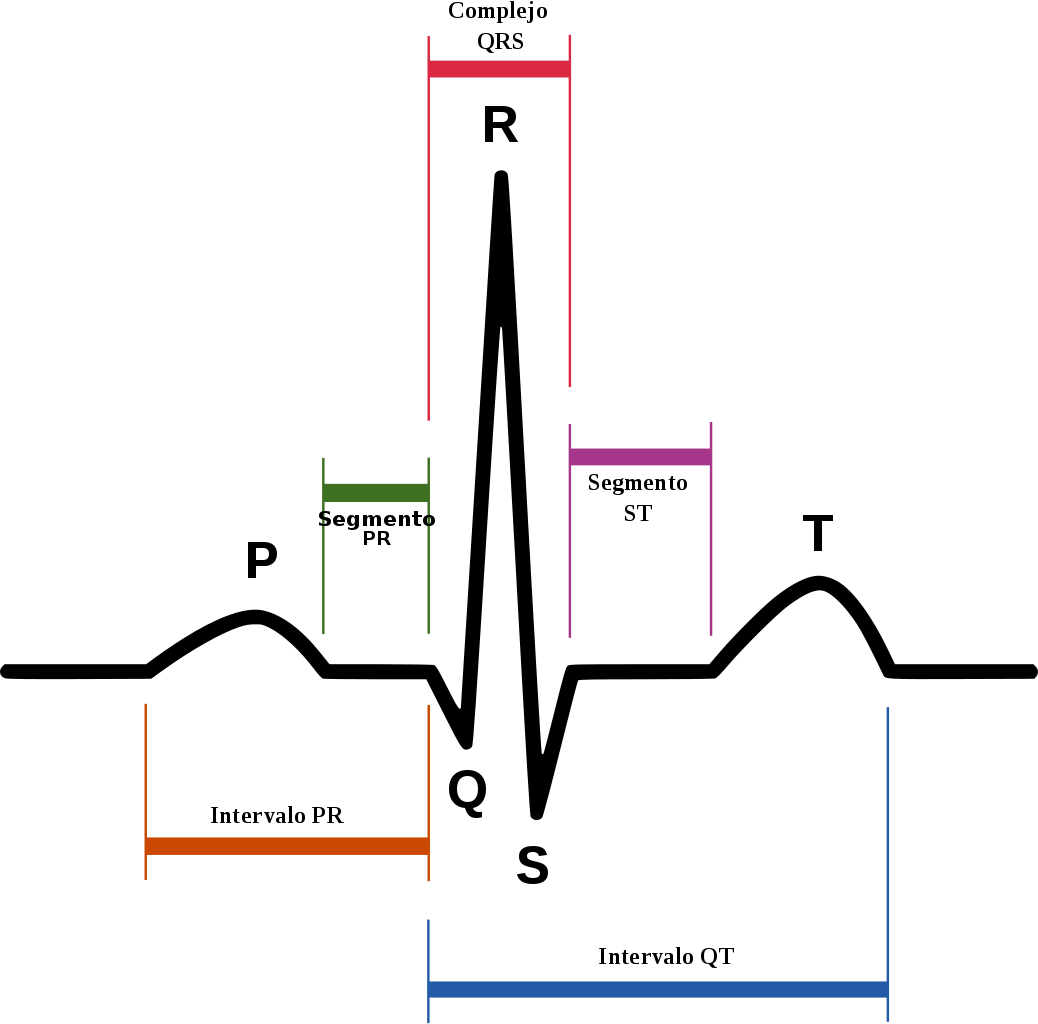
\includegraphics[width=0.5\linewidth]{Sem_1/figuras/1038px-SinusRhythmLabels-es.svg}
    	\caption{ECG con ritmo sinusal normal y las partes, segmentos e intervalos de este, debidamente identificadas}
    	\label{fig:ECGSinusal}
    \end{figure}
    \\
    
    Como se observa en la figura \ref{fig:ECGSinusal} el ECG consta de varias ondas representativas de cada etapa de un latido cardíaco, estas son: \\	
	\begin{itemize}
		\item \textbf{Onda P}: registra la despolarización auricular.
		\item \textbf{Complejo QRS}: Es la despolarización ventricular.
		\item \textbf{Onda T}: representa la repolarización ventricular.
	\end{itemize}
	
	Hoy en día el electrocardiograma es un estándar y uno de los primeros exámenes que se le hacen a los pacientes enfermos al ingresar a un centro clínico, este es registrado en un formato especialmente adaptado (tiras de papel milimetrado), estos no suelen durar más de 30 segundos. También puede ser registrada y visualizada de manera continua en un monitor similar a una pantalla de televisión, que suele ser una opción utilizada fundamentalmente en unidades de transporte sanitario medicalizadas y en unidades coronarias o de cuidados intensivos. \\
	\\
	Para intentar comprender los principios básicos que explican las oscilaciones en las líneas del ECG conviene conocer, si bien de forma somera, los fundamentos por los cuales se produce el movimiento del corazón, generado a través de microcorrientes eléctricas. De ellos es responsable el sistema de conducción eléctrica del corazón.
	
	\subsection{El sistema de conducción}
	Los impulsos eléctricos en el corazón se conducen mediante un tejido especializado al que se le denomina como sistema de conducción, este se puede describir como una intrincada red de cables a través de los cuales, y de un manera organizada, se realiza la transmisión de las microcorrientes eléctricas que generas el movimiento del corazón. La representación gráfica de estos impulsos (de estas microcorrientes) es el ECG. \\
	En el corazón normal, la frecuencia cardíaca debe ajustarse a las necesidades concretas que en un determinado momento se precisen (no tenemos las mismas pulsaciones durante el sueño que después de subir cuatro pisos). Por otro lado, las diferentes cámaras (aurículas y ventrículos) deben tener un movimiento sincronizado para que el latido cardíaco resulte eficaz. La sincronía del latido cardíaco, así como la fuerza en la contracción del corazón, se encuentran reguladas, entre otros factores, por el sistema de conducción, que consta de los siguientes elementos: 
	\begin{itemize}
		\item Nodo sinoauricular (nodo SA).
		\item Nodo auriculoventricular (nodo AV).
		\item Sistema de His-Purkinje.
	\end{itemize}
	
	\subsubsection*{El nodo sinoauricular (nodo SA)} 
	Está situado en el surco terminal entre la unión lateral de la vena cava superior con la aurícula derecha. Tiene una forma de huso con una cola larga dirigida hacia abajo por el surco terminal y en dirección del orificio de la vena cava inferior, está irrigado por la arteria nodal, rama de la arteria coronaria derecha en el $55\%$ de las veces y el resto por una rama de la arteria circunfleja. La conducción del impulso generado en el nodo, y que llega al nódulo auriculoventricular, se produce a través del músculo miocárdico auricular que por su disposición geométrica favorece la conducción preferencial \cite{fbbva}. 
	\subsubsection*{El nodo auriculoventricular (nodo AV)}
	Está localizado en el componente auricular del tabique auriculoventricular muscular, se halla subendocárdico y a la altura del vértice del triángulo delineado por el tendón de Todaro y en la inserción de la valva septal de la válvula tricúspide, estructuras que se unen en el cuerpo fibroso central. Aquí el nodo se continúa como el fascículo auriculoventricular que penetra el cuerpo fibroso y alcanza la cresta del tabique interventricular muscular debajo del septo membranoso y se bifurca en una rama derecha e izquierda. La rama derecha con un fascículo redondeado que hacia adelante se continúa hasta la región apical, penetra en la trabécula septomarginal y alcanza la pared ventricular y al musculo papilar anterior. Sus fibras forman el plexo subendocárdico de Purkinje en los músculos papilares y la pared del ventrículo derecho. Su tamaño es la mitad que el del nodo SA. Durante el paso por el nodo AV, la onda de activación eléctrica sufre una pausa de aproximadamente una décima de segundo, permitiendo así que las aurículas se contraigan y vacíen su contenido de sangre en los ventrículos antes de producirse la propia contracción ventricular. El nodo AV ejercería de esta forma un \textit{efecto embudo} en la canalización de los impulsos eléctricos en su viaje desde las aurículas a los ventrículos \cite{fbbva}.
	\subsubsection{Sistema de His-Purkinje}
	Después de atravesar el nodo AV, el impulso cardíaco se propaga por el haz de His y sus ramas ---una serie de fibras especializadas en la conducción eléctrica que discurren de arriba hacia abajo a lo largo del tabique interventricular; dicho haz de His de divide, después de un tronco común, en dos ramas, izquierda y derecha---. Cuando se emplea la expresión \textit{bloqueo de rama izquierda o bloqueo de rama derecha} se hace referencia a la interrupción de la transmisión de los impulsos eléctricos en el corazón en este nivel. Después de atravesar el haz de His, el impulso eléctrico se distribuye por toda la masa ventricular gracias a una red de microfibrillas denominadas fibras de Purkinje; se produce entonces la contracción (y consiguiente expulsión de la sangre) de ambos ventrículos \cite{fbbva}.
	\begin{figure}[h]
		\centering
		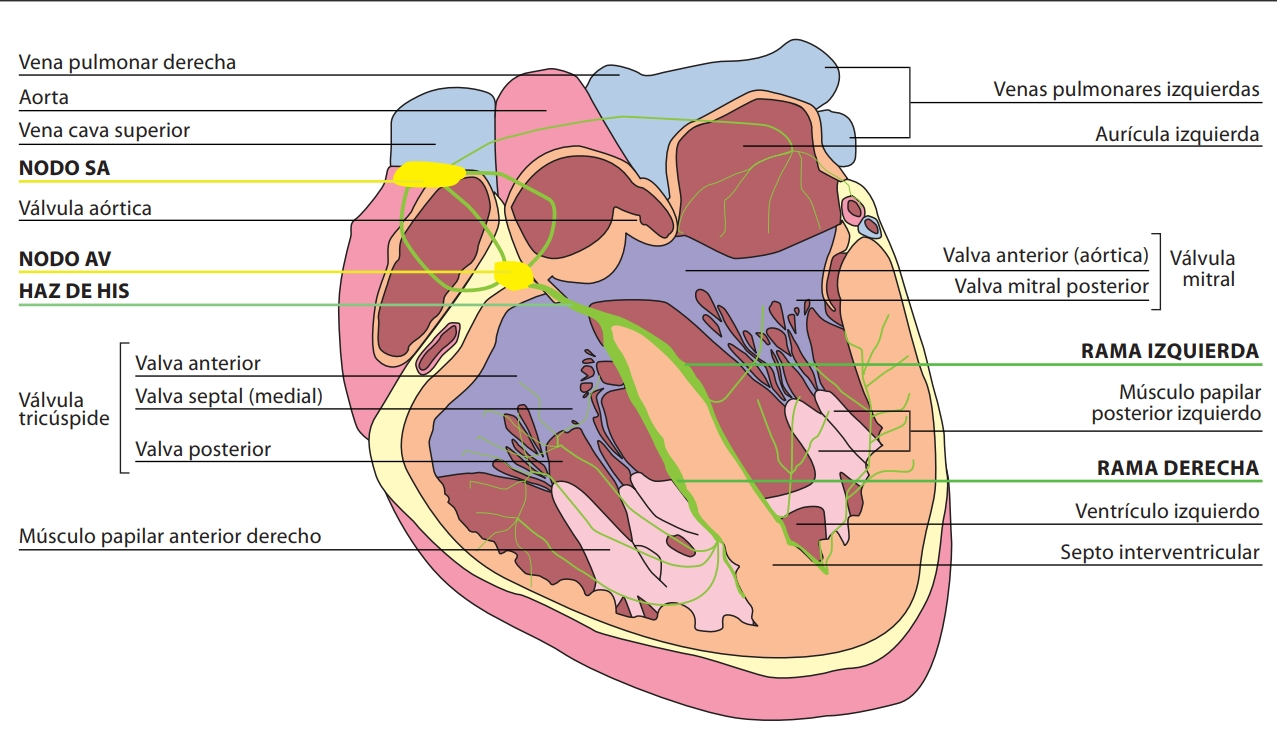
\includegraphics[width=0.95\linewidth]{Sem_1/figuras/Sistema_de_conduccion_corazon.jpeg}
		\caption{Sistema de conducción del corazón \cite{fbbva}.}
		\label{fig:sis_cond_heart}
	\end{figure}
	\subsubsection*{Actividad eléctrica de la célula miocárdica}
	La célula cardíaca posee, como las demás, una membrana celular que tiene en reposo una diferencia de voltaje entre sus dos lados. En condiciones normales y reposo, esta diferencia es de 90 milivoltios (mV). Debido a las propiedades intrínsecas de la célula, si esta es excitada, se desencadena una serie de cambios en la membrana que generan una corriente eléctrica que recorre la membrana celular y transmite el impulso eléctrico por los discos intercalares, que son membranas de baja resistencia eléctrica, entre las células, generando el potencial de acción. En el corazón normal este impulso se inicia en el nodo sinusal, debido a que tiene la descarga espontánea intermitente de frecuencia más alta en el corazón, gracias a las propiedades peculiares de la primera fase del potencial de acción en ese tejido. La disminución del potencial negativo de reposo despolariza la célula y luego se repolariza por la acción de mecanismos energéticos transmembrana que restablecen las concentraciones relativas de los iones, consumiendo energía (figura \ref{fig:fonocardio}) \cite{textCardi}.
	\begin{figure}[h]
		\centering
		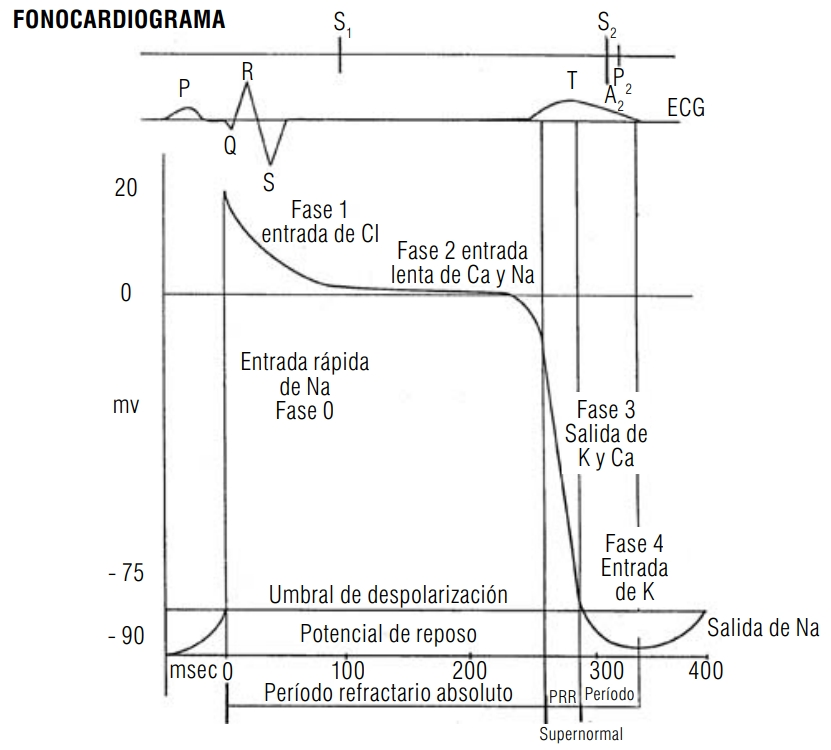
\includegraphics[width=0.8\linewidth]{Sem_1/figuras/fonocardiograma.jpeg}
		\caption{Potencial de acción-relaciones de componentes \cite{textCardi}.}
		\label{fig:fonocardio}
	\end{figure}
	Este potencial de acción conducido en forma adecuada es el estímulo para obtener una contracción cardíaca sincronizada. En reposo, el sodio está en el espacio extracelular en mayor concentración, al igual que el calcio, mientras que el potasio predomina en el espacio intracelular. Esto significa que la membrana tendrá una carga positiva por fuera y negativa por dentro. Al iniciarse la despolarización, ocurren cambios de la permeabilidad al sodio, lo cual permite su entrada al espacio intracelular, se invierte la carga interna, que se vuelve positiva ($+20$ mV) y la forma la fase 0 del potencial de acción. La pendiente de su ascenso regula la velocidad de conducción del tejido. Posteriormente, el cloro entra en persecución del sodio y disminuye levemente la positividad interior (fase 1). Luego baja drásticamente la permeabilidad al sodio y calcio y estos iones comienzan a disminuir su velocidad de entrada, la cual se hace básicamente a través de los canales lentos, que son voltaje dependientes y de tipo receptor de membrana que consume energía, y que inscriben una fase en meseta en el potencial de acción (Fase 2). Los canales lentos de calcio son altamente selectivos para este ion, aunque permiten la entrada también de sodio. Este mecanismo en la membrana del retículo sarcoplásmico asegura, además, que la concentración intracelular de calcio sea suficiente para los procesos contráctiles. Inmediatamente sale potasio de la célula para lograr el equilibrio de cargas eléctricas, al parecer por un súbito aumento de la permeabilidad de la membrana para este ion, disminuye la positividad y logra un potencial negativo intenso intracelular, saliendo calcio al retículo sarcoplásmico nuevamente (Fase 3). Esto repolariza la célula. Pero luego entran en acción las bombas de sodio y calcio, dependientes de ATP, que sacan Na y CA y lo intercambian por potasio, lo cual incrementa levemente el potencial intracelular (Fase 4).
	
	La velocidad de ascenso de la fase 4 es lo que regula la excitabilidad y es más pronunciado en los tejidos de excitación automática. El calcio que entra en la fase 2 es aclarado de la célula por varios mecanismos como son: las bombas de calcio dependientes de ATP, el fosfolamban, y la captación de calcio hacia el interior de la mitocondria, en un proceso que también es dependiente de energía. El potencial de acción tiene una duración variable (entre 200 y 400 ms) y durante ese período, la célula se hace total o parcialmente refractaria a una excitación adicional, al parecer por la presencia de sodio dentro de la célula. El periodo refractario absoluto ocupa las fases 0, 1, 2 y 3, es decir, mientras el sodio es aún intracelular. Una vez que el sodio comienza a salir de la célula, está parcialmente disponible para volver a entrar rápidamente, por lo que la fase 4 y la parte final de la fase 3 son el período refractario relativo. El potencial más negativo que se alcanza durante la fase 4 se atenúa en presencia de Ácidosis, hipocalemia isquemia y fibrosis y se aumenta con los medicamentos antiarrítmicos en su mayoría. Existen diferencias en la configuración del potencial de acción según el tejido analizado dentro del corazón: en las células automáticas, las fases 1 y 2 son cortas y la fase 4 es plana y en las células de conducción, la fase 0 es rápida, y la fase 2 es de mayor duración. Las fases 0 y 1 corresponden a la onda P y el complejo QRS. La fase 2 corresponde al segmento ST y la fase 3 a la onda T. La fase 4 corresponde a la diástole eléctrica. La deflexión descendente de la onda T corresponde al período refractario relativo, que tiene 2 subfases: la vulnerable que es durante la cual un estímulo de suficiente intensidad es capaz de desencadenar arritmias severas, y la subfase súper-normal, que corresponde a una hiperpolarización "muy refractaria", pues no hay potasio intracelular en cantidad abundante. La velocidad a la cual se transmite el impulso varía de acuerdo con la pendiente de la fase 0, con la altura del potencial de acción, con la duración de las fases 2 y 4. Dicha velocidad en el nodo sinusal es de $5 cm/s$, en las aurículas es de $80-100 cm/s$, en el nodo AV es de $5 cm/s$, en el haz de His es de $100 cm/s$, en las fibras de Purkinje es de $400 cm/s$ y en el músculo de $90 cm/s$
	
	Las células miocárdicas tienen varias propiedades únicas, entre ellas está la Automaticidad que no es más que la capacidad de descarga espontánea a una frecuencia fija, dependiente de la pendiente de la fase 4; La Excitabilidad es esa capacidad de respuesta al estímulo; y por último, la Conductividad que es esa capacidad de transmitir el impulso de una célula a otra.
	
\subsection{Interpretación de un electrocardiograma}

El ECG presenta como línea guía la denominada \textit{línea isoeléctrica o línea basal}, que puede identificarse fácilmente como la línea horizontal existente entre cada latido. Los latidos cardíacos quedan representados en el ECG \textit{normal} por las diferentes oscilaciones de la línea basal en forma de ángulos, segmentos, ondas e intervalos, constituyendo una imagen característica que se repite con una frecuencia regular a lo largo de la tira de papel del ECG. Como se ha comentado, entre latido y latido va discurriendo la línea base. \\
El recorrido en sentido horizontal hace referencia al \textit{tiempo} transcurrido, y la distancia en sentido vertical (amplitud) al \textit{voltaje} que se está produciendo. El papel por el que discurre el registro de la línea se encuentra milimetrado. Cada cuadrado pequeño del papel mide $1 mm$ y al observarlo con detenimiento puede comprobarse que cinco cuadrados pequeños forman un cuadrado grande, remarcado por un grosor mayor en la tira de papel de ECG. Para conocer cómo transcurren los tiempos durante la actividad del corazón, basta con recordar que cinco cuadrados grandes en sentido horizontal equivalen exactamente a un segundo. \\
En un ECG \textit{normal}, cada complejo consta de un a serie de deflexiones (ondas del ECG) que alternan con la línea basal. Realizando la lectura de izquierda a derecha, se distinguen la onda P, sel segmento P-R, el complejo QRS, el segmento ST y finalmente la onda T, véase la figura \ref{fig:ECGSinusal}.
\subsubsection{Onda P}

Es la primera deflexión hacia arriba que aparece en el ECG. Su forma recuerda a una mezcla entre una U y una V invertidas. Suele durar entre $80-100 ms$ y esta representa el momento en que las aurículas se están contrayendo y enviando sangre hacia los ventrículos. 

\subsubsection{Segmento P-R}

Es el tramo de la línea basal (línea isoeléctrica) que se encuentra entre el final de la onda P y la siguiente deflexión ---que puede ser hacia arriba (positiva) o hacia abajo (negativa)--- del ECG. Durante este período, las aurículas terminan de vaciarse y se produce una relativa desaceleración en la transmisión de la corriente eléctrica a través del corazón, justo antes del inicio de la contracción de los ventrículos. 

\subsubsection{Complejos QRS}

Corresponde con el momento en que los ventrículos se contraen y expulsan su contenido sanguíneo. Como su nombre indica, consta de las ondas Q, R y S. La onda Q no siempre está presente. Se identifica por ser la primera deflexión negativa presente después del segmento P-R. Toda la deflexión positiva que aparezca después del segmento P-R corresponde ya a la onda R propiamente dicha y, como se ha comentado anteriormente, el hecho de que no vaya precedida por una onda Q no es en absoluto patológico. De hecho, y siempre en relación con una ECG normal, las ondas Q deben ser de pequeño tamaño ---no mayores que un cuadrado pequeño en el papel milimetrado, tanto en longitud (duración) como en profundidad (voltaje)--- y encontrarse presentes sólo en ciertas derivaciones. La onda R es muy variable en altura, ya que puede llegar a medir desde $2 mm$ hasta $8-10 mm$ en el caso de personas jóvenes deportistas. La onda S se observa como continuación directa de la onda R y comienza a partir del punto en que esta última, en su fase decreciente, se hace negativa.\\
En conjunto, el complejo formado por las ondas Q, R y S no debe exceder en duración más de dos cuadrados pequeños. 

\subsubsection{Segmento ST}

En el trazado de la línea basal que se encuentra entre el final de la onda S y el comienzo de la onda T. Su elevación o descenso en relación con la línea basal puede significar insuficiencia en el riego del corazón, especialmente si dichas oscilaciones coinciden con sintomatología característica que pueda expresar afectación en el aporte de oxígeno al corazón. En este sentido, su valor como herramienta diagnóstica resulta insustituible.

\subsubsection{Onda T}

Se inscribe a continuación del segmento ST. Consiste en una deflexión normalmente positiva que asemeja el relieve de una montaña más o menos simétrica. Su duración suele estar entre $0,1-0,25 s$ y no debe exceder los $0,3 s$. La onda T representa el momento en que el corazón se encuentra en un período de relajación, una vez que ha expulsado la sangre que se hallaba en los ventrículos.

\subsection{Realización de un electrocardiograma}

Realizar un ECG es un procedimiento sencillo. Se necesitan un electrocardiógrafo, parches de ECG que actúan como sensores sobre la piel, comportándose como si fueran electrodos, y un sistema de cables que transmiten las microcorrientes recogidas por los parches al electrocardiógrafo, el cual se encargará de amplificarlas. El paciente se coloca boca arriba sobre una camilla. La postura ideal es completamente horizontal; en caso de no tolerar bien esta posición, la camilla podría elevarse unos treinta grados. \\
Un enfermero, un técnico o un médico le colocarán un total de 10 parches (electrodos). Se coloca uno en cada extremidad, formando así las seis derivaciones llamadas \textit{de los miembros}. Los restantes seis parches se colocan en seis puntos específicos del pecho en la denominada \textit{región precordial}, y hacen referencia a las seis derivaciones precordiales. Una derivación electrocardiográfica está constituida por la unión de dos electrodos. De esta forma, es posible conseguir un total de 12 derivaciones. Cada una permite obtener una visión electrocardiográfica diferente, representando 12 \textit{ventanas} o puntos de observación distintos. Así, una anomalía que afecta a una parte concreta del corazón puede no ser advertida desde una derivación (ventana) y sí desde otra. Esta característica confiere valor al ECG para localizar la zona del corazón que puede encontrarse dañada. Cada derivación presenta un patrón del ECG característico con el que el médico está familiarizado, pero los principios expuestos en la descripción del ECG son aplicables a todas las derivaciones. \\
Una vez que el paciente se encuentra tumbado y con los 10 cables que conectan el ECG con su parche (electrodo) correspondiente, se puede comenzar el registro del ECG, cuya duración aproximada es de 10 segundos. El registro obtenido ---gracias a la impresora que lleva incorporado el propio ECG--- constituye el ECG del paciente. 

Es importante tener en cuenta que desde el momento en que el operador indica que va a comenzar el registro, el paciente debe moverse lo menos posible, ya que incluso el temblor muscular fino (por ejemplo, por frío o intranquilidad) puede interferir con la señal del registro, y en el caso de resultar excesivamente distorsionada será preciso repetir el ECG. Asimismo, el contacto entre los parches y la piel del enfermo debe ser lo más estrecho posible y, en este sentido, al realizar un ECG hay que evitar la utilización previa de cremas o lociones que interfieran en dicho contacto. Es frecuente que el operador tenga que emplear una gasa suavemente impregnada en alcohol, ya que la propia grasa de la piel puede interferir con la nitidez del registro, y aplicarla sobre los puntos donde serán situados los parches.

Éstos llevan un gel autoadhesivo cuya composición favorece la transmisión de las pequeñas corrientes eléctricas desde la piel al electrocardiógrafo. Este gel conductor tiene una caducidad relativamente temprana y ocasionalmente puede ocurrir que la señal eléctrica no pueda ser recogida por el electrocardiógrafo debido a anomalías o defectos del parche. En este caso, en el papel del ECG no aparecerá ningún tipo de señal, ninguna línea. Naturalmente, la situación queda subsanada en cuanto se desprendan los parches defectuosos y se repita el ECG utilizando los adecuados. 

Hoy en día, un ECG puede ser realizado en cualquier sitio debido tanto a la reducción en el tamaño de los equipos como, sobre todo, a la posibilidad de disponer el electrocardiógrafos portátiles. De esta forma, el ECG llega al domicilio de pacientes que no se pueden desplazar o al lugar donde se ha producido un accidente y, naturalmente, se puede disponer de monitorización con ECG continua durante el transporte sanitario. Pese a todo, lo más frecuente es que el ECG se realice dentro del medio hospitalario o bien a nivel ambulatorio en centros de salud o consultorios médicos.

Existen otras formas de realizar un ECG aparte de la convencional en reposo. Fundamentalmente son dos: el ECG de esfuerzo que consiste en caminar en una cinta sin fin o pedalear en una bicicleta especialmente adaptada, mientas un médico valore el ECG realizado durante el ejercicio, y el Holter-ECG, en el que se registra el ECG del paciente mediante un sistema de grabación especialmente diseñado, durante un tiempo aproximado de 24 horas; posteriormente, es analizado por un \textit{software} específico y este, se utiliza principalmente para el estudio de arritmias \cite{textCardi}. 

El ECG es una prueba diagnóstica asequible, segura y sencilla de realizar, que proporciona una gran cantidad de información con relación al estado del corazón. Fundamentalmente, se utiliza para detectar trastornos del ritmo cardíaco (arritmias) y en el diagnóstico de trastornos del flujo coronario, como lo son las cardiopatías coronarias. Asimismo, el ECG es el método de elección en el diagnóstico de los bloqueos cardíacos, en los cuales la transmisión del impulso ha quedado parcial o completamente interrumpida en algún de su recorrido a través del sistema de conducción. El ECG también se utiliza, aunque en menor medida, en el diagnóstico del aumento de tamaño de las cavidades del corazón. Este hecho se observa muy frecuentemente en la hipertensión arterial, en la cual el corazón tiene que bombear contra una resistencia que se encuentra aumentada. También, algunos trastornos de los electrolitos sanguíneos, especialmente el calcio y el potasio, tienen también su reflejo en el ECG, que naturalmente su nivel exacto se obtendrá a través de un análisis de sangre, pero el ECG puede resultar orientativo en cuanto al grado de gravedad de la alteración. Finalmente, el ECG también resulta útil en el seguimiento de las enfermedades cardíacas al establecerse una comparación con los electros previos del paciente. Así, ayuda al médico a valorar el desarrollo evolutivo de una determinada patología y, en ocasiones, es de gran utilidad a la hora de establecer un tratamiento concreto o de modificar la dosis de algún medicamento que el paciente pueda estar tomando. 

Para efectuar un ECG no se precisa ninguna preparación en concreto, además que no existen riesgos en la realización de un ECG, ya que es una prueba segura y exenta de ellos. La actividad eléctrica reflejada en el papel es generada por el propio organismo, de ahí que el paciente no sienta nada durante el registro. 

\section{Conceptos específicos}

\subsection{Aprendizaje Automático.}
	El aprendizaje automático se ha vuelto uno de los más importantes temas hoy en día, constantemente se busca la manera de sacar el mayor provecho de los datos que se tengan recopilados con el fin de desarrollar estrategias que ayuden a tener un nivel superior de entendimiento de estos. Con los modelos de aprendizaje automático apropiados, se tiene la habilidad de hacer predicciones precisas en el mundo real y a medida que nueva data es constantemente agregada, se asegura que los modelos continúen rindiendo eficientemente y siendo capaces de adaptarse a los problemas del mundo real. 

	El aprendizaje automático es una de las ramas de la Inteligencia Artificial (IA) que le permite a un sistema aprender de los datos que se le dan en lugar de programarle explícitamente la tarea que debe desempeñar. 
	
	El aprendizaje automático usa una variedad de algoritmos que interactivamente aprenden de los datos, para mejorar, describir datos e incluso, predecir resultados. Como estos algoritmos constantemente ingieren datos de entrenamiento, es entonces posible producir modelos más precisos basados con esta data. El aprendizaje automático engloba tantos algoritmos que es necesario agruparlos por categorías o paradigmas de aprendizaje, estos se dividen en función de la salida de los mismos.

\subsection{Análisis de Componentes Principales (PCA).} \label{subsec:PCA}
	Los grandes conjuntos de datos están cada vez más extendidos en muchas disciplinas. Para interpretarlos, se necesitan métodos que reduzcan drásticamente su dimensionalidad de forma interpretable, de modo que se conserve la mayor parte de la información contenida en los datos. Se han desarrollado muchas técnicas con este fin, pero el análisis de componentes principales (PCA) es una de las más antiguas y utilizadas. Su idea es sencilla: reducir la dimensionalidad de un conjunto de datos conservando la mayor cantidad posible de «variabilidad», es decir, de información estadística.
	
	Esto significa que «preservar tanta variabilidad como sea posible» se traduce en encontrar nuevas variables que sean funciones lineales de las del conjunto de datos original, que maximicen sucesivamente la varianza y que no estén correlacionadas entre sí. PCA usa álgebra lineal para transformar datos a unas variables llamadas componentes principales (PC). Estas se encuentras calculando los autovectores (direcciones) y autovalores (importancia) de una matriz de covarianza. PCA selecciona los componentes principales con los autovalores más altos y proyecta los datos sobre ellos, para simplificar el conjunto de datos. Para esto se debe: \\
	\begin{enumerate}
		\item \textbf{Estandarizar los datos.} \\
		Las diferentes caracteristicas que están presentes en el conjunto de datos pueden tener diferentes unidades y escalas. Para comparar estas equitativamente, primero se debe estandarizar los datos haciendo que cada característica tenga: 
		\begin{itemize}
			\item Una media de $0$.
			\item Una desviación estándar de $1$.
		\end{itemize}
		\begin{equation}
			\label{eq:standard}
			Z = \frac{\textit{X}-\mu}{\sigma}
		\end{equation}
		donde:
		\begin{itemize}
			\item $\mu$ es la media de las características independientes $\mu = \{\mu_1, \mu_2,\dotsb,\mu_m\}$
			\item $\sigma$ es la desviación estándar de las características independientes $\sigma = \{\sigma_1, \sigma_2,\dotsb,\sigma_m\}$
		\end{itemize}
		\item \textbf{Calcular la matriz de covarianza.}\\
		Es necesario calcular la matriz de covarianza para ver como las características se relacionan entre sí, si estas aumentan o disminuyen juntas. La matriz de covarianza entre dos características $x_1$ y $x_2$ es:
		\begin{equation}
			\label{eq:covarianza}
			\operatorname{cov}(x 1, x 2)=\frac{\sum_{i=1}^n\left(x 1_i-\bar{x} 1\right)\left(x 2_i-\bar{x} 2\right)}{n-1}
		\end{equation}
		donde: 
		\begin{itemize}
			\item $\bar{x}_1$ y $\bar{x}_2$ son los valores medios de las características $x_1$ y $x_2$.
			\item $n$ es el numero total de datos.
		\end{itemize}
		El valor de la covarianza puede ser positivo, negativo o cero.
		\item \textbf{Encontrar las componentes principales.}
		PCA identifica los \textit{nuevos ejes} donde la varianza de los datos es mayor:
		\begin{itemize}
			\item \textbf{1er Componente Principal (PC1):} La dirección donde está la mayor dispersión de los datos.
			\item \textbf{2da Componente Principal (PC2):} La siguiente mejor dirección, \textit{perpendicular a PC1} y así sucesivamente.
		\end{itemize}
		Estas direcciones vienen de los autovectores de la matriz de covarianza y su importancia es medida por los autovalores. Para una matriz $A$, un autovector $X$ (un vector no nulo) y su correspondiente autovalor $\lambda$ satisface:
		\begin{equation}
			\label{eq:autovalores}
			AX = \lambda X
		\end{equation}
		Esto significa:
		\begin{itemize}
			\item Cuando $A$ actuá sobre $X$ sólo estira o encoge $X$ por el escalar $\lambda$.
			\item La dirección de $X$ no cambia, por lo que los autovectores definen \guillemetleft direcciones estables\guillemetright \ de $A$.
		\end{itemize}
		\item \textbf{¿Cuantas dimensiones se deberían calcular?}
		Una de las preguntas claves en este punto es cuantas PCs conservar. Entre todas las maneras de responder esta interrogante, uno de los métodos más populares es la \emph{suma de la varianza acumulada}, este método ha sido usado en muchas librerías y paquetes de algunos lenguajes como Python y MATLAB. \\
		En PCA, cada componente principal representa una dirección de máxima varianza de los datos a esta se le conoce como la \emph{varianza explicada}, esta mide cuanta información (o dispersión) de los datos originales captura dicha PC. La \emph{varianza explicada acumulada} es la suma de las varianzas explicadas por los componentes principales seleccionados hasta cierto punto, expresada como un porcentaje del total. Este valor permite determinar qué proporción de la información total del conjunto de datos que se conserva al incluir un número específico de componentes. Para esto basta con calcular el acumulativo de las varianzas de las componentes principales para luego definir un umbral deseado que será el porcentaje de retención de información preferido según los requerimientos del problema, por ultimo basta con identificar el menor numero de componentes necesarios para superar el umbral deseado. En la figura \ref{fig:varianza_acumulada} se observa un ejemplo grafico de lo anteriormente dicho.
		\item \textbf{Selecciona las mejores direcciones y transforma los datos.}
		Después de calcular los autovalores y autovectores, PCA clasifica estos por la cantidad de información que ellos capturan. Entonces: 
		\begin{itemize}
			\item Selecciona los k componentes principales que capturan la mayor parte de la varianza, como el 95\%.
			\item Transforma el conjunto de datos original proyectándolo sobre los mejores componentes principales. 
		\end{itemize}
		Esto significa que se reduce el numero de características (dimensiones) mientras se mantienen los patrones importantes que están implícitos de los datos.
	\end{enumerate}
	
	Hasta que no se generalizó el uso de ordenadores electrónicos, que fue posible utilizarlo con conjuntos de datos que no fueran trivialmente pequeños. Desde entonces, su uso se ha multiplicado y se han desarrollado numerosas variantes en muchas disciplinas diferentes.
	
	\begin{figure}[h]
		\centering
		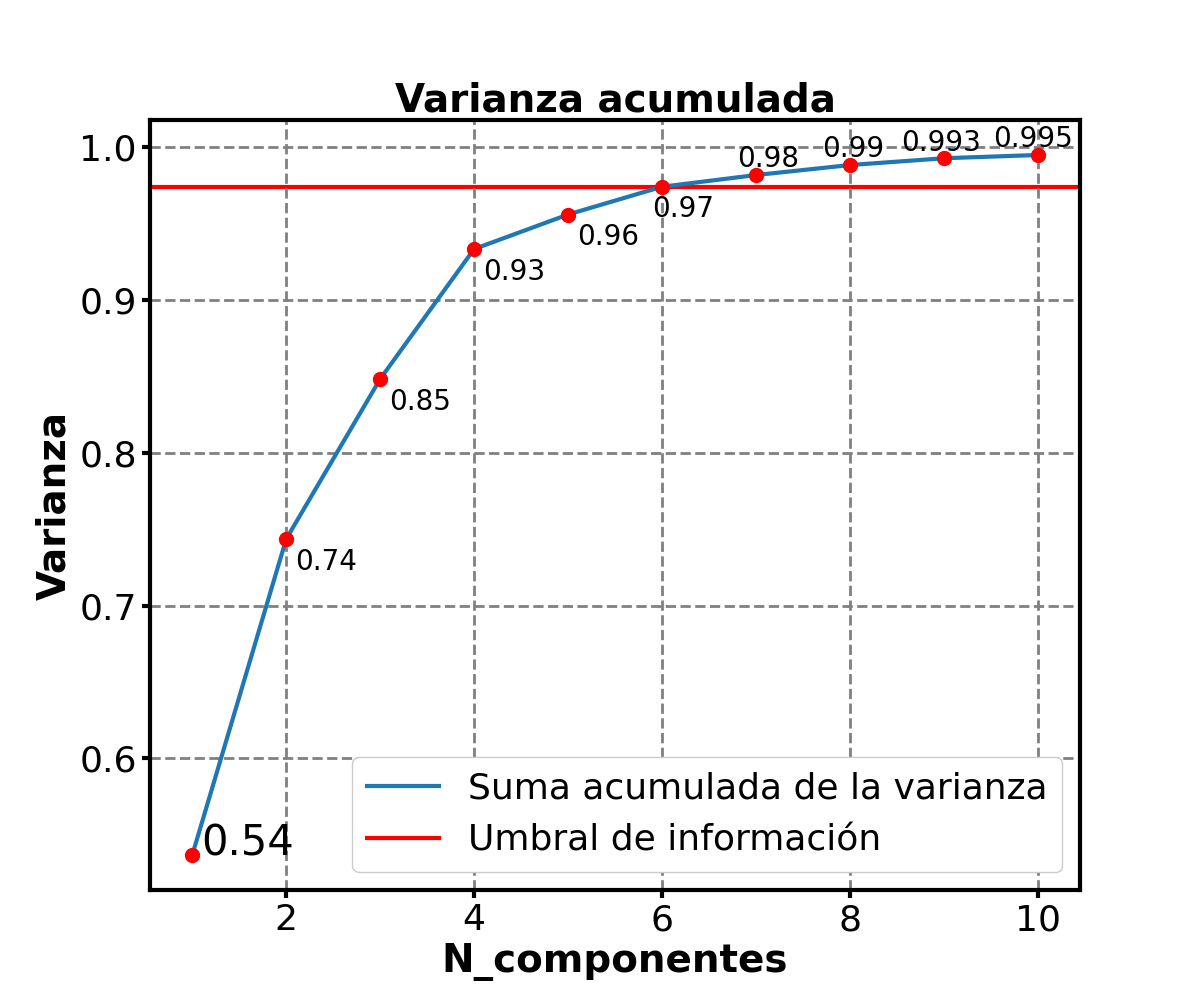
\includegraphics[width=0.8\linewidth]{Sem_1/figuras/suma_acumulada_varianza.png}
		\caption{Varianza acumulada frente al número de componentes principales en un conjunto de datos de ejemplo.}
		\label{fig:varianza_acumulada}
	\end{figure}
	
%	La definición formal de PCA, en un contexto estándar, junto con una derivación que muestra que puede obtenerse como la solución a un problema de auto-valores y auto-vectores o, alternativamente, a partir de la descomposición del valor singular (SVD) de la matriz (centrada) de datos. El PCA puede basarse en la matriz de covarianzas o en la matriz de correlaciones. Se discutirá la elección entre estos análisis. En ambos casos, las nuevas variables (las PC) dependen del conjunto de datos, en lugar de ser funciones de base predefinidas, por lo que son adaptativas en sentido amplio. Los principales usos del PCA son descriptivos y no inferenciales.\cite{Joliiffe16}\\

\subsection{Incrustación de vecinos estocásticos distribuidos en t (t-SNE).}
	\label{subsec:tsne}
	 La incrustación de vecinos estocásticos comienza convirtiendo las distancias Euclidianas altas dimensionales entre los puntos de datos en probabilidades condicionales que representan similaridades. Según van der Maaten y Hinton: "La similaridad entre el punto $x_i$ $x_j$ es proporcional a la probabilidad condicional $p_{i\mid j}$ de que $x_i$ escoja a $x_j$ como su vecino si los vecinos se eligieran en proporción a su densidad de probabilidad bajo una gaussiana centrada en $x_i$". Para puntos de datos cercanos, $p_{i\mid j}$ es relativamente alta, mientras que para puntos de datos muy separados, $p_{i\mid j}$ será casi infinitesimal (para valores razonables de la varianza en la gaussiana, $\sigma_i$). Matemáticamente, la probabilidad condicional $p_{i\mid j}$ es dada por: 
	 \begin{equation}
	 	\label{eq:prob_cond}
	 	p_{j \mid i}=\frac{\exp \left(-\left\|x_i-x_j\right\|^2 / 2 \sigma_i^2\right)}{\sum_{k \neq i} \exp \left(-\left\|x_i-x_k\right\|^2 / 2 \sigma_i^2\right)},
	 \end{equation}
	donde $\sigma_i$ es la varianza de la Gaussiana que está centrada en el punto $x_i$. Debido a que estamos interesados en modelar las similaridades entre pares, se establece $p_{i\mid j} = 0$. Observe que el denominador anterior garantiza $\sum_j p_{j \mid i}=1$ para todas las $i$. Para las contrapartes de baja dimensionalidad $y_i$ y $y_j$ de los puntos altos dimensionales $x_i$ y $x_j$, es posible calcular una probabilidad condicional similar, la cual se denotará por $q_{j \mid i}$. De ahí que, se modela la similaridad de un punto cartográfico $y_j$ con el punto cartográfico $y_i$ por:
	\begin{equation}
		\label{eq:prob_cond_q}
		q_{j \mid i}=\frac{\exp \left(-\left\|y_i-y_j\right\|^2\right)}{\sum_{k \neq i} \exp \left(-\left\|y_i-y_k\right\|^2\right)}
	\end{equation}
	
	Al igual que en el caso anterior, como sólo se está interesado en el modelado de las similaridades en cada par de puntos, se establece $q_{i \mid i}=0$.
	Las probabilidades condicionales $q_{i \mid i}$ y $p_{i \mid i}$ serán iguales siempre y cuando los puntos cartográficos $y_i$ y $y_j$ modelen correctamente la similaridad entre los puntos alto dimensiones $x_i$ y $x_j$.
	
	En este caso, se utiliza una distribución t de Student de colas gruesas para medir las similitudes entre puntos cartográficos de baja dimensión, con el fin de permitir que los objetos se modelen muy separados entre si. 
	Se busca una representación bajo dimensional de los datos que minimice la disparidad entre $q_{i \mid i}$ y $p_{i \mid i}$, para lograr esto, se usa como medida de fidelidad entre $q_{i \mid i}$ y $p_{i \mid i}$, la divergencia de Kullback-Leibler. Haciendo uso del método de gradiente descendiente t-SNE, minimiza la suma de las divergencias de Kullback-Leibler sobre todos los puntos, teniendo una función de costo dada por: 
	\begin{equation}
		\label{eq:func_costo}
		C = \sum_i KL(P_i\|Q_i)=\sum_i\sum_j p_{j\mid i}\log\frac{p_{j\mid i}}{q_{j\mid i}},
	\end{equation}
	en la cual $P_i$ representa la distribución de probabilidad condicional sobre todos los puntos de datos, dado el punto $x_i$, y $Q_i$ representa la distribución de probabilidad condicional sobre todos los puntos de datos, dado el punto $y_i$ y es el resultado de esta optimización, un mapa que refleja las similitudes entre las entradas de alta dimensión.
%	Aca estoy dudoso si también hablar sobre el perplexity y todo lo que viene despues de eso
%	Al final no lo puse
	
%\subsection{K-medios (k-means).}

%	Los problemas de agrupamiento aparecen en diferentes aplicaciones, como reconocimiento y clasificación de patrones, de acá surge en la búsqueda de algoritmos que permitan visualizar los datos en forma de grupos o \textit{clusters}\footnote{Cúmulo, grupo o racimo}. La noción de lo que constituye un buen clúster depende de su aplicación y de la aproximación con la que se llega a este. La mayoría de las formulaciones de los métodos de agrupamiento, están basadas en minimizar una función objetiva y quizás el algoritmo más usado y estudiado es \textit{k-means}. Dado un conjunto de puntos $\mathbf{x}=\{x_1,x_2,\dotsb,x_n\}$ en un espacio real \textit{d}-dimensional, $\mathbf{R}^d$, y un entero \textit{k} ($k \leq n$), el problema es entonces, determinar un conjunto de \textit{k} puntos en $\mathbf{R}^d$, llamados \textit{centroides} $S_k$, que minimicen la \textit{inercia} o la suma de cuadrados de cada grupo (WCSS, por sus siglas en inglés) desde para punto de los datos a su centroide más cercano, esto es: 
%	\begin{equation}
%		\label{eq:min_k_means}
%		\underset{\mathbf{S}}{\arg \min } \sum_{i=1}^k \sum_{\mathbf{x}_j \in S_i}\left\|\mathbf{x}_j-\boldsymbol{\mu}_i\right\|^2
%	\end{equation}
%	Se puede decir que la \textit{inercia} es una medida de que tal coherentes son los clusters internamente, esto lleva a que se sufran de algunos inconvenientes:
%	\begin{itemize}
%		\item La \textit{inercia} no es una métrica normalizada, por lo que en espacios muy alto dimensionales, las distancias Euclidianas tienden a volverse infladas (a esto se le llama "maldición de la dimensionalidad"). Es por esto que aplicar algoritmos de reducción de dimensionalidad como PCA previo a k-means, puede agilizar y aliviar el consumo computacional.
%		\item k-means responde ineficientemente a clusters alargados o grupos con formas irregulares, debido a que la \textit{inercia} presume que los clusters son convexos e isotrópicos.
%	\end{itemize}
%	El algoritmo estándar de k-means, fue propuesto inicialmente por Stuart Lloyd en 1957, quien lo propuso como una técnica para modulación por impulsos codificados, sin embargo este no fue publicado hasta 1982, es por esto que a este algoritmo también se le conoce como algoritmo de Lloyd, sobre todo en la comunidad informática. \\
%	
%	\textbf{Algoritmo k-means (basado en MacKay, 2003 \cite{mackay03}):}
%	\begin{enumerate}
%		\item \textbf{Inicialización:} 
%		Se eligen los $k$ centroides $\left\{\mathbf{m}^{(k)}\right\}$ aleatoriamente.
%		\item \textbf{Paso de asignación:}
%		Cada punto $\mathbf{x}^{(n)}$ se asigna al centroide más cercano. La asignación se denota como $\hat{k}^{(n)}$:
%		\begin{equation}
%			\label{eq:k_mean_asig}
%			\hat{k}^{(n)}=\underset{k}{\operatorname{argmin}}\left\{d\left(\mathbf{m}^{(k)}, \mathbf{x}^{(n)}\right)\right\}
%		\end{equation}
%		Una representación alternativa y equivalente de esta asignación de puntos a los conglomerados viene dada por las \textit{responsabilidades}, que son variables indicadoras $r_k^{(n)}$. En el paso de asignación, establecemos $r_k^{(n)}$ en uno si la media $k$ es la media más cercana al punto de datos $\mathbf{x^{(n)}}$; de lo contrario $r_k^{(n)}$ es cero.
%		\begin{equation}
%			\label{eq:cond_rk}
%			r_k^{(n)}=\left\{\begin{array}{lll}
%				1 & \text { si } & \hat{k}^{(n)}=k \\
%				0 & \text { si } & \hat{k}^{(n)} \neq k
%			\end{array}\right.
%		\end{equation}
%		\item \textbf{Paso de actualización:}
%		Los parámetros del modelo, las medias, se ajustan para que coincidan con las medias muestrales de los puntos de datos de los que son responsables.
%		\begin{equation}
%			\label{eq:media_muestral}
%			\mathbf{m}^{(k)}=\frac{\sum_n r_k^{(n)} \mathbf{x}^{(n)}}{R^{(k)}}
%		\end{equation}
%		donde $R^{(k)}$ es la \textit{responsabilidad} total de la media $k$.
%		\begin{equation}
%			\label{eq:rk}
%			R^{(k)}=\sum_n r_k^{(n)}
%		\end{equation}
%		\item \textbf{Se repiten los pasos de asignación y actualización} hasta que no hayan cambios en la asignación.
%	\end{enumerate}
	
\subsection{Redes Neuronales.} \label{subsec:NN}
	Una red neuronal artificial es un programa que intenta imitar la manera en que un cerebro humano es capaz de abordar ciertos problemas, esta usa capas interconectadas de unidades, llamadas perceptrones (también se les llama neuronas), siendo capaces de aprender e inferir reglas o relaciones basados en la data observada, dicha red adquiere los conocimientos mediante un proceso de entrenamiento y aprendizaje, donde este almacena \textit{conocimiento} utilizando intensidades de conexión interperceptrónica. 
	\subsection{Redes neuronales biológicas.}
	Es necesario entender el concepto de una red neuronal del tipo biológico para poder comprender que es lo imitan las redes neuronales artificiales, estas se definen como la unión de neuronas a otras generando así, un conjunto de conexiones sinápticas ordenadas. Las neuronas, no son más que células con características únicas que le permiten diferenciarse del resto de las células biológicas al poder comunicarse entre ellas. En la figura \ref{fig:neurona} se observan las partes de una neurona biológica. 
	\begin{figure}[h]
		\centering
		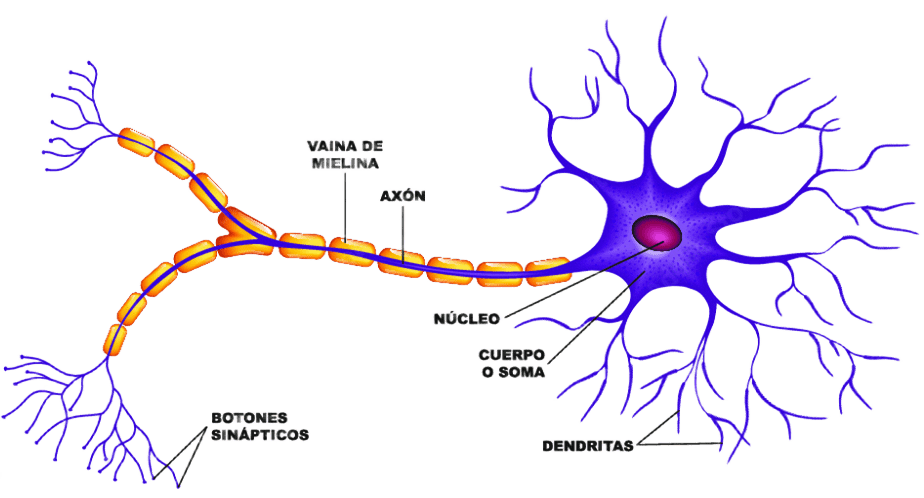
\includegraphics[width=0.6\linewidth]{Sem_1/figuras/neurona}
		\caption{Estructura de una neurona.\cite{imaNeu}.}
		\label{fig:neurona}
	\end{figure}
	
	Una neurona consta de tres partes:
	\begin{enumerate}
		\item El cuerpo de la neurona.
		\item Las dendritas, que reciben las entradas.
		\item El axón, que llave la salida de la neurona a las dendritas de otras neuronas.
	\end{enumerate} 
	Las dendritas poseen una estructura de árbol, estas reciben las señales de entrada procedentes de otras neuronas a través de la sinapsis, esta sinapsis constituye la clave para el procesado de la información. Este proceso se modela como una regla de propagación representada por una función $u(\cdot)$, encargada de recoger las señales por su sinapsis sumando todas las influencias excitadoras e inhibidoras, dependiendo de que influencia domina, la neurona produce o no produce una señal positiva, en caso de ser positiva, esta manda a las demás neuronas el mensaje (la señal) por sus sinapsis de salida. En este sentido, la neurona actúa como una simple función escalón $f(\cdot)$ \cite{nnApli}.
	
	Aunque las redes neuronales biológicas poseen funcionalidades y estructuras de conexión distintas a las redes neuronales artificiales (NN, por sus siglas en inglés), estas últimas están inspiradas en las redes neuronales biológicas. Las principales características de las NN son:
	\begin{enumerate}
		\item \textit{Auto-Organización y Adaptabilidad:} poseen un procesado robusto y adaptativo ya que utilizan algoritmos de aprendizaje adaptativo y auto-organizados.
		\item \textit{Procesado no Lineal:} esto aumenta la capacidad de la red para aproximar funciones, clasificar patrones y aumenta su inmunidad frente al \textit{ruido}.
		\item \textit{Procesado Paralelo:} normalmente se usa un gran número de nodos de procesado, con alto nivel de interconectividad.
	\end{enumerate}
%	Estos modelos pueden utilizarse como método alternativo en análisis y predicciones. Al estudio de estas redes se le conoce como Aprendizaje Profundo y su uso esta siendo elevado hoy en día en numerosas aplicaciones, desde manejo autónomo de vehículos hasta en aplicaciones de imágenes medicas. Su funcionamiento es del tipo «caja negra», es decir, estos modelos no requieren información detallada del sistema ya que aprenden de la relación entre los parámetros de entrada, similar a una regresión no lineal, pero con mucha más potencia que una de estas, manejando sistemas grandes y complejos con muchos parámetros interrelacionados.
	\subsection{El perceptrón.}
	La red neuronal más simple es aquella compuesta por una sola neurona, es decir, que el modelo matemático más sencillo es un perceptrón, este, según Frank Rosenblatt \cite{perceptron} es "la unidad básica de inferencia en forma de discriminador lineal, a partir de lo cual se desarrolla un algoritmo capaz de generar un criterio para seleccionar un subgrupo a partir de un grupo de componentes más grande."

	Este toma un vector de valores reales como entrada, calcula una combinación lineal de estas, después da una salida de 1 si el resultado es mayor que algún umbral, de lo contrario y de acuerdo a la función de activación que se use, la salida tendrá como resultado 0 o cualquier otro valor diferente de 1. Más precisamente, dadas las entradas $x_1$ hasta $x_n$, la salida $\sigma(x_1,\dotsb,x_n)$ calculada por el perceptrón es: 
	\begin{equation}
		\label{eq:percept}
		\sigma(x_1,\dotsb,x_n) = \left\{\begin{array}{lll}
			1 & \text { si } w_0 + w_1x_1 + w_2x_2 + \dotsb + w_nx_n + b > 0 \\
			0 & \text { en otro caso } 
		\end{array}\right.
	\end{equation}
	donde cada $w_i$ es una constante real conocida como «pesos», estos determinan la contribución de la entrada $x_i$ en la salida del perceptrón.
	\begin{figure}[h]
		\centering
		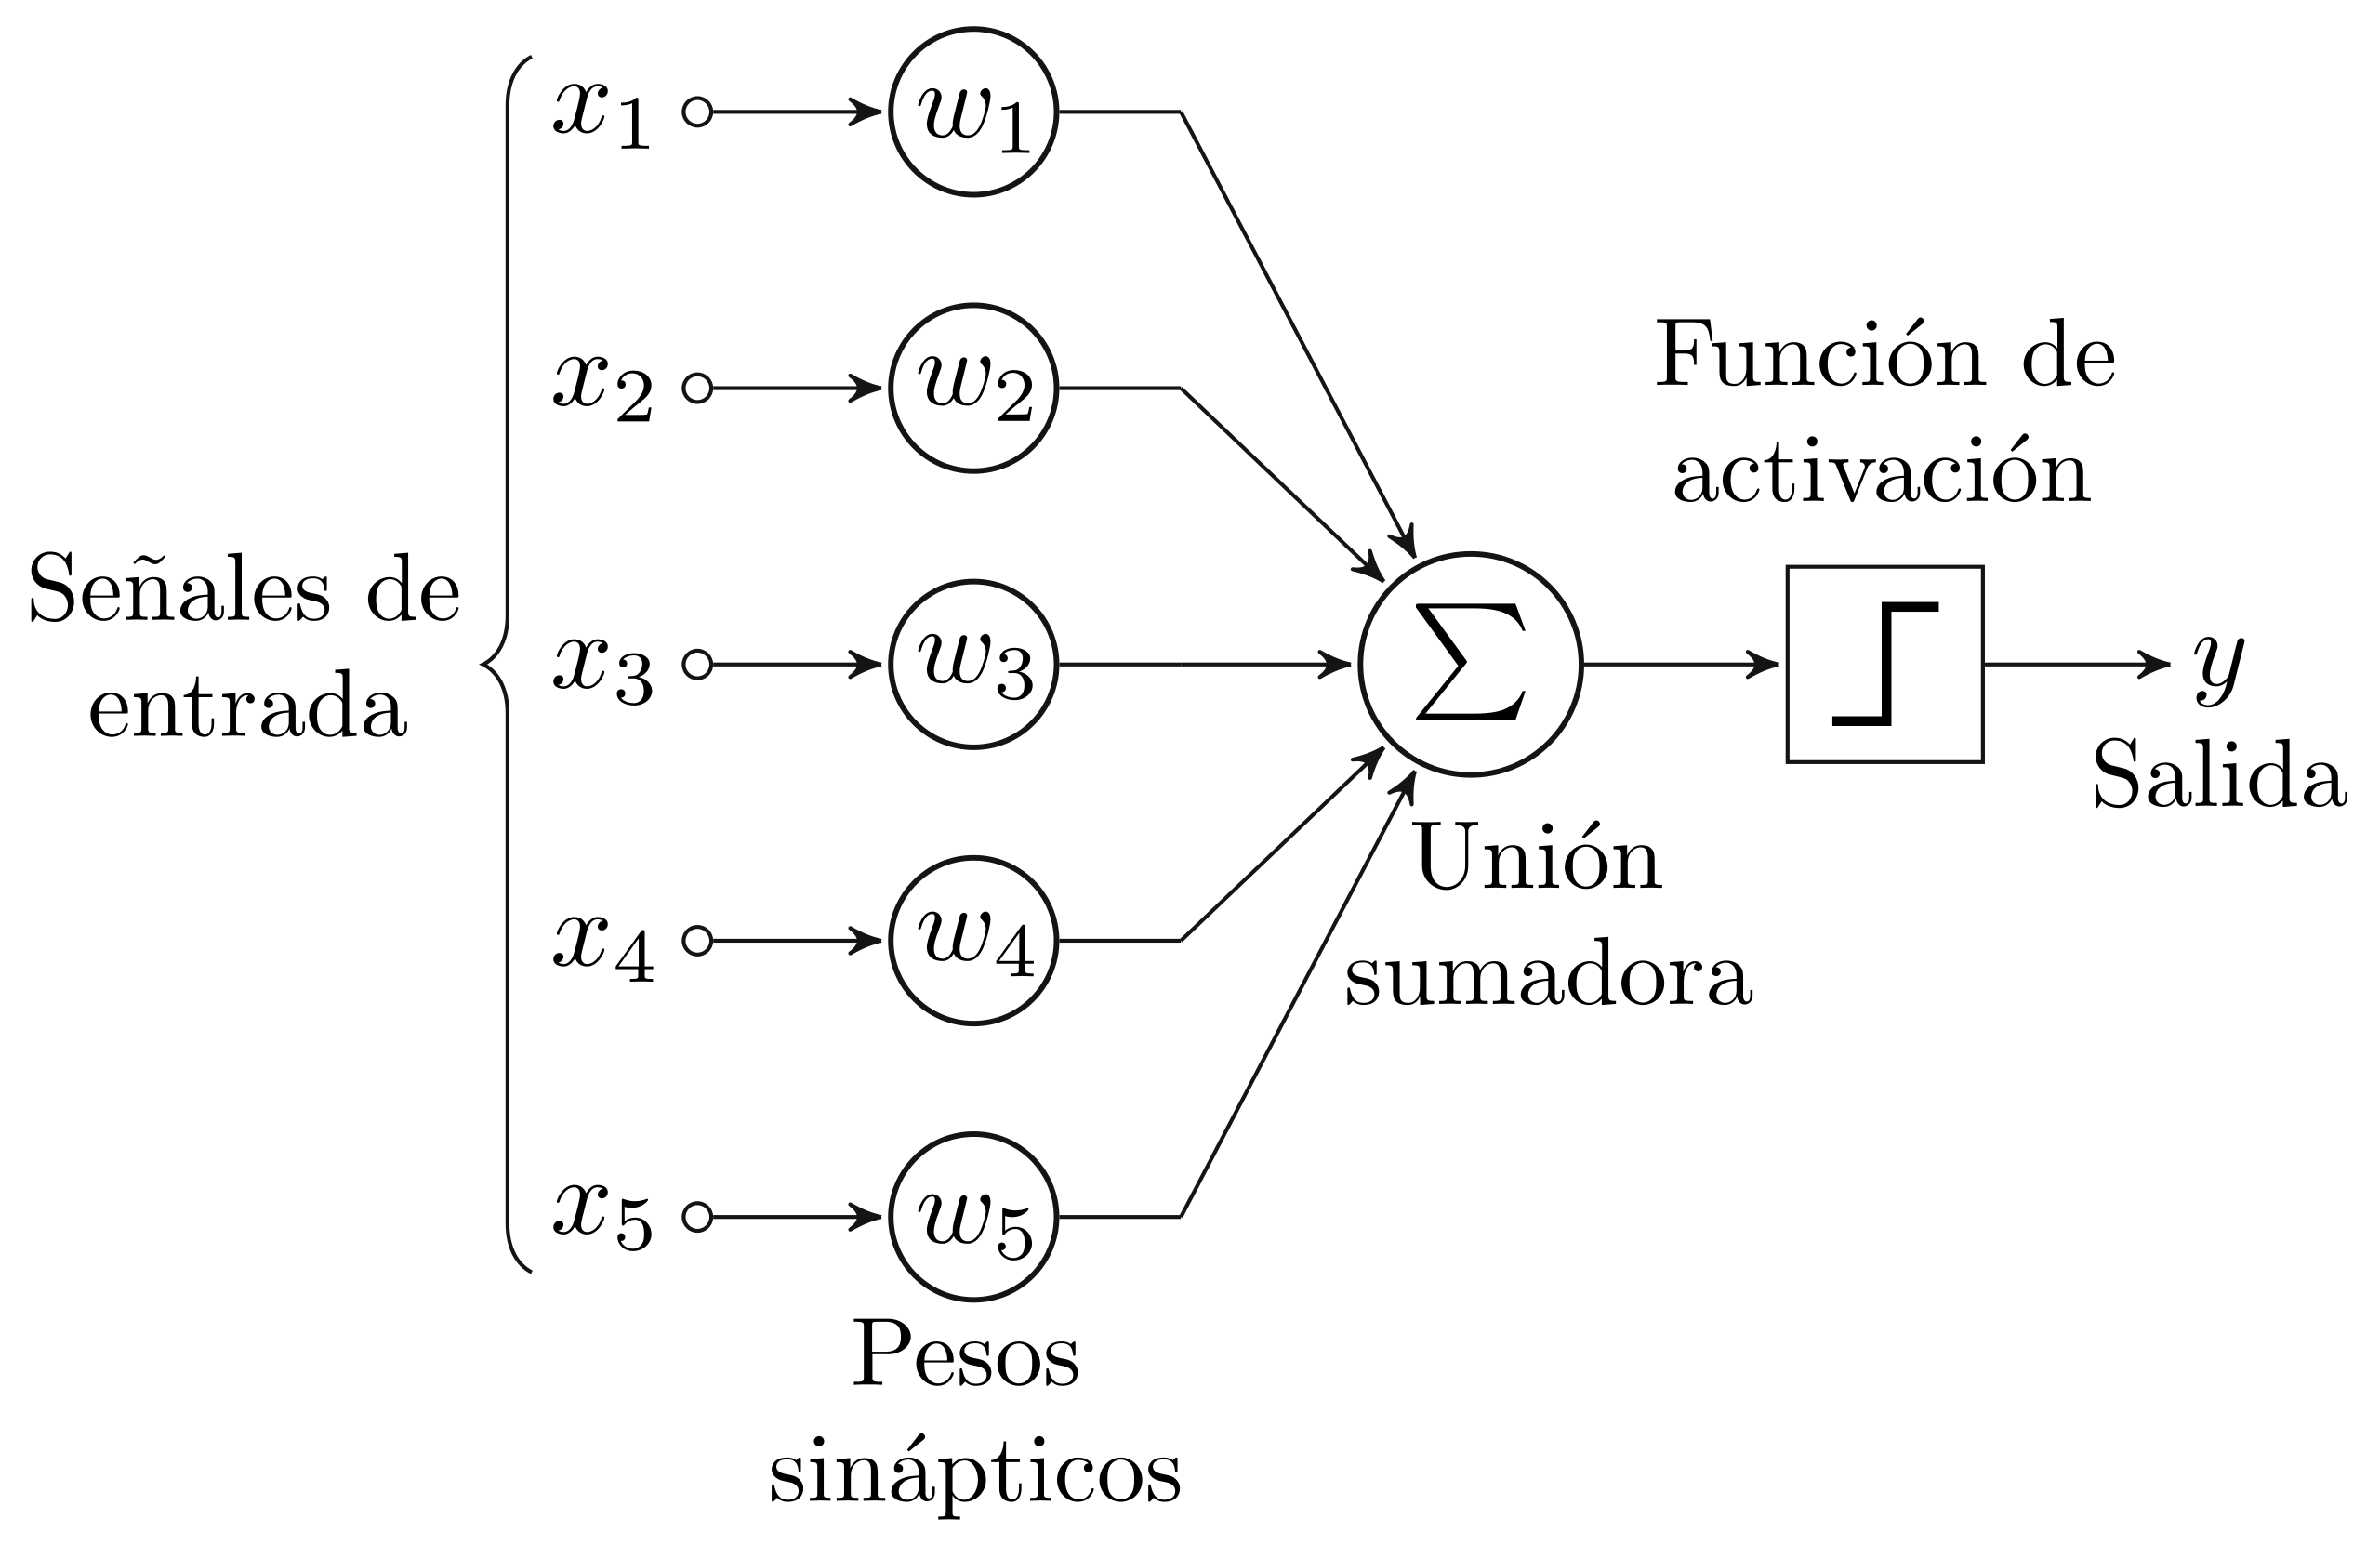
\includegraphics[width=0.8\linewidth]{Sem_1/figuras/Perceptron}
		\caption{Diagrama de un perceptrón con cinco señales de entrada \cite{imaPercep}.}
		\label{fig:diagrama_perceptron}
	\end{figure}
	En todo modelo de red neuronal artificial intervienen los siguientes elementos que conforman su estructura \cite{monsSistem}: 
	\begin{itemize}
		\item \textbf{Señales de entrada $(x_1, x_2,\dotsb,x_n)$:} pueden ser datos originales o provenientes de otras neuronas.
		\item \textbf{Señales de salida $(y_1,y_2,\dotsb,y_m)$:} que corresponde con los resultados de la red (clasificación o predicción en esta investigación).
		\item \textbf{Los pesos sinápticos $w_{1k},w_{2y},\dotsb,w_{nk}$:} A las entradas que provienen de otras neuronas se les asigna un peso, es decir, una determinada importancia. El peso es el numero que se modifica durante el entrenamiento de la red neuronal y que permite a la red adaptarse para conseguir la respuesta correcta.
		\item \textbf{Regla de propagación:} Se realizan diferentes operaciones con las entradas y los pesos. Con esto se busca obtener el valor del potencial que posteriormente se utilizara para realizar el procesamiento. Una de las operaciones más comunes es la suma ponderada. Otra regla puede ser la distancia euclidiana, que es utilizada por los mapas auto-organizados y las redes de función de base radial. 
		\item \textbf{La función de activación}: El valor obtenido en la regla de propagación se envía a través de la función de activación y esta define el nuevo estado o la salida de la capa. Según el entrenamiento de la red neuronal se elige la función de activación que pueden ser: lineal, escalón, sigmoidea, gaussiana o ReLU \cite{stephani}.
	\end{itemize}

	\subsection{Función de activación de las neuronas.}
	
	La función $o$ de la ecuación \ref{eq:percept} es la llamada función de activación. Para este tipo de redes, las funciones de activación más utilizadas son la la función tangente hiperbólica, función sigmoidal, y la función ReLU. Dichas funciones poseen como imagen un intervalo continuo de valores dentro de los intervalos $[-1,1]$ para la primera función antes mencionada y $[0,1]$ para las ultimas funciones antes mencionadas, estas vienen dadas por las siguientes ecuaciones: \\ \\
	\textbf{Función sigmoidal:}
	\begin{equation}
		\label{eq:tangente_hiper}
		f(x) = \frac{1}{1 + e^{-x}}
	\end{equation}
	\textbf{Función tangente hiperbólica:}
	\begin{equation}
		\label{eq:sigmoidal}
		f(x) = \frac{1-e^{-x}}{1 + e^{-x}}
	\end{equation}
	\textbf{Función ReLU:}
	\begin{equation}
		\label{eq:ReLU}
		\mathrm{ReLU}(x) = x^{+} = \mathrm{max}(0,x) = \frac{x + |x|}{2} = \left\{\begin{array}{lll}
			x & \text{si } x > 0, \\
			0 & \text{si } x \leq 0
		\end{array}\right.
	\end{equation}
	
		\begin{figure}[h]
		\centering
		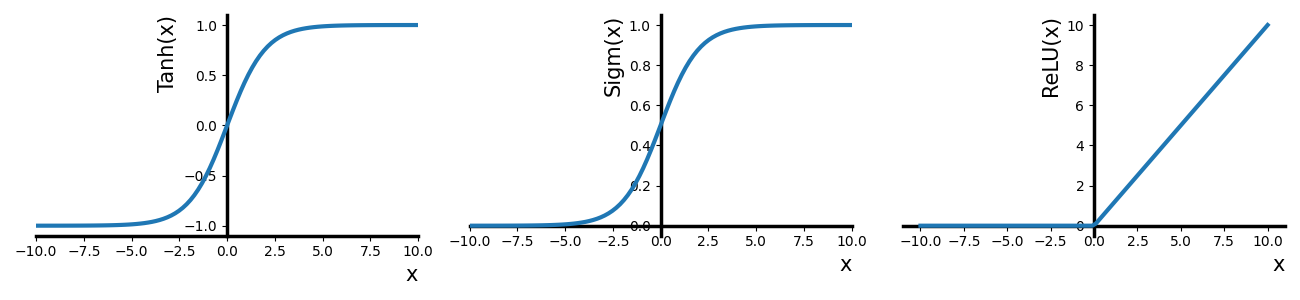
\includegraphics[width=0.9\linewidth]{Sem_1/figuras/funciones_de_activacion}
		\caption{Función tangente hiperbólica, función sigmoidal y función ReLU respectivamente.}
		\label{fig:funciones_activacion}
	\end{figure}
	
	En algunas ocasiones, la función de activación en el perceptrón multicapa es común a todas las neuronas de la red y es elegida por el diseñador, elección que se realiza unicamente basándose en los valores de activación que se desee que alcancen las neuronas. En otras ocasiones, y dependiendo de la naturaleza del problema, las neuronas de salida se distinguen del resto de neuronas de la red, utilizando otro tipo de función de activación \cite{percepMulti}.
	
	
	\subsection{El perceptrón multicapa.}
	Al combinar varios perceptrones dispuestos en forma de capas, se puede generalizar al perceptrón simple, este surgió como consecuencia de las limitaciones del mismo en lo referente al problema de separabilidad no lineal. Minsky y Papert mostraron en 1969 que la combinación de varios perceptrones simples podía resultar en una solución adecuada para tratar ciertos problemas no lineales. Sin embargo, los autores no presentaron una solución al problema de como adaptar los pesos de la capa de entrada a la capa oculta, pues la regla de aprendizaje del perceptrón simple no puede aplicarse a este escenario. No obstante, la idea de combinar varios perceptrones sirvió de base para estudios posteriores realizados por Rumelhart, Hinton y Williams en 1986 \cite{percepMulti}. Estos autores mostraron que una retropropagación de los errores medidos en la salida de la red hacia los perceptrones de las capas ocultas, dando lugar a la llamada regla delta generalizada. Diferentes autores han demostrado independientemente que el perceptrón multicapa es un aproximador universal, en el sentido de que cualquier función continua en un espacio $R^n$ puede aproximarse con un perceptrón multicapa, con al menos una capa oculta de neuronas \cite{stephani}.
 
 	Las características de las NN juegan un importante papel, por ejemplo, en el procesado de señales o imágenes. Se usan arquitecturas que comprenden elementos de procesado adaptativo paralelo, combinados con estructuras de interconexiones jerárquicas \cite{percepMulti}. Existen dos fases en la modelización con redes neuronales:
 	\begin{itemize}
 		\item \textbf{Fase de entrenamiento:} se usa un conjunto de datos o patrones de entrenamiento para determinar los pesos que definen el modelo de red neuronal. Se calculan de manera iterativa, de acuerdo con los valores de entrenamiento, con el objeto de minimizar el error cometido entre la salida obtenida por la NN y la salida esperada.
 		\item \textbf{Fase de prueba:} en la fase anterior, el modelo puede que se ajuste demasiado a las particularidades presentes en los patrones de entrenamiento, perdiendo su habilidad de generalizar su aprendizaje a casos nuevos.
 	\end{itemize}
 	
 	Las NN se pueden clasificar en diferentes formas dependiendo de los elementos básicos: según el número de capas pueden ser monocapa o multicapa. Según el tipo de retropropagación son recurrentes o no recurrentes. Según el mecanismo de aprendizaje supervisadas o híbridas. Según el tipo de conexión, totalmente conectadas o parcialmente conectadas.
 	
 	\subsection{Arquitectura.}
 	Existen 3 tipos de capas en un perceptrón multicapa, una capa de entrada, una capa de salida y una o mas capas ocultas.
 	\begin{enumerate}
 		\item \textbf{Capa de entrada:} son las encargadas de recibir la información de fuentes externas a la red, de aquí su nombre. En algunos casos, esta capa esta conectada a otras redes, las unidades de entrada reciben los datos de las salidas de las otras redes; en otros casos, simplemente reciben los datos que el usuario de la red introduce manualmente en el computador.
 		\item \textbf{Capas ocultas:} toda red mínimamente complicada, incluye este tipo de capa, estas no tiene relación directa con la información de entrada ni con la de salida, por lo que no son \guillemetleft visibles\guillemetright al ambiente exterior de la red, de ahí su nombre, su función es procesar la información en niveles más complejos para de esta forma hacer los cómputos más eficientes.
 		\item \textbf{Capa de salida:} Estas son las encargadas de dar la información al exterior, ofrecen la respuesta del sistema al usuario para su posterior tratamiento.
 	\end{enumerate}
 	\begin{figure}[h]
 		\centering
 		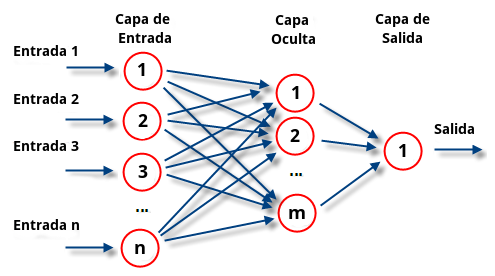
\includegraphics[width=0.7\linewidth]{Sem_1/figuras/RedNeuronalArtificial.png}
 		\caption{Arquitectura de un perceptrón multicapa con sus tres tipos de capas \cite{percMulti}.}
 		\label{fig:perceptron_multicapa}
 	\end{figure}
 	
 	En las NN las conexiones entre perceptrones siempre son hacia adelante, no existen conexiones laterales ni conexiones hacia atrás. Por tanto, la información siempre se transmite desde la capa de entrada hacia la capa de salida. Se considera $w_{ji}$ como el peso de conexión entre la neurona de entrada $i$ y la neurona de la capa oculta $j$, y $v_{kj}$ como el peso de conexión entre la neurona oculta $j$ y la neurona de salida $k$ \cite{percepMulti}. Los pesos óptimos se obtienen optimizando alguna función de energía. Por ejemplo, un criterio muy utilizado en el llamado entrenamiento supervisado, es minimizar el error cuadrático medio entre el valor de salida y el valor real esperado.
 	
 	\subsection{Algoritmo de retropropagación.}
 	Cuando se presenta un patrón $p$ de entrada $X_p : x_{p1},\dotsb,x_{pi},\dotsb,x_{pn}$, este se transmite a través de los pesos $w_{ji}$ desde la capa de entrada hacia la capa oculta. Las neuronas de la capa intermedia transforman las señales recibidas mediante la aplicación de una función de activación proporcionando, de este modo, un valor de salida. Este se transmite a través de los pesos $v_{kj}$ hacia la capa de salida, donde aplicando la misma operación que en el caso anterior, las neuronas de esta ultima capa proporcionan la salida de la red \cite{percepMulti,perceptron}.
 	
 	La regla de propagación más simple consiste en realizar la suma de las entradas ponderadas con sus pesos sinápticos correspondientes. Este proceso se resume en lo siguiente:
 	\begin{equation}
 		\label{eq:pesosxentrada}
 		h_{i(t)} = \sum_j w_{ij} \ast x_{j(t)}
 	\end{equation}
 	
 	\subsubsection{Etapa de aprendizaje.}
 	En esta etapa el objetivo es hacer lo mínimo el error entre la salida obtenida por la red y la salida deseada por el usuario ante la presentación de un conjunto de patrones denominado grupo de entrenamiento. Así, el aprendizaje en las redes de retropropagación es de tipo supervisado. La función de error que se pretende minimizar para cada patrón $p$ viene dada por:
 	\begin{equation}
 		\label{eq:error_a_minimizar}
 		e_p = \frac{1}{2}\sum_{k=1}^{M} (D_{pk} - Y_{pk})^2
 	\end{equation}
 	Se compara la salida obtenida $Y_p$ con la salida deseada $D_p$, donde $k$ en el índice de la neurona para las neuronas de la ultima capa, y $M$ el total de neuronas de la misma.
 	
 	A partir de esta expresión se puede obtener una medida general de error mediante: 
 	\begin{equation}
 		\label{eq:error_general}
 		e = \frac{1}{P} \sum_{p=1}^{P}e_p
 	\end{equation}
 	Siendo $p$ el índice de ejemplo, y $P$ el número total de ejemplos.
 	
 	La base del algoritmo de retropropagación para la modificación de los pesos es la técnica conocida como gradiente decreciente.
 	Como $e_p$ es función de todos los pesos de la red, el gradiente de $e_p$ es un vector igual a la derivada parcial de $e_p$ respecto a cada uno de los pesos. El gradiente toma la dirección que determina el incremento más rápido en el error, mientras que la dirección opuesta, es decir, la dirección negativa, determina el decremento más rápido en el error.
 	\begin{equation}
 		\label{eq:gradiente_error}
 		\Delta w_{ij} = -\alpha\frac{\partial e_p}{\partial w_{ji}}
 	\end{equation}
 	Si aplicamos la regla de la cadena a la ecuación \ref{eq:gradiente_error} obtenemos que:
 	\begin{equation}
 		\label{eq:gradiente_error_derivado}
 		\frac{\partial e_p}{\partial w_{ji}} = \frac{\partial e_p}{\partial h_j}\frac{\partial h_j}{\partial w_{ji}}
 	\end{equation}
 	La ecuación \ref{eq:gradiente_error_derivado} expresa la derivada del error en función de dos derivadas. La derivada del error respecto al potencial resultante $h_j$ indica como varia el error al variar la entrada de la neurona $j$, mientras que la derivada con respecto al peso sináptico $w_{ji}$ indica como varia la entrada de la neurona $j$ al variar el peso de la conexión que va desde la neurona $i$ hasta la neurona $j$.
 	
 	El segundo termino de la ecuación \ref{eq:gradiente_error_derivado} lo podemos expresar a partir de la ecuación \ref{eq:pesosxentrada} de la siguiente manera:
 	\begin{equation}
 		\label{eq:2dotermino_gradi_derivado}
 		\frac{\partial h_j}{\partial w_{ji}} = \frac{\partial \sum_i w_{ji} Y_{pi}}{\partial w_{ji}} = Y_{pi}
 	\end{equation}
 	Si escribimos el primer termino de la ecuación \ref{eq:gradiente_error_derivado} como:
 	\begin{equation}
 		\label{eq:1ertermido_gradi_derivado_reescrito}
 		\frac{\partial e_p}{\partial h_j} = -\delta_{pj}
 	\end{equation}
 	tenemos que
 	\begin{equation}
 		\label{eq:gradi_error_sustituido}
 		\frac{\partial e_p}{\partial w_{ji}} = -\delta_{pj}Y_{pi}
 	\end{equation}
 	y por lo tanto, la ecuación \ref{eq:gradiente_error} queda expresada de la siguiente manera
 	\begin{equation}
 		\label{eq:gradiente_error_reescrito}
 		\Delta w_{ji} = -\alpha\delta_{pj}Y_{pj}
 	\end{equation}
 	Para calcular el valor de $\delta$ se vuelve a aplicar la regla de la cadena
 	\begin{equation}
 		\label{eq:delta_pj_derivado}
 		\delta_{pj} = -\frac{\partial e_p}{\partial h_j} = - \left[\frac{\partial e_p}{\partial Y_{pj}} \frac{Y_{pj}}{\partial h_j}\right]
 	\end{equation}
 	El calculo del segundo termino de la ecuación \ref{eq:delta_pj_derivado} se hace por definición:
 	\begin{equation}
 		\label{eq:2dotermino_calculo_definicion}
 		\frac{\partial Y_{pj}}{\partial h_j} = \frac{f_j (h_j)}{\partial h_j} = f_j^{'}(h_j)
 	\end{equation}
 	Sin embargo, para el calculo del primer termino de la ecuación \ref{eq:delta_pj_derivado} es necesario distinguir entre dos casos diferentes. 
 	\begin{itemize}
 		\item \textbf{La neurona $j$ es una neurona de salida:} En este caso podemos obtener el segundo termino a partir de la ecuación \ref{eq:error_a_minimizar} ya que el subíndice $j$ es igual al subíndice $k$
 		\begin{equation}
 			\frac{\partial e_p}{\partial Y_{pj}} = \frac{\partial \frac{1}{2} \sum_{j=1}^{M} (D_{pj} - Y_{pj})^2}{\partial Y_{pj}} = -(D_{pj} - Y_{pj})
 		\end{equation}
 		Así, la variación de los pesos de una conexión que va hacia la capa externa de la red se calcula como:
 		\begin{equation}
 			\delta w_{ji} = \alpha(D_{pj} - Y_{pj}f_{j}^{'}(h_j)Y_{pi})
 		\end{equation}
 		\item \textbf{La neurona $j$ es una neurona oculta:} En este caso es necesario aplicar nuevamente la regla de la cadena 
 		\begin{equation}
 			\label{eq:error_neurona_oculta}
 			\frac{\partial e_p}{\partial Y_{pj}} = \sum_k \left[\frac{\partial e_p}{\partial h_k}\frac{\partial h_k}{\partial Y_{pj}}\right]
 		\end{equation}
 		Donde $k$ es el subíndice de las neuronas que pertenecen a la próxima capa. La ecuación \ref{eq:error_neurona_oculta} la podemos reescribir utilizando la ecuación \ref{eq:pesosxentrada}
 		\begin{equation}
 			\frac{\partial e_p}{\partial Y_{pj}} = \sum_k \left[\frac{\partial e_p}{\partial h_k} \frac{\partial\left[\sum_j w_{kj} Y_{pj}\right]}{\partial Y_{pj}}\right] = \sum_k \left[\frac{\partial e_p}{\partial h_k} w_{kj}\right]
 		\end{equation}
 		y por la ecuación \ref{eq:gradi_error_sustituido} tenemos que
 		\begin{equation}
 			\frac{\partial e_p}{\partial Y_{pj}} = \sum_k -\delta_{pk}w_{kj} = -\sum_k \delta_{pk}w_{kj}
 		\end{equation}
 		Así, la variación de los pesos de una conexión que va desde una capa hacia otra capa de la red que no sea la externa se calcula como:
 		\begin{equation}
 			\Delta w_{ji} = \alpha \sum_k (\delta_{pk}w_{kj}) f_j^{'}(h_j)Y_{pi}
 		\end{equation}
 	\end{itemize}
 	En la implementación del algoritmo, se toma una amplitud de paso que viene dado por la tasa de aprendizaje $\alpha$. A mayor tasa de aprendizaje el proceso será más rápido. Sin embargo, si la tasa de aprendizaje es muy alta puede dar lugar a oscilaciones en torno a un mínimo local. Es posible disminuir el impacto de dichas oscilaciones mediante la adición de un momento $\beta$ quedado la expresión \ref{eq:gradiente_error} de la siguiente manera:
 	\begin{equation}
 		\Delta w_{ji(t+1)} = \alpha \delta_{pj} Y_{pj} + \beta \Delta w_{ji(t)}
 	\end{equation}
 	De esta manera el momento $\beta$ determina el efecto en el instante $t+1$ del cambio de los pesos realizado en el instante $t$. Con este momento se consigue la convergencia de la red en menor número de iteraciones, ya que si la modificación de los pesos en los instantes $t$ y $t+1$ es en la misma dirección, entonces el descenso por la superficie de error en $t+1$ es mayor. En cambio, si la modificación en los pesos en los instantes $t$ y $t+1$ es más pequeño, lo que es adecuado, ya que esto significa que se ha pasado por un mínimo \cite{stephani}.
 	
 	\subsection{Dimensiones de la red.}
 	Una de las principales dificultades que surge a la hora de trabajar con redes neuronales, es la de seleccionar el número de capas y nodos por cada capa para que ésta funcione satisfactoriamente. El número de nodos en la capa de entrada suele venir determinado por la naturaleza del problema, el tamaño de la capa de salida es posible determinarlo decidiendo si se desean valores analógicos o binarios en las unidades de salida \cite{stephani}.
 	
 	En general, es suficiente que la red tenga tres capas, aunque a veces parece que un problema es más fácil de resolver con más de una capa oculta. Existen resultados experimentales que sugieren utilizar el menor número posible de unidades en las capas ocultas, y en caso de no lograr la convergencia de la red durante su entrenamiento, se debe aumentar el número de nodos hasta que se llegue a un tamaño final que logre el rendimiento global del sistema. Si al incrementar el número de nodos en una capa no se observan mejores en la convergencia de la red, es conveniente dividir esta capa en dos capas sucesivas \cite{perceptron}.
	\\ \\
	\textbf{Pesos de la red:} Los pesos de la red deberían recibir unos valores iniciales pequeños y aleatorios, generalmente entre $\pm$.\\ \\
	\textbf{Tasa de aprendizaje:} Controla el tamaño del cambio de los pesos en cada iteración. Se deben evitar dos extremos: un ritmo de aprendizaje demasiado pequeño puede ocasionar una disminución importante en la velocidad de convergencia y la posibilidad de acaba atrapado en un mínimo local; en cambio, un ritmo de aprendizaje demasiado grande puede conducir a inestabilidades en la función de error, lo cual evitara que se produzca la convergencia debido a que se darán saltos en torno al mínimo sin alcanzarlo \cite{nnApli,stephani}. Por tanto, se recomienda elegir un ritmo de aprendizaje lo más grande posible sin que provoque grandes oscilaciones. En general, el valor de la tasa de aprendizaje suele estar comprendida entre $0.01$ y $0.25$.
%\part{Segundo seminario}
\chapter{Marco Metodológico.}

\section{Enfoque general}
\subsection{Tipo de investigación.}

Esta tesis acoge un enfoque de investigación cuantitativa y experimental, donde se recopilan y procesan señales de electrocardiograma (ECG) de pacientes con diversas condiciones clínicas. Mediante técnicas avanzadas de aprendizaje automático no supervisado ---como el análisis de componentes principales (PCA), incrustación de vecinos estocásticos distribuidos en t (t-SNE)---, %y K-medios (K-means) 
que junto con las redes neuronales perceptrónicas (que serán los modelos predictivos) se busca identificar y clasificar patrones biomédicos específicos, a los que se denomina \emph{variables objetivo}.

\subsection{Diseño de la investigación.} \label{subsec:diseno_investigacion}
Esta investigación adopta un diseño predictivo longitudinal mediante el procesamiento de señales biomédicas provenientes de electrocardiogramas (ECG). En la primera etapa de este proyecto, se extraen atributos morfológicos y temporales, tales como los intervalos RR, complejos QRS, ondas P y T, entre otros, para esquematizar lo que será un vector de características multidimensional. Este canal habilita la aplicación de modelos de aprendizaje automático que, mediante algoritmos de reducción de dimensionalidad, clasificación y clustering\footnote{Agrupamiento de datos basados en la similitud}, identifican patrones no lineales y tendencias latentes en los datos. Los modelos se entrenan para dos objetivos, la clasificación de variables objetivo (grupos etarios, sexo y estado de salud, estas también denominadas \guillemetleft variables clínicas\guillemetright) y la identificación de integraciones biométricas basadas en rasgos cardíacos únicos. Aunque los métodos como las redes neuronales perceptrónicas operan como \guillemetleft cajas negras\guillemetright \ debido a su limitada interpretabilidad intrínseca, su robustez se garantiza mediante métricas de evaluación clínicamente relevantes, lo que permite asegurar generalización en datos no vistos por los modelos y sin que esto comprometa la confiabilidad predictiva.


\section{Diseño especifico}
\subsection{Flujo de procesamiento}

En la figura \ref{fig:diagrama_de_flujo_metodologico} se presenta un diagrama de flujo donde se especifican las 6 etapas para la adquisición y análisis de datos, las cuales son las siguientes:
\begin{enumerate}[label=\textbf{\Roman*.}]
	\item \textbf{Recopilación de los datos:} Se describe la fuente de las señales ECG, explicando brevemente el funcionamiento del banco de datos de Physionet y las bases de datos que se tomaron de ahí para este proyecto, a partir de ahí se eligen los criterios de selección de las señales electrocardiográficas y posteriormente, se aclara el formato en el que se guardaran las señales ECG para finalmente seleccionar la derivación \Romannum{2}.
	
	\item \textbf{Preprocesamiento de la señal ECG:} Se muestra la preparación previa de la data, ya homogenizadas las señales ECG a un mismo formato, se normaliza cada ECG de cada paciente para posteriormente filtrarlos y eliminar el desplazamiento de la linea base, teniendo cada señal limpia, se segmentan en intervalos de 3mín por cada señal ECG de cada paciente, luego con cada segmento se detectan los picos R para delimitar cada latido individual, teniendo estos latidos individuales alineados, teniendo los latidos alineados, se calcula un latido promedio por cada intervalo de cada paciente, este latido promedio será el vector de características que se usará más adelante.
	
	\item \textbf{Reducción de dimensionalidad:} Se inicia el calculo de la matriz de covarianza de los datos recogidos y la posterior obtención de los autovalores y autovectores, se procede a hacer el gráfico de suma de la varianza acumulada para determinar el numero optimo de componentes principales y se proyectan las señales ECG en el nuevo espacio creando un vector único de identificación, ya con esto se crea la base de conocimiento.
	
	\item \textbf{Modelado predictivo:} Se identifican las \guillemetleft variables objetivo\guillemetright \ las cuales fungirán como etiquetas \guillemetleft meta\guillemetright \ para las redes neuronales que se diseñarán y entrenarán en esta fase. Para cada una de las variables antes mencionadas, se diseña y entrena una red neuronal que sea capaz de clasificar e identificar a cada ECG dimensionalmente reducido que se usa como entrada en la red neuronal. Se entrena cada red, se obtienen las funciones de las redes que contienen los parámetros del entrenamiento, para su posterior guardado.
	
	\item \textbf{Análisis exploratorio:} Como etapa exploratoria, se aplicó t-SNE a las componentes principales para identificar agrupaciones supervisadas o no supervisadas en los ECG. Esto permitió validar que la reducción de dimensionalidad mediante PCA preserva información relevante y explorar la posible existencia de subpoblaciones de pacientes. Los resultados aportan evidencia sobre la viabilidad del uso de métodos no supervisados para descubrir dichas subpoblaciones ocultas.
	
	\item \textbf{Validación:} Se grafican las matrices de confusión y se calculan ciertas métricas de desempeño que expresen el rendimiento de cada red neuronal entrenada. Adicionalmente, con el fin de validar la capacidad de agrupamiento y discriminación de las representaciones obtenidas por las redes neuronales, se calculan las distancias de Mahalanobis entre las proyecciones dimensionalmente reducidas de las señales de ECG. Estos valores permiten analizar el grado de similitud y separación entre las distintas observaciones teniendo en cuenta la correlación existente en los datos. Posteriormente, se emplean estas distancias para la construcción de dendrogramas, ofreciendo una herramienta visual robusta que facilita la detección de posibles agrupaciones naturales dentro de la población estudiada. 
\end{enumerate}


	\begin{figure}[H]
		\centering
		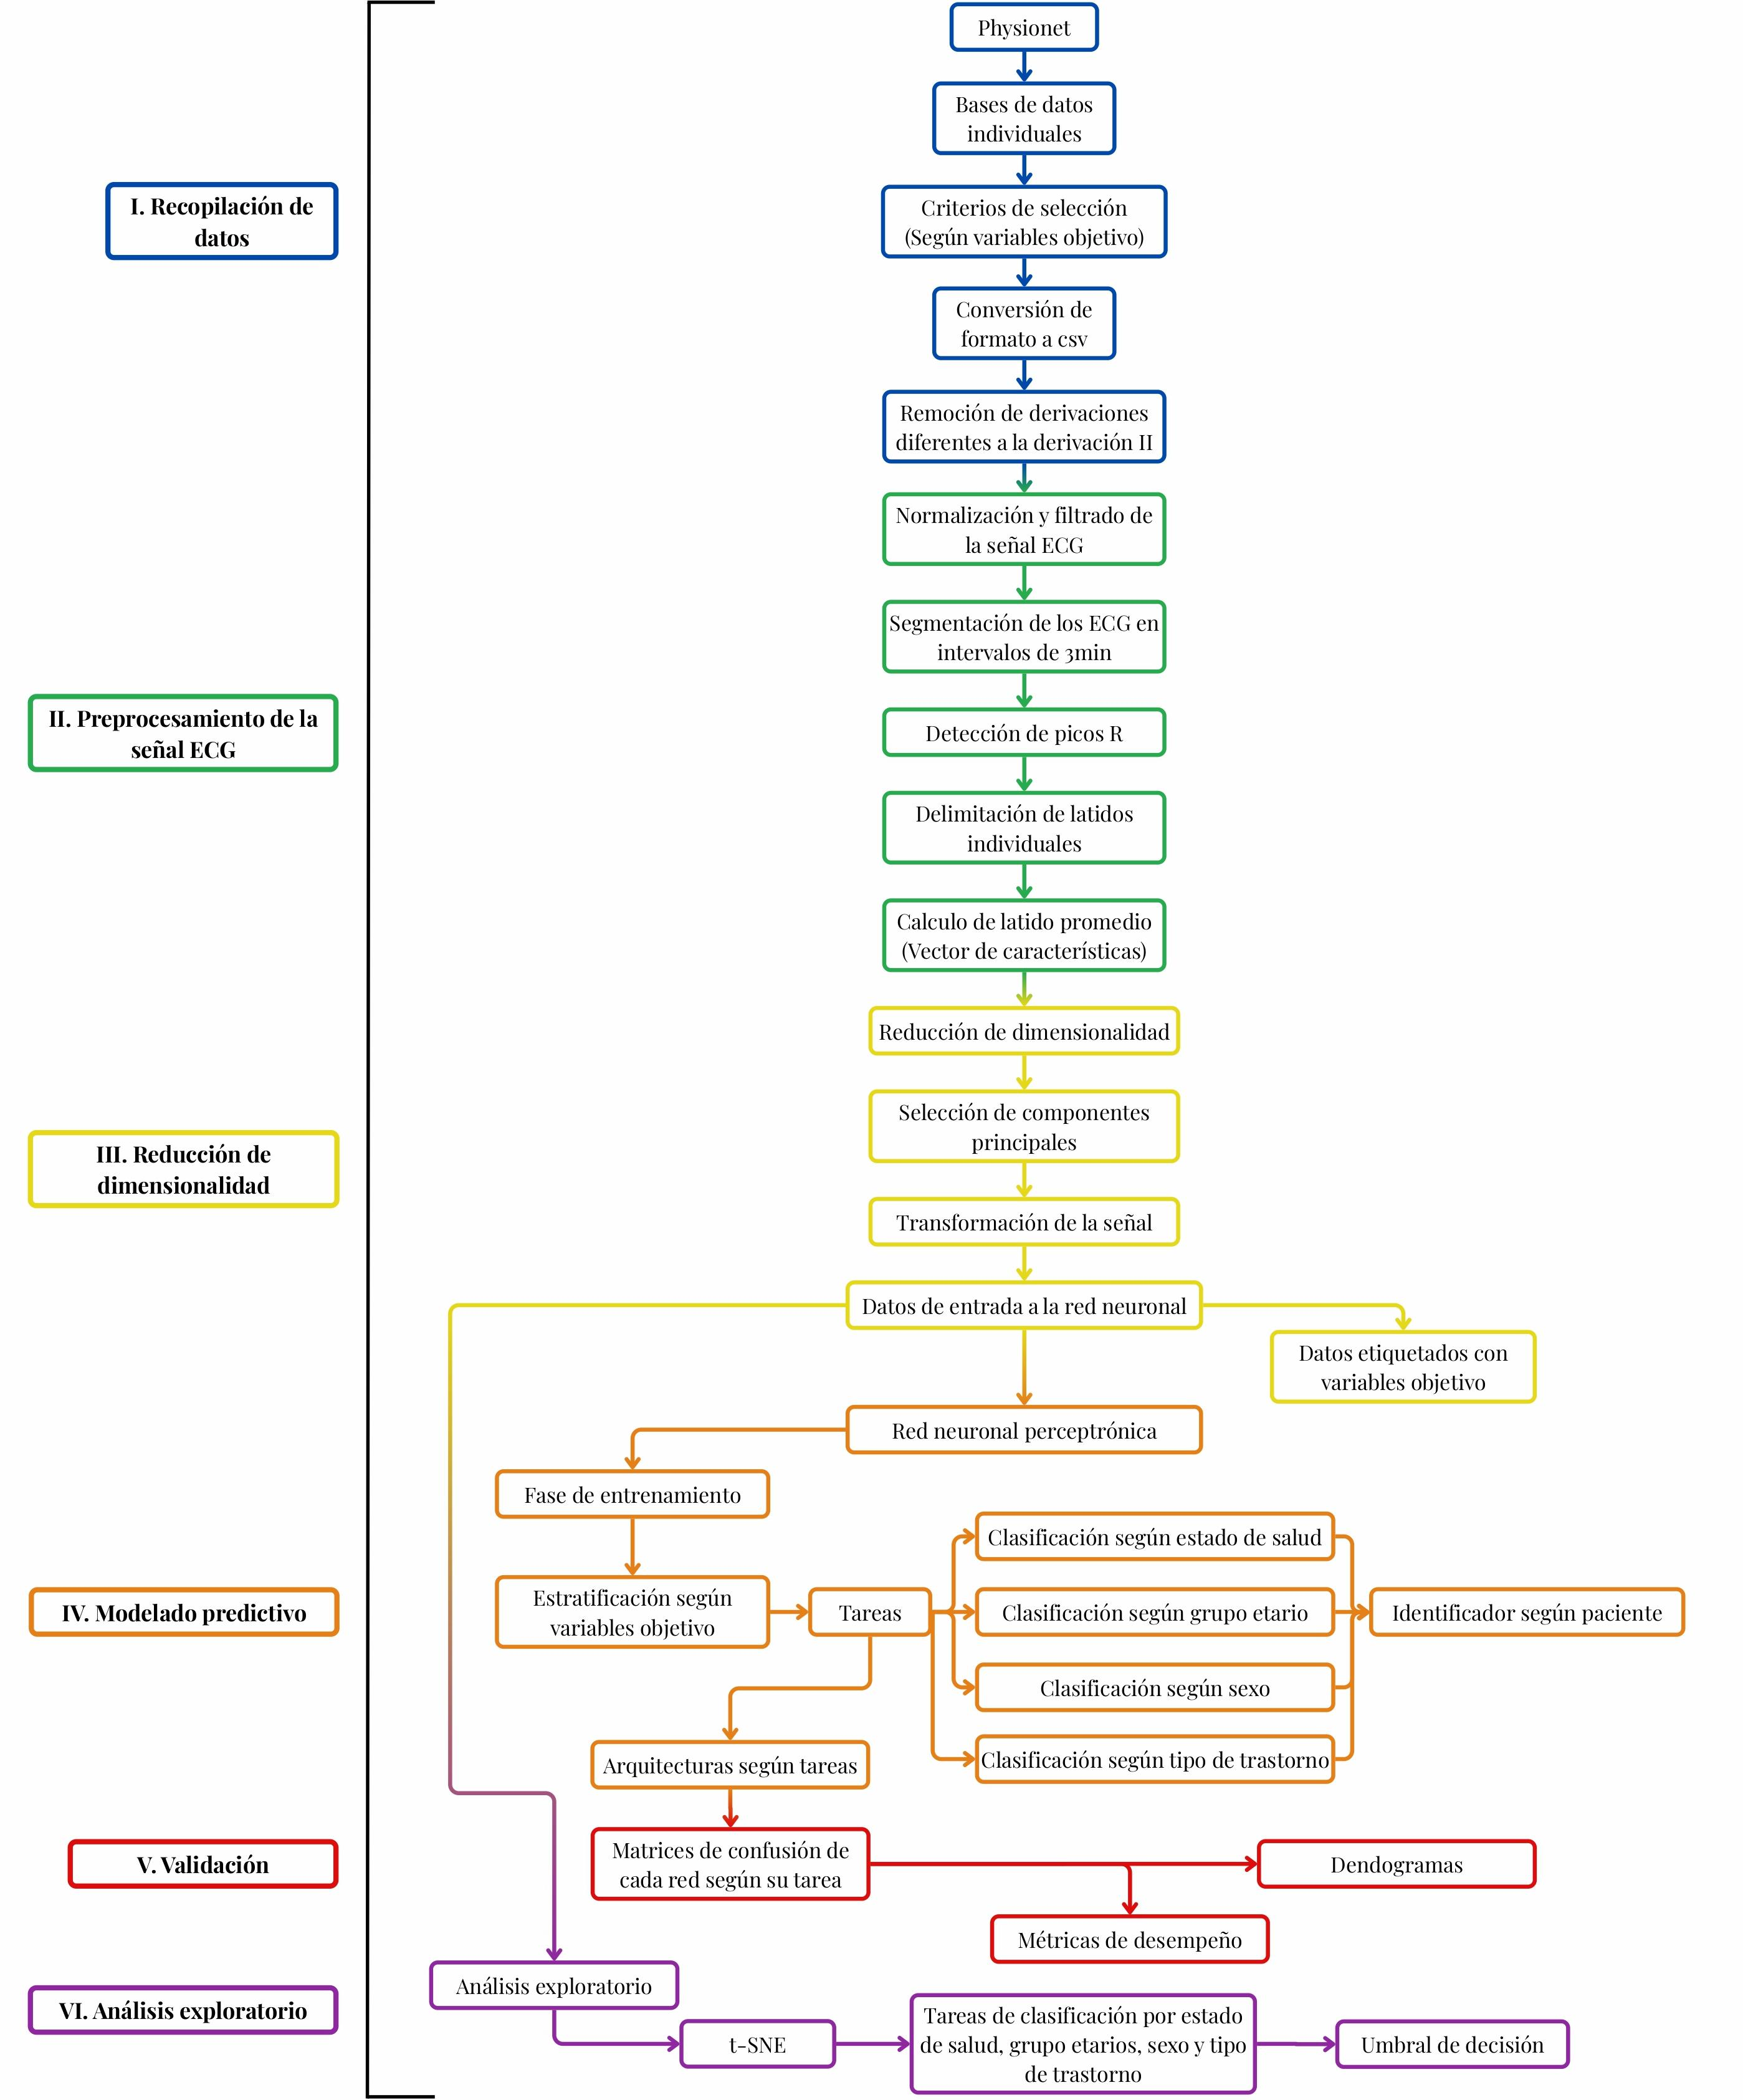
\includegraphics[width=1\linewidth]{Sem_1/figuras/Diagrama_de_flujo_metodologico.jpg}
		\caption{Diagrama de flujo que muestra un resumen desde la recopilación de los datos hasta la clasificación.}
		\label{fig:diagrama_de_flujo_metodologico}
	\end{figure}



\section{Población y muestra}

\subsection{Fuente de datos.}
Bajo los auspicios de los Institutos Nacionales de Salud (NIH, por sus siglas en inglés), que es la agencia principal del gobierno de los Estados Unidos responsable de la biomedicina y la salud publica de investigación, se creó en 1999, Physionet, bajo el apodo de \emph{Recursos de Investigación de Señales Fisiológicas Complejas}, siendo sus misiones originales y actuales, realizar y catalizar la investigación y la educación biomédica, en parte ofreciendo acceso gratuito a grandes colecciones de datos fisiológicos y clínicos y al software de código abierto relacionado. La plataforma Physionet es ahora administrada por miembros del Laboratorio de Fisiología Computacional del MIT. 

El recurso Physionet tiene tres componentes interdependientes:
\begin{itemize}
	\item Un extenso archivo (\guillemetleft PhysioBank\guillemetright) de grabaciones digitales bien caracterizadas y cuidadosamente revisadas de señales fisiológicas, series temporales y datos relacionados para uso de la comunidad de investigación biomédica. Physionet incluye colecciones de señales electrocardiográficas, cardiopulmonares, neuronales y otras señales biomédicas de sujetos sanos y pacientes con diversas afecciones con importantes implicaciones para la salud pública, como la muerte súbita cardíaca, la insuficiencia cardíaca congestiva, la epilepsia, los trastornos de la marcha, la apnea del sueño y el envejecimiento. Estas colecciones incluyen datos de una amplia gama de estudios, desarrollados y aportados por miembros de la comunidad investigadora. Physionet también incluye datos clínicos y de imagen relacionados con los cuidados críticos.
	\item Una amplia y creciente biblioteca de software (\guillemetleft PhysioToolkit\guillemetright) para el procesamiento y análisis de señales fisiológicas, la detección de eventos fisiológicamente significativos utilizando tanto técnicas clásicas como métodos novedosos basados en la física estadística y dinámica no lineal, la visualización interactiva y la caracterización de señales, la creación de nuevas bases de datos, la simulación de señales fisiológicas y de otro tipo, la evaluación cuantitativa y la comparación de métodos de análisis, y el análisis de procesos no estacionarios y de no equilibrio. 
	\item Una colección de tutoriales y materiales educativos populares, que ofrece orientación experta en enfoques para explorar y analizar datos sanitarios y señales fisiológicas. Un tema unificador de estos recursos es la extracción de información \guillemetleft oculta\guillemetright a partir de datos biomédicos, información que puede tener valor diagnostico o pronostico en medicina, o poder explicativo o predictivo en investigación básica.
\end{itemize}

Physionet no es solo el nombre los Recursos de Investigación de Señales Fisiológicas Complejas, es también un sitio web. Este sitio web fue creado como mecanismo de difusión y el intercambio gratuito y abierto de señales biomédicas grabadas y el software de código abierto para analizarlas, proporcionando instalaciones para el análisis cooperativo de datos y la evaluación de nuevos algoritmos. Además de proporcionar acceso electrónico gratuito a datos y programas informáticos, el sitio web de Physionet ofrece servicios y formación a través de tutoriales en linea para ayudar a los usuarios principiantes y avanzados. En colaboración con la conferencia anual \guillemetleft Computación en Cardiología\guillemetright, Physionet organiza una serie anual de desafíos, en los que investigadores y estudiantes abordan problemas no resueltos de interés clínico o científico básico utilizando datos y software proporcionados por Physionet \cite{physionet2000}.


\subsection{Criterios de selección.} 

Physionet ofrece un amplio banco de señales fisiológicas, en este proyecto estamos interesados en las bases de datos con señales electrocardiográficas, estas fueron seleccionadas considerando únicamente a aquellos que cumplían con:
\begin{itemize}
	\item Anotaciones de edad, sexo y estado de salud o diagnostico clínico de cada paciente al que se le registró el electrocardiograma, en el caso de pacientes sanos (pacientes de control), estos deben estar explícitamente etiquetados como tales en la base de datos.
	\item Tener al menos en unos de los canales de grabación, el registro de la derivación \Romannum{2} con una duración de al menos 15 minutos continuos, ya que esta será la señal que se usará de ahora en adelante.
\end{itemize}
Se excluyeron registros que no cumplían con los criterios antes mencionados. Además todas las señales usadas vienen del banco de señales fisiológicas de Physionet, ya que son señales provenientes de bases de datos públicas validadas, donde los registros cumplen con protocolos de adquisición y anotación médica impuestos por Physionet.

\subsection{Muestra} \label{subsec:muestra}
Se usaran señales provenientes de las siguientes bases de datos públicas presentes en Physionet: 
\begin{itemize}
	\item Apnea-ECG: La data consiste en 70 grabaciones que pueden variar en duración entre 7 y 10 horas cada uno, cada grabación tiene una señal ECG digitalizada, todos los pacientes tienen apnea del sueño \cite{apneaDB}. 
	\item Envejecimiento autonómico: Las funciones autonómicas del corazón como regular la presión arterial y el ritmo cardíaco disminuyen conforme aumenta la edad, el estudio que produjo esta base de datos provee señales biológicas de alta resolución para describir el efecto del envejecimiento sano en la regulación cardiovascular. Señales electrocardiográficas y de presión arterial continua no invasiva fueron grabadas en reposo a 1120 voluntarios sanos, a los cuales se les practicaron pruebas rutinarias de laboratorio y cuyos resultados no arrojaran hallazgos patológicos, excluyendo a aquellos pacientes que tuvieran condiciones medicas, consumo de drogas ilegales o medicamentos que potencialmente pudieran influir en el funcionamiento cardiovascular \cite{autonomicAgingDB}.
	\item BIDMC Insuficiencia cardíaca congestiva: Esta base de datos incluye grabaciones de larga duración de 15 pacientes con insuficiencia cardíaca congestiva severa (NYHA\footnote{Clasificación del grado de insuficiencia cardíaca según la Asociación del Corazón de Nueva York} clase 3 o 4) \cite{InsuficienciaCardiacaDB}
	\item Fantasía: Es una base de datos de señales electrocardiográficas de 120 minutos cada una de 40 pacientes sanos rigurosamente seleccionados y calificados como pacientes sanos, estos sujetos permanecieron en estado de reposo y ritmo sinusal normal mientras veían la película Fantasía (Disney, 1940) con el fin de mantenerse en vigilia \cite{fantasiaDB}.
	\item Arritmia (MIT-BIH Arritmia DB): Es un conjunto de 48 grabaciones de señales electrocardiográficas de dos canales, siendo una de estas siempre la derivación \Romannum{2}, de media hora de duración cada una, fue una de las primeras bases de datos disponibles en Physionet y es una de las bases de datos más usadas como material de prueba para detectores de arritmia \cite{arritmiadb}. 
	\item ECGs de larga duración: Esta es una colección de 7 grabaciones electrocardiográficas de larga duración (entre 14 y 22 horas cada uno), con anotaciones manuales de los tipos de latidos extraños presentes en cada grabación. Esta base de datos fue desarrollada para apoyar la investigación en el campo de la detección de las arritmias cardíacas y sus análisis, los pacientes de los registros no son pacientes sanos \cite{longtermdb}.
	\item Ritmo sinusal normal: Esta base de datos incluye 18 grabaciones de larga duración de electrocardiograma de pacientes referidos del Laboratorio de arritmias del Beth Israel Hospital (BIH) de Boston. Se comprobó que los sujetos incluidos en esta base de datos no presentaban arritmias significativas, por lo que es de destacar, que estos pacientes están considerados como pacientes sanos por al menos 2 cardiólogos \cite{normalsinusrhythmdb}. 
	\item La base de datos polisomnográficos (MIT-BIH Polysomnographic Database) es una colección de grabaciones de múltiples señales fisiológicas durante el sueño, entre ellas, se tiene la derivación \Romannum{2} de cada grabación de cada paciente. Cada uno de estos pacientes fueron monitorizados en el Laboratorio de Sueño del BIH de Boston para evaluar el síndrome de apnea obstructiva crónica del sueño y comprobar los efectos de la presión positiva constante en las vías respiratorias, una intervención terapéutica estándar que suele prevenir o reducir sustancialmente la obstrucción de las vías respiratorias en estos sujetos \cite{polysomnogradb}.
%	\item Base de datos de electrocardiogramas de 12 derivaciones a gran escala para el estudio de arritmias: Esta colección fue creada bajo los auspicios de la Universidad de Chapman, el hospital de la gente de Shaoxing y el primer hospital de Ningbo. Posee mas de cuarenta y cinco mil grabaciones de 10 segundos de duración de las 12 derivaciones de un electrocardiograma, este paquete de señales puede utilizarse para diseñar y comparar y poner a punto técnicas estadísticas clásicas y de aprendizaje automático nuevas y clásicas en estudios centrados en la arritmia y otras afecciones cardiovasculares \cite{largeescale12leaddb}. PONER ESTO SI Y SOLO SI SE USA ESTA BASE DE DATOS
	
\end{itemize}
Los ECG provenientes de las bases de datos antes mencionadas, están distribuidos como se muestra en la tabla \ref{tab:distriECGs}, según las variables objetivo tomadas de los criterios antes mencionados. 
Es de destacar también que todas las señales fisiológicas disponibles en Physionet han sido guardadas en un formato estandarizado por ellos mismos, además ponen a disposición una librería en Python, llamada \emph{Waveform Database Software Package (WFDB) for Python} \cite{wfdb}, la cual permite transformar las señales a formatos más universales como, archivos separados por comas (CSV, por sus siglas en inglés). Cabe señalar que, aunque las bases de datos utilizadas están disponibles a través de Physionet, estas no provienen todas del mismo instituto de investigación o universidad. Como consecuencia, los profesionales de la salud encargados de catalogar y diagnosticar a los pacientes, varían entre una base de datos y otra, lo que pudiera introducir cierto grado de subjetividad en las anotaciones clínicas asociadas de la muestra a estudiar.

\begin{table}[ht]
	\renewcommand{\arraystretch}{2}
	\begin{center}
		\begin{tabular}{|p{1.85cm}|M{1.7cm}|M{1.55cm}|M{1.15cm}|M{2.2cm}|M{1.5cm}|M{1.5cm}|M{1.5cm}|M{1cm}|}
			\hline
			& \textbf{Hombres} & \textbf{Mujeres} & \textbf{Sanos} & \textbf{Patológicos} & \textbf{Adultos Jóvenes} & \textbf{Adultos de Mediana Edad} & \textbf{Adultos Mayores} & \textbf{Total} \\
			\hline
			\textbf{Cantidad de Pacientes} & \centering352 & 410 & 611 & 151 & 435 & 222 & 106 & 762 \\
			\hline
		\end{tabular}
		\caption{Distribución de ECGs con los pacientes seleccionados para el estudio.}
		\label{tab:distriECGs}
	\end{center}
\end{table}


\section{Preprocesamiento de la señal}
	
Para garantizar la confiabilidad de los posteriores análisis es critico el preprocesamiento de las señales electrocardiográficas. Debido a la naturaleza digital de los ECG que se tienen, se aprovecha el lenguaje de programación \emph{Python} que cuenta con ventajas tales como una gran comunidad que apoya constantemente en la resolución de problemas y el desarrollo de librerías entre las que destacan las diseñadas para el análisis de datos y algunas más específicas como las que permiten analizar datos fisiológicos, de acá radica parte de la importancia de elegir a \emph{Python} como lenguaje base en esta investigación. Las señales adquiridas de las bases de datos antes mencionadas no están exentas de los ruidos inherentes a la adquisición de la misma estas suelen contener artefactos y demás tipos de ruidos que es necesario eliminar, es por esto que se implementa un flujo de preprocesamiento estructurado en cinco etapas principales:
\begin{enumerate}
	\item \textbf{Estandarización de la señal:} En el análisis de datos, la estandarización es una de las herramientas básicas y comúnmente utilizadas, existen varios tipos y dependerá de los datos cual usar.
	\item \textbf{Filtrado de ruido:} Es necesario reducir o eliminar el ruido provocado por la actividad muscular y la interferencia de la red eléctrica, para esto se usan filtros digitales (Butterworth, por ejemplo) con frecuencias de corte ajustadas a las bandas típicas del ECG.
	\item \textbf{Eliminación del desplazamiento de la linea base:} también conocido como \emph{baseline wander}, es un ruido de baja frecuencia ($<0.5\ Hz$) que distorsiona la morfología del ECG llegando a afectar la detección de las ondas P y T. Para esto se aplica el algoritmo de Sharma \& Sharma \cite{Sharma15} para preservar la morfología real del ECG.
	\item \textbf{Extracción de segmentos ECG:} Debido a que el algoritmo propuesto por Sharma \& Sharma \cite{Sharma15} se desempeña mejor conforme más largo es el segmento a ser tratado por el mismo, se extraen los segmentos de los ECG (de duración fija) luego de haber sido filtrados y que haya sido eliminado el desplazamiento de la linea base. Para homogenizar el análisis, se selecciona una duración fija de 3 minutos, que permitan equilibrar la captura de la variabilidad de los latidos cardíacos. 
	\item \textbf{Detección de eventos cardíacos:} Seleccionando algoritmos basados en el robusto algoritmo de Pan-Tompkins \cite{PanTompkins85} se busca la identificación precisa de los complejos QRS (picos R) como referencia temporal de cada latido.
\end{enumerate}

\subsection{Estandarización}

La estandarización de los datos se suele hacer por dos razones:
\begin{enumerate}
	\item Cada electrocardiógrafo digitaliza la señal ECG a diferente factor de conversión analógico-digital (ADC) ---lo que resulta en señales con escalas dinámicas diferentes, es decir, valores en mV representados con rangos numéricos distintos--- por lo que se requiere regularizar las escalas dinámicas de los datos.
	\item La linea base de la señal ECG suele no estar situada en el centro común del papel milimetrado donde queda grabada la señal, es por esto que se debe eliminar el \emph{offset}\footnote{Se refiere al desplazamiento en la señal producto de un voltaje constante propio del instrumento que se suma a la señal que se busca medir} del instrumento y así centrar la linea base del ECG.
\end{enumerate}
Entre los distintos tipos de regularización de datos existentes, es importante señalar que el uso de cada tipo de regularización dependerá de los datos y del problema a solucionar, en esta investigación se usará la siguiente transformación lineal:
\begin{equation}
	\label{eq:normalizacion}
	\mathrm{X}=\frac{\mathrm{x}-\overline{\mathrm{x}}}{\sigma}
\end{equation}
siendo $\mathrm{X}$ el nuevo vector de datos estandarizado, $\mathrm{x}$ la variable de entrada, $\overline{\mathrm{x}}$ su valor medio y $\sigma$ la desviación estándar. Este tipo de regularización tendrá valor medio cero y la desviación estándar igual a uno, con lo que se evitaran tendencias de las entradas fuera de los rangos considerados como normales, debido a los desplazamientos de la linea base de la señal. Por otra parte su uso preserva la estructura original de los datos lo que permite que las correlaciones se mantengan, siendo esto lo apropiado para posteriores algoritmos como PCA y redes neuronales.
\subsection{Filtrado de ruido}

Para la etapa de filtrado, es necesario identificar la banda que maximice la energía del QRS, siendo esta ($0.5 - 15 \ Hz$) \cite{PanTompkins85}, posteriormente se diseña un filtro digital tipo Butterworth de orden 10 y tipo pasabanda usando el corte de bandas antes mencionado. La rapidez de este tipo de filtrado permite que pueda ser implementado en tiempo real dejando suficientes recursos computacionales para posteriores tareas. 

\subsection{Remoción del desplazamiento de la línea base}

El desplazamiento de la línea base (BW, por sus siglas en inglés) del electrocardiograma es causado principalmente por el movimiento y el proceso respiratorio del paciente lo que hace que aparezcan artefactos de baja frecuencia de las señales ECG. Para una mejor visualización e interpretación es necesario remover el BW, esto permite que posteriores procesos de detección de eventos cardíacos y subsecuentes procesos de automatización sean eficaces. Si bien el BW es una señal de baja frecuencia, el uso de un filtrado paso alto no es recomendable ya que puede distorsionar la morfología del ECG ya que causa variaciones en el espectro de frecuencias de la señal ECG, es por esto que se sugiere emplear técnicas que puedan remover el BW sin deformar la señal ECG. La descomposición vibracional de Hilbert (HVD, por sus siglas en inglés) propuesta por Sharma \& Sharma en 2015 \cite{Sharma15} es una método que extrae las mono-componentes de una señal usando su forma analítica donde las primeras componentes corresponden a las más altas amplitudes instantáneas. Las componentes con las amplitudes instantáneas más altas hacen referencia a la componente dominante de la señal. La HVD estima esta mayor componente de energía como una función media de las frecuencias instantáneas (IF) de la composición, es decir, esta técnica es un método iterativo en el que cada iteración incluye los tres pasos siguientes: 
\begin{enumerate}
	\item Estimación de la IF de la componente mayor (la más baja frecuencia encontrada).
	\item Extracción de la envolvente correspondiente de la componente mayor. 
	\item Sustracción de la componente mayor de la señal compuesta.
\end{enumerate}
Por lo tanto, la señal original $x(t)$ puede representarse como una suma de diferentes mono-componentes con amplitudes y frecuencias instantáneas que varían lentamente. Así, utilizando la técnica HVD, la señal $x(t)$ puede expresarse como: 
\begin{equation}
	x(t) = \sum_k a_k(t)\cos\left( \int \omega_k(t)dt\right)
	\label{eq:senal_HVD}
\end{equation}
donde $a_k(t)$ y $w_k(t)$ son las amplitudes instantáneas y la IF del k-ésimo componente respectivamente \cite{Sharma15}. 
En esta investigación, usando la técnica de la descomposición vibracional de Hilbert, se sustrae la primera componente de la señal ECG original que es:
\begin{equation}
	x_1(t) = a_1(t)\cos \left(\int \omega_1(t)dt \right)
	\label{eq:baseline_wander}
\end{equation}
esta corresponde con el desplazamiento de la linea base. Por consiguiente, la señal residual $x^{\prime}(t)$ es la combinación de las demás componentes de más bajas amplitudes que resultan ser la señal original sin los artefactos introducidos por el desplazamiento de la linea base y sin cambios en la morfología original de la misma, dicho de otra manera, la señal ECG con la linea base corregida es obtenida sustrayendo el BW de la señal ECG original, esto es:
\begin{equation}
	x^{\prime}(t)=x(t)-x_1(t)
	\label{eq:senal_sin_bw}
\end{equation}
Esta técnica se desempeña mejor conforma la señal sea más prolongada, es por esto que esta remoción de la linea base se hace previo a la segmentación de la señal ECG en intervalos de tiempo más cortos. Como se puede observar en la figura \ref{fig:remocion_bw}, la HVD es capaz de mantener la morfología real del ECG mientras elimina cualquier artefacto de baja frecuencia que haga variar la linea base.
\begin{figure}[h]
	\centering
	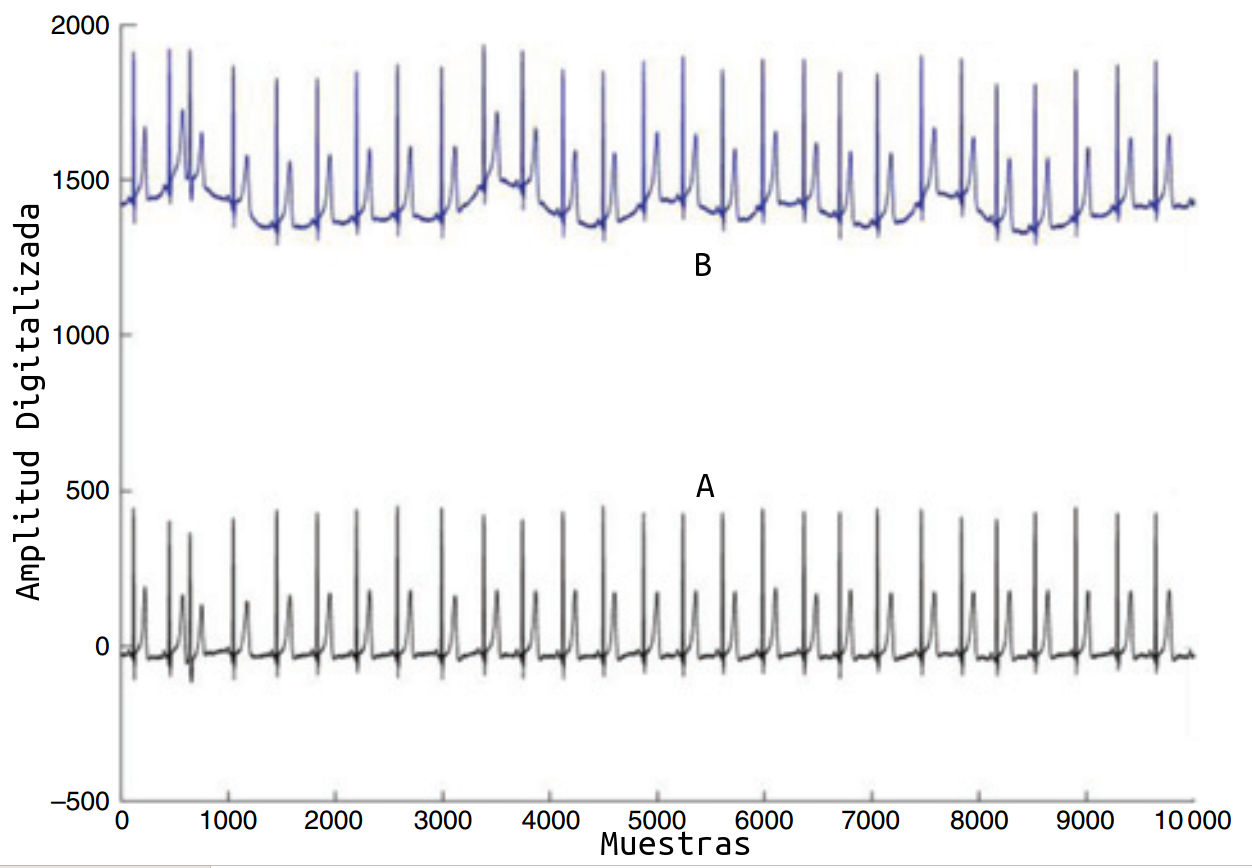
\includegraphics[width=0.85\linewidth]{Sem_1/figuras/Baseline Wander Sharma.png}
	\caption{Remoción del desplazamiento de la línea base usando la técnica HVD \cite{Sharma15}.
		A) Señal ECG con BW artificial de 900 de amplitud. 
		B) Señal ECG $x^{\prime}(t)$ con la línea base corregida.}
	\label{fig:remocion_bw}
\end{figure}
 	
\subsection{Extracción de segmentos}

Debido a que las señales ECG que se tienen, son señales con duraciones mayores a 20 minutos, se pensó en aumentar la cantidad de señales segmentando cada una de estas en intervalos de 3 minutos con la finalidad de tener más registros del mismo paciente. Así que luego que cada señal haya sido filtrada y tenga la linea base corregida, se segmentó y separó la señal en intervalos de 3 minutos, hasta tener como máximo 10 señales de 3 minutos de duración de cada paciente.

\subsection{Detección de eventos cardíacos}

Es importante recordar que cada latido visto en el ECG está compuesto por ondas individuales, de las cuales se puede extrapolar el funcionamiento de cada parte del corazón mientras este se contrae y se relaja, es por esto que resulta clave poder detectar los eventos relevantes del latido, tales como el pico R, el inicio de la onda P o el final de la onda T. Para detectar dichos eventos se ha hecho uso de distintas técnicas, donde cada una de estas se desempeña mejor dependiendo del tipo de evento a localizar. Por ejemplo, el algoritmo Pan-Tompkins \cite{PanTompkins85} fue el primero y uno de los mejores computacionalmente hablando para detectar los picos R, sin embargo, hoy en día se han mejorado estos algoritmos aumentando su eficiencia y reduciendo el costo computacional al mismo tiempo, aunque estos están basados en la aproximación hecha por Pan-Tompkins. 

Con el fin de aprovechar las herramientas hechas por la comunidad científica, en la presente investigación se hace uso de la librería \emph{Neurokit2} \cite{neurokit21}, este paquete provee rutinas de procesamiento avanzado de bioseñales que permiten a investigadores y médicos, analizar datos fisiológicos de manera sencilla y sin necesidad de poseer conocimientos extensivos en procesamiento de señales biomédicas y programación. Esta librería, está enfocada en todo lo que involucra el análisis de señales fisiológicas siendo una de estas, las señales ECG y entre las muchas funcionalidades presentes en esta librería, se hace uso de detector de picos R propuesto y usado en esta, este a su vez, esta basado en el algoritmo llamado \emph{Biopeaks} \cite{biopeaks_software20} propuesto por Jan C. Brammer en 2020, este algoritmo presentó una precisión del $99.95\%$ en la detección de picos R \cite{Biopeaks20} siendo este, uno de los algoritmos más eficientes hoy en día, para la localización de eventos cardíacos como los picos R, de aquí que haya sido empleado en este trabajo. En la figura \ref{fig:ecg_delimitado} se observa un ejemplo de ECG con los latidos individuales delimitados y los picos R debidamente localizados.

\begin{figure}[h]
	\centering
	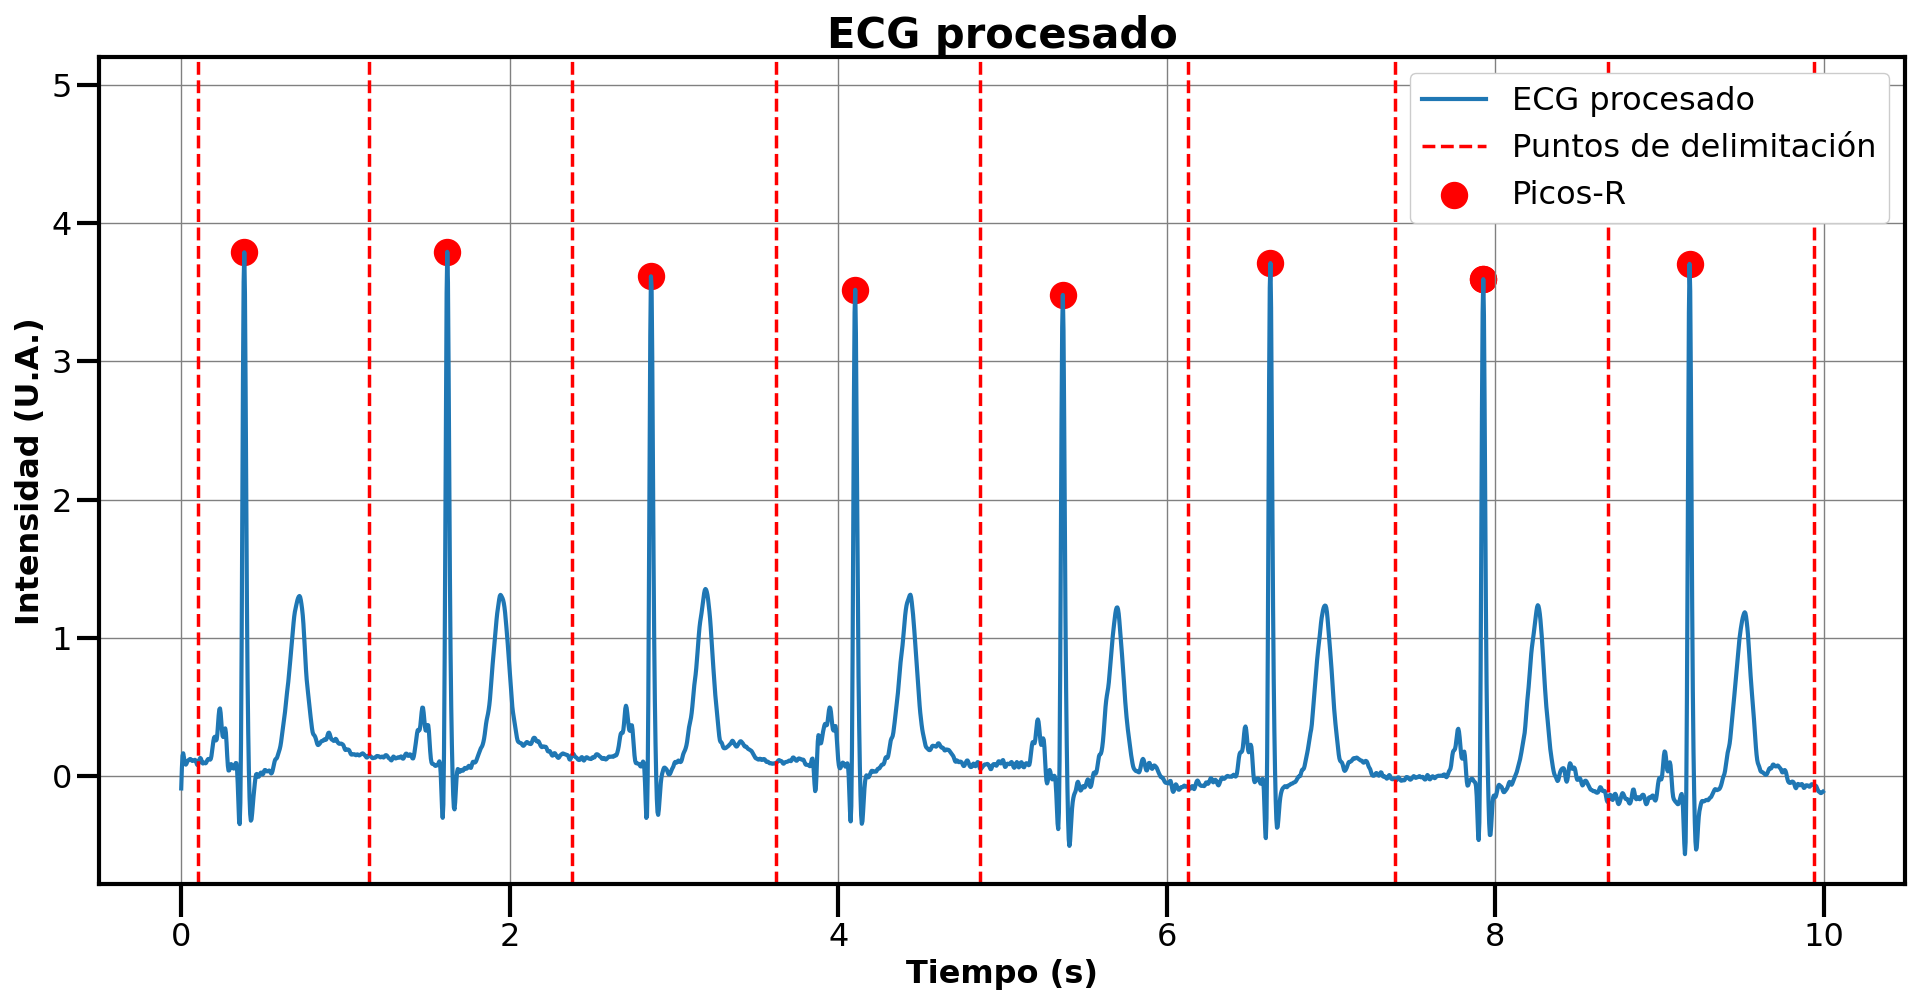
\includegraphics[width=0.85\linewidth]{Sem_1/figuras/ECG_procesado_10s_delimitado.png}
	\caption{ECG procesado con latidos individuales delimitados y picos R localizados.}
	\label{fig:ecg_delimitado}
\end{figure}

\section{Extracción de características}

Es relevante recordar que PCA necesita como entrada un vector con las características claves de conjunto de datos a analizar. En el caso de las señales ECG, extraer características recae fundamentalmente en la habilidad de detectar correctamente los inicios, picos y finales de las ondas individuales de cada latido, teniendo estos puntos debidamente localizados se podrían calcular los intervalos PR y QT; y los segmentos PR y ST como se observan en la figura \ref{fig:ECGSinusal}, y teniendo los promedios de estos valores, se podría construir un vector de características de cada paciente, sin embargo, los métodos usados para detectar los inicios, picos y finales de cada onda no son lo suficientemente precisos lo que genera que los valores de los intervalos posteriormente calculados no sean lo suficientemente confiables. Es por esto que se eligió tomar como vector de características el latido promedio de cada intervalo segmentado de la señal ECG preprocesada de cada paciente.

\subsection{Alineamiento} 

La importancia de la precisa localización de los picos R en cada ECG radica en la posterior delimitación de los latidos individuales, para esto se utiliza la función \emph{ecg\_segment()} de la librería \emph{Neurokit2} \cite{neurokit21}, teniendo la posición de cada pico R, esta función es capaz de separar cada latido, primero centrando en $0$ el pico R y cortando el registro $300 ms$ antes del pico R y $600 ms$ después del pico R, esta función también es capaz de corregir estos tiempos de acuerdo a la frecuencia cardíaca. Teniendo los latidos individuales debidamente localizados y alineados, se procede a calcular el promedio de los latidos detectados de cada intervalo segmentado de cada ECG por paciente. En la figura \ref{fig:latidos_alineados} se observan como se ven los latidos individuales apilados uno sobre otro y sobre ellos se observa el promedio de estos.

\begin{figure}[h]
	\centering
	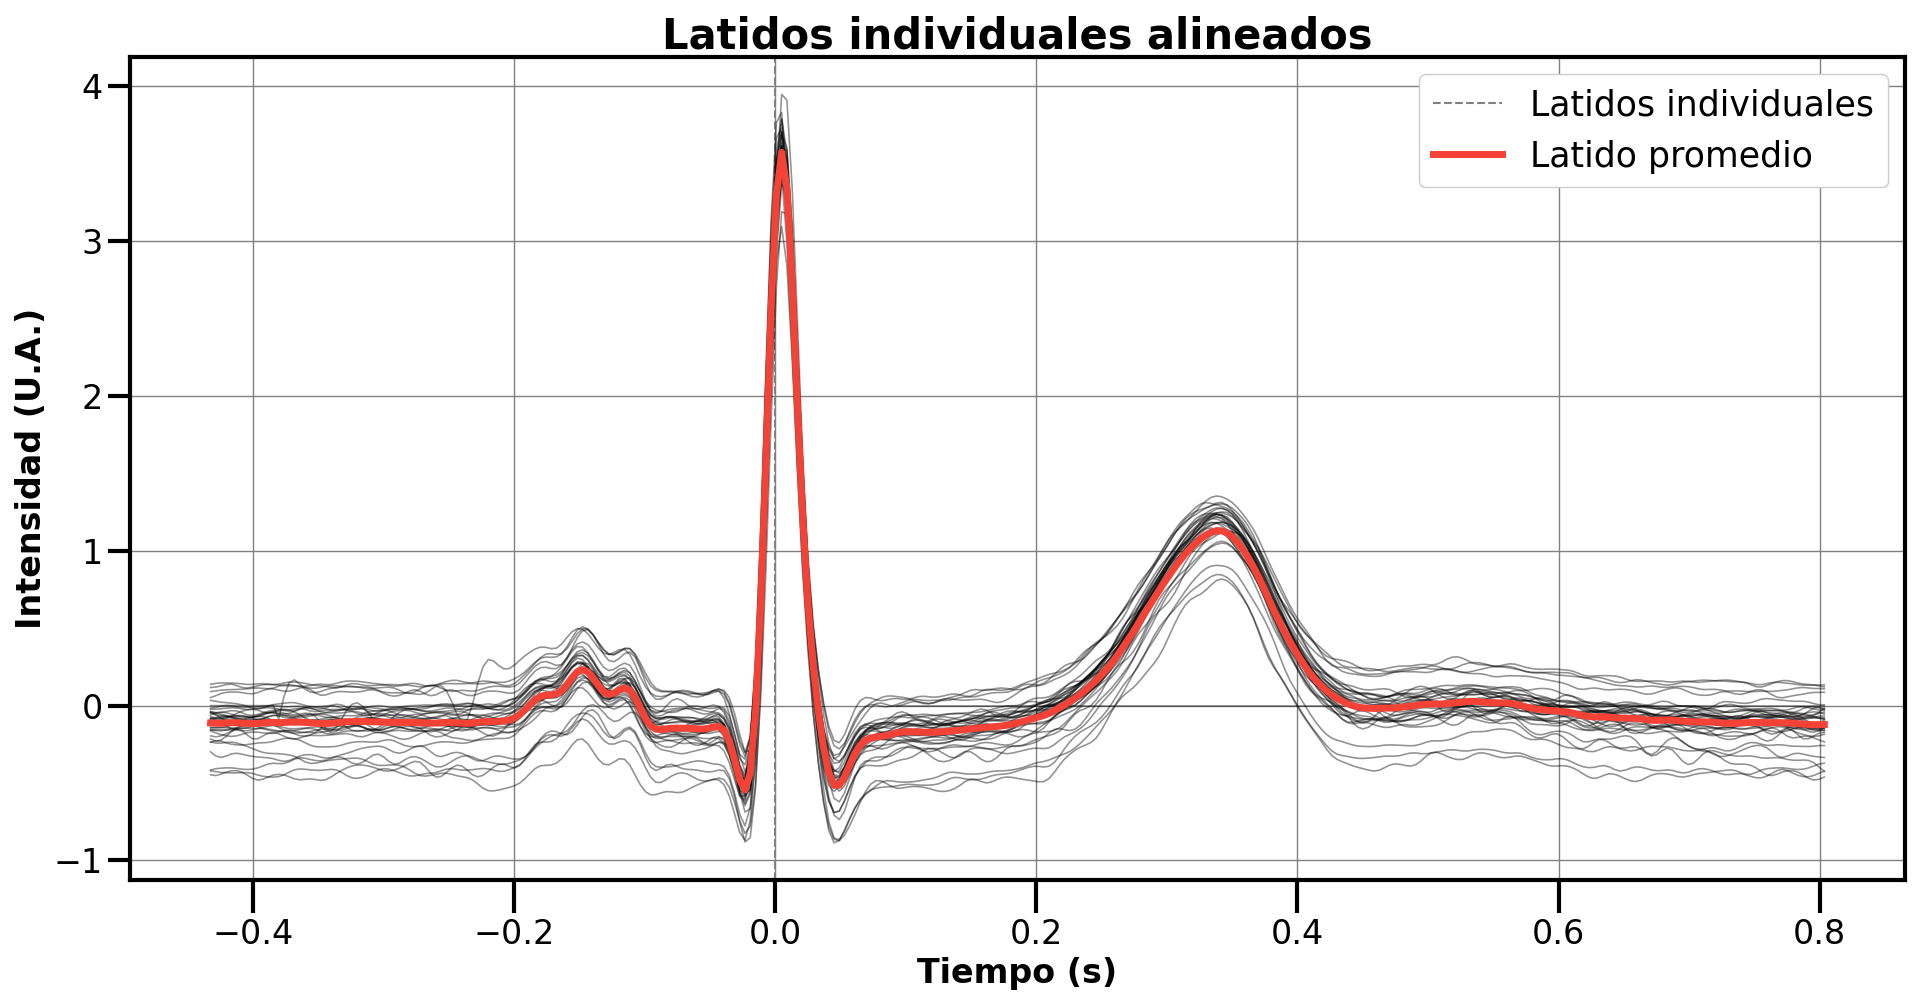
\includegraphics[width=0.85\linewidth]{Sem_1/figuras/ecg_latidos_alineados.png}
	\caption{ECG con latidos individuales alineados.}
	\label{fig:latidos_alineados}
\end{figure}

\subsection{Vector de características} 

Debido a que cada señal ECG ha sido grabada con diferentes modelos de electrocardiógrafos y cada uno de estos posee una frecuencia de muestreo distinta, lo que resulta en latidos promedios con longitudes muéstrales inconsistentes. Para garantizar la comparabilidad morfológica y la viabilidad computacional en etapas posteriores, se implementa una estandarización de longitud fija mediante remuestreo digital. Cada latido se interpola a 250 muestras, este valor preserva la resolución temporal de los eventos cardíacos clave, incluso en ECG de pacientes con trastornos del ritmo cardíaco. Estas señales estandarizadas se almacenan en un arreglo en formato (CSV), este arreglo guarda los valores que al ser graficados, representan la figura del latido promedio de cada paciente, similar a como se observa en la figura \ref{fig:latidos_alineados} (línea roja). 
Este arreglo encapsula de manera compacta la dinámica completa y variaciones inter-paciente en morfología del ciclo cardíaco. Esta representación es fundamental ya que permite que PCA pueda detectar patrones correlacionados entre intervalos, segmentos y demás métricas intrínsecas del latido promedio, además la estructura vectorial numérica es algo que PCA maneja de manera eficiente. Este latido promedio es el denominado vector de características que será la base del análisis de la señal electrocardiográfica. 

\section{Reducción de dimensionalidad}

La reducción de la dimensionalidad es el proceso de encontrar un espacio dimensionalmente reducido adecuado para representar los datos originales, con la esperanza de que la representación alternativa de los datos permita:
\begin{itemize}
	\item Explorar datos de alta dimensión con el objetivo de descubrir una estructura o patrones que conducen a la formación de hipótesis estadísticas.
	\item Visualización de los datos utilizando diagramas de dispersión cuando la dimensionalidad es reducida a 2D o 3D.
	\item Analizar los datos utilizando métodos estadísticos, como la agrupación, suavizado, estimación de densidad de probabilidad o clasificación.
\end{itemize}

Un posible método para la reducción de dimensionalidad seria crear nuevas variables que sean funciones o combinaciones lineales de los segmentos e intervalos que se observan en la figura \ref{fig:ECGSinusal}, pero un método que permite hacer esto internamente, es el conocido como análisis de componentes principales (PCA) \cite{martinez05}. Habiendo culminado la etapa de preprocesamiento de los datos y la extracción de características de los ECG, se procede a la implementación del análisis de componentes principales. Es de destacar que debido al aumento en el uso de las herramientas de aprendizaje automático, la optimización de estas ha magnificado también. Para este trabajo, se utiliza la función \emph{PCA()} de la librería \textbf{scikit-learn (v1.4.2)} \cite{scikit-learn,sklearn_api}, esta función efectúa eficientemente los cálculos subyacentes, como la descomposición de la matriz de covarianza y la solución al posterior problema de autovalores y autovectores. Entre los diversos parámetros que necesita esta función para ser ejecutada, esta el numero final de componentes principales $(k)$, para determinar el numero final de estas se utiliza el criterio de varianza acumulada explicado en la subsección \ref{subsec:PCA}.
El gráfico de la varianza acumulada 

\subsection{Proyección de los vectores de características al nuevo espacio}

Una vez determinadas las componentes principales, se proyectan los vectores de características $I$ al nuevo espacio dimensional reducido $V$ (conjunto de autovectores), esto es: 
\begin{equation}
	P = I \ast V
	\label{eq:proyeccion_pca}
\end{equation}
Este proceso no es una simple comprensión, sino una reestructuración de la información morfológica de cada latido. 
Estos vectores de características, que graficados se ven como la linea roja de la figura \ref{fig:latidos_alineados} se convierten en un vector único para cada latido promedio de cada paciente, con ahora menos dimensiones, como se observa en la tabla \ref{tab:vector_caracteristicas_proyectado}. A El conjunto de todas las proyecciones hechas se le conoce cómo la base de conocimiento de la red neuronal, estás serán usadas en las fases de entrenamiento y prueba de las redes neuronales, esta base de conocimiento se guarda en forma matricial, con las columnas debidamente identificadas con el numero de cada componente y donde cada fila corresponde al latido promedio de un segmento de ECG de cierto paciente, posteriormente dicha base de conocimiento, se guarda en un archivo de formato CSV, que será usado más adelante.
\begin{table}[ht]
	\renewcommand{\arraystretch}{1.2}
	\begin{center}
		\begin{tabular}{|>{\centering} p{2.6cm} | c |}
			\hline
			\textbf{Componente principal} & \textbf{Valor} \\ \hline
			1 & 9.40004 \\ \hline
			2 & -3.47597 \\ \hline
			3 & -1.42403 \\ \hline
			4 & 4.60353 \\ \hline
			5 & -2.69767 \\ \hline
			6 & -0.75595 \\ \hline
		\end{tabular}
	\caption{Ejemplo de vector de características proyectado en el espacio $V$}
	\label{tab:vector_caracteristicas_proyectado}
	\end{center}
\end{table}


\section{Modelado predictivo}

Con el fin de probar que la representación compacta del latido promedio obtenida mediante PCA contiene información suficiente para clasificar e identificar las variables objetivos de las que se nombraron en la subsección \ref{subsec:diseno_investigacion}. Para ello se diseñan algunas redes neuronales, cada una de estas, con una arquitectura que se elige según el tipo de tarea que se desea resolver. Recordemos que el núcleo de esta investigación yace en la búsqueda de agrupaciones en data de señales ECG aprovechando la reducción de dimensionalidad del análisis de componente principales y las habilidades intrínsecas de las redes neuronales perceptrónicas en encontrar correlaciones en la data que se usa como entrada en estas.

\subsection{Algoritmo}

En la subsección \ref{subsec:NN} se explicó detalladamente lo que es una red neuronal, cómo se asemejan estas a una red de tipo biológica, se habló de la unidad básica que se equipara con una neurona y de las dos fases de modelización de una red neuronal. Hoy en día, el diseño a detalle de uno de estos programas se suele hacer sobre interfaces que facilitan la implementación de estos. A estas interfaces se les conoce como frameworks\footnote{Marcos de trabajo.}, uno de los más conocidos y usados es \textbf{TensorFlow} \cite{tensorflow15} este es un ecosistema completo que ayuda a resolver problemas complejos con aprendizaje automático ofreciendo varios niveles de abstracción con el fin de adecuarse a las necesidad del usuario, con la API (interfaz de programación de aplicación, por sus siglas en inglés) de alto nivel de Keras \cite{keras15}, que ayuda a que los primeros pasos con TensorFlow y el aprendizaje automático sean sencillos. 

Si bien TensorFlow permite construir una red neuronal apilando capas como bloques Lego, es decir, este framework proporciona un esquema modular que simplifica el ensamble de las redes neuronales, además, elegir otros hiperparámetros de la red, como las funciones de activación de cada capa, resulta intuitivo. Sin embargo, es crucial enfatizar que los principios matemáticos permanecen idénticos a una implementación manual que se hiciera desde cero, estos son: 
\begin{enumerate}
	\item \textbf{La propagación hacia adelante:} la salida de cada capa $y_l$ sigue siendo la ecuación \ref{eq:percept}, dicha salida será la entrada de la siguiente capa. 
	\item \textbf{Algoritmo de retropropagación:} entre los métodos de optimización de la red en retropropagación existentes, TensorFlow permite seleccionar entre un amplio catalogo, en esta investigación se hizo uso del optimizador \emph{Adam}, que es un método estocástico de descenso de gradiente que se basa en la adaptación de momentos de primer y segundo orden \cite{keras15}. Según Kingma et al. \cite{adamoptimization14} el método es: \begin{quote}
		\textquote{eficiente desde el punto de vista computacional, requiere poca memoria, es invariable frente al cambio de escala diagonal de los gradientes y resulta adecuado para problemas con un gran número de datos/parámetros.}
	\end{quote}
	TensorFlow también permite elegir entre una extensa gama de funciones para el calculo del error entre la salida esperada y la salida de la red en cada iteración, estas funciones se seleccionan en base al uso final de la red que se diseñe, es decir, la función de perdida se elige según la tarea predictiva, por ejemplo, se emplea la entropía cruzada binaria en tareas de clasificación binaria ya que su uso es idóneo cuando las clases son mutuamente excluyentes y la salida usa una única neurona con función de activación tipo sigmoidea. Para clasificaciones multiclase, es recomendable usar la función de perdida denominada entropía cruzada categórica, esta función opera con una capa \emph{softmax} de $M$ neuronas, escalando eficientemente para problemas con decenas o hasta incluso cientos de clases, como identificación de pacientes.
\end{enumerate}

\subsection{Tareas de modelado propuestas} \label{subsec:tareas_modelado}

El diseño de las tareas de modelado en esta investigación se fundamente en el principio de aprovechar las anotaciones clínicas y demográficas disponibles de las bases de datos de Physionet. Estas etiquetas ---asentadas por expertos--- constituyen esas \textquote{verdades base} que permiten que las redes neuronales puedan identificar posibles patrones morfológicos presentes en el latido promedio, y que estos sean variables predictoras con relevancia en futuros pronósticos o clasificaciones. Las tareas que se implementaran son:
\begin{enumerate}
	\item \label{item:clasificacion_salud} \textbf{Clasificación por estado de salud:} si bien la mayoría de las bases de datos nombradas en la \ref{subsec:muestra} albergan el diagnostico clínico de los pacientes presentes, en muchos de los casos, estos no son lo suficientemente detallados como para usar estas anotaciones como \textquote{verdad base}. Por ejemplo, en la base de datos BIDMC de pacientes con insuficiencia cardíaca congestiva severa \cite{InsuficienciaCardiacaDB}, no se detalla el tipo preciso de insuficiencia cardíaca, sólo se sabe que los electrocardiogramas presentes en esta base de datos corresponden a pacientes con insuficiencia cardíaca clase 3 o clase 4. También, en el conjunto de las 48 grabaciones presentes en la base de datos Arritmia \cite{arritmiadb} se conocen que son pacientes con trastornos en el ritmo cardíaco, sin embargo, algunos pacientes tienen presentes distintos tipos de latidos arrítmicos en su señal ECG. Esto hace complicado y extenso el numero de variables objetivo que se le pedirá a la red neuronal que identifique. Es por esto que se eligió sólo clasificar a los pacientes entre \textquote{sanos} y \textquote{patológicos}
	\item \textbf{Predicción por grupos etarios:} uno de los criterios de selección fue que cada registro tenga la edad del paciente al que se le realizó el ECG hacer, este dato se usó como variable objetivo y se encasillaron a todos los pacientes en 3 grupos etarios, los rangos de dichos grupos están tabulados en la tabla \ref{tab:grupos_etarios}.
	\begin{table}[ht]
		\renewcommand{\arraystretch}{1.2}
		\begin{center}
			\begin{tabular}{| M{3cm} | M{2cm} |}
				\hline
				\textbf{Grupos etarios} & \textbf{Rango de edades (años)} \\ \hline
				Jóvenes & 18 - 24 \\ \hline
				Mediana edad & 35 - 59 \\ \hline
				Mayores & 60 - 99 \\ \hline
			\end{tabular}
		\caption{Rangos de los grupos etarios.}
		\label{tab:grupos_etarios}
		\end{center}
	\end{table}
	\item \textbf{Clasificación por sexo:} así como cada registro seleccionado posee la edad del paciente a quien se le realizo el ECG, también debe poseer el sexo biológico de dicha persona, ya que este dato también es una variable objetivo que será usada por la red para clasificar a cada ECG por su sexo.
	\item \textbf{Clasificación por tipo de trastorno de salud:} Debido a lo mencionado en el literal \ref{item:clasificacion_salud} de esta subsección, se decidió por clasificar las cardiopatías similares como correspondientes a un único tipo de trastorno. De acá surgen las categorías que se pueden observar en la tabla \ref{tab:tipos_trastornos}
	\begin{table}[ht]
		\renewcommand{\arraystretch}{1.2}
		\begin{center}
			\begin{tabular}{| M{5cm} | M{8cm} |}
				\hline
				\textbf{Tipos de trastornos} & \textbf{Descripción} \\ \hline
				Trastornos de la respiración durante el sueño & Pacientes con apnea de sueño \\ \hline
				Trastornos del ritmo cardíaco & Pacientes con problemas arrítmicos \\ \hline
				Trastornos de la función de bomba del corazón & Pacientes con insuficiencias cardíacas \\ \hline
				Sanos & Pacientes catalogados como sanos. \\ \hline
			\end{tabular}
		\caption{Tipos de trastornos encontrados.}
		\label{tab:tipos_trastornos}
		\end{center}
	\end{table}
	\item \textbf{Identificación del paciente:} por último, se toma ahora como variable objetivo el nombre de identificación único por paciente (ID), esté será usado para explorar la posibilidad de la existencia de una \textquote{huella digital cardíaca}, ya que si una red neuronal es capaz de identificar a cada paciente usando el latido promedio de este dimensionalmente reducido, podría indicar que existen patrones internos dentro de la morfología del latido, que son únicos entre cada persona.
%	\coffeestainA{0.8}{0.83}{45}{5cm}{1cm}
	
	
\end{enumerate}


\subsection{Preparación de datos}

Para iniciar con el proceso de entrenamiento de las redes neuronales es necesario aplicar un proceso previo a los datos dimensionalmente reducidos que se tienen luego del PCA, recordemos que estos fueron previamente guardados en un archivo CSV donde en cada fila de este, se guardan las componentes principales que estén bajo el umbral de la varianza acumulada fijado, además este archivo contiene el ID de cada paciente. Como datos de entrada en todas las redes se usaron las primeras 20 componentes principales de cada latido, además se dividió la data en un 60\% para entrenamiento y un 40\% para posteriores pruebas o validaciones. 

\subsection{Arquitecturas empleadas (casos con PCA)}
\label{subsec:arquitecturas_pca}
Debido a la naturaleza diferente de cada tarea que se propone en la subsección \ref{subsec:tareas_modelado}, es necesario diseñar redes neuronales con arquitecturas que se ajusten a los requerimientos de cada tarea de modelado, es por esto que se plantean los siguientes modelos de redes neuronales:

\begin{enumerate}
	\item \textbf{Clasificación por estado de salud:} recordemos que esta tarea es un problema de clasificación binaria (\textquote{sano} vs. \textquote{patológico}), por ende, se propone una red neuronal de capas densas con topología (10-1), como se observa en la tabla \ref{tab:summary NN estado de salud}. Estas neuronas emplean como función de activación en las capas ocultas la función ReLU y la función Sigmoide en la capa de salida, optimizada mediante el algoritmo Adam \cite{adamoptimization14}, para esta red se seleccionó la denominada entropía cruzada categórica, como función de perdida. 
	
	\begin{table}[ht]
		\renewcommand{\arraystretch}{1.2}
		\begin{center}
			\begin{tabular}{| M{2.5cm} | M{3cm} | M{3cm} |}
				\hline
				\textbf{Capa (tipo)} & \textbf{Número de neuronas} & \textbf{Función activación} \\ \hline
				Densa & 10 & ReLU    \\ \hline
				Densa & 1 & Sigmoide \\ 
				\hline
			\end{tabular}
		\end{center}
		\caption{Arquitectura de la red neuronal para la clasificación por estado de salud.}
		\label{tab:summary NN estado de salud}
	\end{table}
	\item \textbf{Predicción por grupos etarios:} el modelo multiclase para grupos etarios utiliza una arquitectura de 4 capas con (10-15-10-3) neuronas por cada capa; y funciones de activación ReLU y Sigmoide para las capas ocultas y la capa de salida respectivamente, como se observa en la tabla \ref{tab:summary NN grupos etarios}, en este caso la red fue entrenada usando la función de perdida denominada entropía cruzada binaria. 
	\begin{table}[ht]
		\renewcommand{\arraystretch}{1.2}
		\begin{center}
			\begin{tabular}{| M{2.5cm} | M{3cm} | M{3cm} |}
				\hline
				\textbf{Capa (tipo)} & \textbf{Número de neuronas} & \textbf{Función activación} \\ \hline
				Densa & 10 & ReLU    \\ \hline
				Densa & 15 & ReLU    \\ \hline
				Densa & 10 & ReLU    \\ \hline
				Densa & 3 & Sigmoide \\
				\hline
			\end{tabular}
		\end{center}
		\caption{Arquitectura de la red neuronal para la predicción por grupos etarios.}
		\label{tab:summary NN grupos etarios}
	\end{table}
	\item \textbf{Clasificación por sexo:} la red binaria para clasificación por sexo emplea una arquitectura menos liviana que las anteriores (20-20-20-20-1) con función de activación ReLU en capas ocultas y Sigmoide en la capa de salida como se aprecia en la tabla \ref{tab:summary NN clasificacion por sexo}.
	\begin{table}[ht]
		\renewcommand{\arraystretch}{1.2}
		\begin{center}
			\begin{tabular}{| M{2.5cm} | M{3cm} | M{3cm} |}
				\hline
				\textbf{Capa (tipo)} & \textbf{Número de neuronas} & \textbf{Función activación} \\ \hline
				Densa & 20 & ReLU    \\ \hline
				Densa & 20 & ReLU    \\ \hline
				Densa & 20 & ReLU    \\ \hline
				Densa & 20 & ReLU    \\ \hline
				Densa & 1 & Sigmoide \\
				\hline
			\end{tabular}
		\end{center}
		\caption{Arquitectura de la red neuronal para la clasificación por sexo.}
		\label{tab:summary NN clasificacion por sexo}
	\end{table}
	
	\item \textbf{Clasificación por tipo de trastorno de salud:} Para el modelo de clasificación multiclase por estados de salud, se diseñó una red neuronal con 3 capas densas y una capa de salida con 4 neuronas correspondientes a las 4 categorías de tipos de trastornos mencionados en la tabla \ref{tab:tipos_trastornos}, la cantidad de neuronas por capa y su función de activación se detallan en la tabla \ref{tab:summary NN clasificacion por trastorno}
	\begin{table}
		\renewcommand{\arraystretch}{1.2}
		\begin{center}
			\begin{tabular}{| M{2.5cm} | M{3cm} | M{3cm} |}
				\hline
				\textbf{Capa (tipo)} & \textbf{Número de neuronas} & \textbf{Función activación} \\ \hline
				Densa & 10 & ReLU    \\ \hline
				Densa & 15 & ReLU    \\ \hline
				Densa & 15 & ReLU    \\ \hline
				Densa & 4 & Sigmoide \\ 
				\hline
			\end{tabular}
		\end{center}
		\caption{Arquitectura de la red neuronal para la clasificación por trastorno de salud.}
		\label{tab:summary NN clasificacion por trastorno}
	\end{table}
	
	\item \textbf{Identificación por paciente:} Para la identificación de individuos (761 pacientes), se diseñó una red con 5 capas densas con función de activación ReLU, seguidas de la capa de salida con 10 neuronas, donde, haciendo uso de la función de activación \guillemetleft Hard\_sigmoide\guillemetright \ se observaron los mejores resultados, nótese que la salida equivale a la longitud del identificador binario asignado a cada paciente. En la tabla \ref{tab:summary NN identificacion por paciente} se detalla el estructura de la red.
%	¿Es necesario nombrar todos los Parametros de ajustes de la red
	\begin{table}[ht]
		\renewcommand{\arraystretch}{1.2}
		\begin{center}
			\begin{tabular}{| M{2.5cm} | M{3cm} | M{3cm} |}
				\hline
				\textbf{Capa (tipo)} & \textbf{Número de neuronas} & \textbf{Función activación} \\ \hline
				Densa & 40 & ReLU \\ \hline
				Densa & 35 & ReLU \\ \hline
				Densa & 25 & ReLU \\ \hline
				Densa & 25 & ReLU \\ \hline
				Densa & 15 & ReLU \\ \hline
				Densa & 10 & Hard\_sigmoide \\
				\hline
			\end{tabular}
		\end{center}
		\caption{Arquitectura de la red neuronal para la identificación por paciente.}
		\label{tab:summary NN identificacion por paciente}
	\end{table}
\end{enumerate}


\subsection{Entrenamiento} 

En esta etapa se busca ajustar los pesos sinápticos de la red para minimizar el error que existe entre las salidas predichas y las deseadas, ya que esto es lo que permite que cada red, que ha sido previamente diseñada, aprenda los patrones relevantes de las señales electrocardiográficas dimensionalmente reducidas. Entrenar una red neuronal es un trabajo complejo, matemáticamente hablando, ya que los pesos de cada capa están conectados entre sí y son dependientes unos de otros, es por esto que la modificación de un sólo peso de la capa de entrada repercutirá no sólo en la neurona directamente conectada, sino que se propagará a todas las capas siguientes y por consiguiente a la capa final de la red. Existen bibliotecas computacionales dedicadas al aprendizaje automático, y más específicamente a redes neuronales, estas tienen implementadas funciones y métodos que automatizan el entrenamiento, pero resulta importante conocer dichos procesos para entender cómo las redes adquieren este aprendizaje pudiendo reconfigurar ciertos parámetros para mejorar este aprendizaje. En el área de las redes neuronales hablar de funciones de pérdida o de costo se suele usar como sinónimo y existe una amplia variedad de estas, se selecciona la apropiada para la red neuronal de acuerdo al tipo de problema que se desea solucionar, por ejemplo, para los problemas de clasificación binaria como la clasificación por estado de salud o sexo, se hace uso de la entropía cruzada binaria que no es más que un caso particular de la entropía cruzada categórica utilizada para problemas multiclase, esta función de perdida antes mencionada fue seleccionada para las redes de identificación de grupos etarios y para la red de clasificación por tipo de trastorno de salud. Es importante mencionar que para la red de identificación por paciente, se utilizó el error cuadrático medio como función de perdida. En estos modelos se usó una estrategia de aprendizaje supervisado, dada las características previas de las etiquetas (grupos etarios, tipo de trastorno, sexo e ID de cada paciente) asociadas a los distintos problemas de identificación, se implementó el algoritmo de retropropagación de error, utilizando optimizadores adaptativos como \textit{Adam} y \textit{RMSprop}. La selección de estos optimizadores en cada caso se realizó mediante una evaluación comparativa de su desempeño, optándose por aquel que exhibió las mejores métricas de convergencia en el entrenamiento para la tarea específica bajo consideración. Una vez que los modelos han sido entrenados y se ha obtenido el mejor desempeño, midiéndose este usando la \textit{precisión} (Accuracy, como se conoce en inglés) que no es más que la proporción de todas las clasificaciones que fueron correctas y que se define matemáticamente como se observa en la ecuación \ref{eq:precision}. Una vez se encuentran los parámetros de la red que maximizan la precisión, estos se guardan para la fase de Test.
\begin{equation}
	\label{eq:precision}
	Precision = \frac{Clasificaciones \ correctas}{Clasificaciones \ totales}
\end{equation}

\subsection{Test}

En esta fase, se procede a validar el funcionamiento de la red neuronal utilizando los parámetros optimizados y guardados durante la fase previa de entrenamiento. Para ello, se utilizan los datos reservados para validación, que corresponden a un 40\% del total del conjunto de datos original, garantizando así que el modelo sea evaluado con información que no ha sido vista durante el aprendizaje. Estos datos de validación se ingresan como entradas a la red, y las salidas predichas se comparan con las salidas reales conocidas para calcular métricas de desempeño, siendo la precisión como la principal medida cuantitativa empleada. Además, se utiliza una matriz de confusión para visualizar de manera detallada cómo se distribuyen las predicciones correctas e incorrectas entre las diferentes clases o categorías. Esta matriz permite identificar el número de verdaderos positivos, verdaderos negativos, falsos positivos y falsos negativos, lo que facilita la interpretación del rendimiento del modelo en cada clase específica. De esta forma, se logra cuantificar el nivel de exactitud del modelo entrenado.

\section{Reducción no lineal de dimensionalidad (t-SNE)}

A partir de los resultados obtenidos mediante el análisis de componentes principales (PCA), se procedió a realizar un análisis exploratorio adicional aplicando t-SNE, una técnica avanzada de reducción no lineal de dimensionalidad y visualización de agrupaciones en datos de alta dimensiones. Con este proceso, se busca principalmente evaluar la representación de las diferentes señales electrocardiográficas en un espacio de menor dimensión que facilite la identificación de patrones y posibles estructuras de agrupamiento, preservando las relaciones de similitud entre estas señales. Para ellos, se seleccionaron y ajustaron los hiperparámetros más adecuados del algoritmo t-SNE ---como la perplejidad y el número de iteraciones máximo--- en base a la experimentación y el análisis visual de los resultados, buscando configuraciones que optimicen la claridad de los agrupamientos en la proyección final.

Seleccionar la configuración optima de t-SNE no es directa como en el caso de PCA, donde nos valemos de algún método de validación interna para determinar el número apropiado de componentes principales, con t-SNE es necesario realizar múltiples ejecuciones del algoritmo variando los hiperparámetros clave, mencionados anteriormente, para esto, se configura el número de componentes de salida a $2$, esto con el fin de agilizar el proceso y así poder facilitar la visualización bidimensional de los datos. El análisis visual de los resultados permitió evaluar la capacidad de separación de los grupos obtenidos bajo diferentes combinaciones de parámetros, identificando aquellos que maximicen la conservación de las estructuras de interés. Una vez se hayan definido los parámetros óptimos, se procede a ejecutar el algoritmo antes mencionado nuevamente, empleando las configuraciones definidas previamente, pero esta vez solicitando $3$ componentes como salida, conservando así una representación tridimensional resultante para su uso posterior en los análisis y modelos desarrollados.

\subsection{Arquitecturas de redes neuronales para interpretación de t-SNE}

Si bien t-SNE es una herramienta poderosa para la reducción de dimensionalidad y la visualización de datos complejos, su interpretación directa plantea dificultades debido a su naturaleza no lineal, la sensibilidad a los hiperparámetros y el hecho de que la estructura global puede distorsionarse o perder significado clínico relevante. Por esta razón, para traducir las representaciones obtenidas mediante t-SNE a variables clínicas conocidas y facilitar su interpretación desde una perspectiva biomédica, se hace necesario emplear modelos adicionales. En este caso, se diseñaron arquitecturas de redes neuronales específicamente orientadas a funcionar como traductores entre los componentes generados por t-SNE y las variables clínicas de interés, permitiendo así analizar y aprovechar los patrones extraídos en el espacio reducido para tareas de identificación o clasificación antes mencionadas. Todas las redes neuronales desarrolladas para traducir las representaciones generadas por t-SNE comparten una arquitectura homogénea, compuesta por el mismo número de capas y la misma cantidad de neuronas en cada una de ellas. La única diferencia radica en la configuración de la capa de salida, la cual se adapta específicamente a la naturaleza de la variable clínica que se busca predecir en cada caso, permitiendo así ajustar el modelo a las particularidades de cada problema. En la tabla 
\ref{tab:summary NN comun a tsne} se detalla la estructura de las capas internas de las redes propuestas.

\begin{table}[ht]
	\renewcommand{\arraystretch}{1.2}
	\begin{center}
		\begin{tabular}{| M{2.5cm} | M{3cm} | M{3cm} |}
			\hline
			\textbf{Capa (tipo)} & \textbf{Número de neuronas} & \textbf{Función activación} \\ \hline
			Densa & 20 & ReLU    \\ \hline
			Densa & 20 & ReLU    \\ \hline
			Densa & 20 & ReLU    \\ \hline
			Densa & 20 & ReLU    \\ \hline
			Densa & 20 & ReLU    \\ \hline
			Densa & 20 & ReLU    \\ \hline
			Densa & 20 & ReLU    \\ \hline
			Densa & 20 & ReLU    \\ 
			\hline
		\end{tabular}
	\end{center}
	\caption{Arquitectura común de las redes neuronales propuestas para la interpretación de los datos t-SNE.}
	\label{tab:summary NN comun a tsne}
\end{table}

En la tabla \ref{tab:summary NN salidas problemas tsne} se contemplan las características de las capas de salida para cada modelo propuesto.% es de resaltar que no se desarrolló una red neuronal que pueda traducir los datos pos t-SNE

\begin{table}[ht]
	\renewcommand{\arraystretch}{1.2}
	\begin{center}
		\begin{tabular}{| M{2.5cm} | M{3cm} | M{3cm} |}
			\hline
			\textbf{Tipo de clasificación} & \textbf{Número de neuronas} & \textbf{Función de activación} \\ \hline
			Estado de salud   & 1 & Sigmoide \\ \hline
			Grupos etarios    & 3 & Sigmoide \\ \hline
			Sexo              & 1 & Sigmoide \\ \hline
			Tipo de trastorno & 4 & Sigmoide \\ 
			\hline
		\end{tabular}
	\end{center}
	\caption{Características de las capas de salida para cada red propuesta según el tipo de clasificación}
	\label{tab:summary NN salidas problemas tsne}
\end{table}

%No se hizo una red neuronal para identificar a los pacientes, debido a la baja accuracy que se logró usando tsne
%\subsection{K-means}



\section{Validez y confiabilidad}

\subsection{Validación de modelos}

Con el fin de validar los resultados salientes de las redes neuronales de manera objetiva y sistemática, durante el proceso de entrenamiento de las redes neuronales, se dividió el conjunto de datos para entrenamiento y validación, en 60\% y 40\% para cada subconjunto respectivamente, lo que asegura que la evaluación de desempeño se realice sobre instancias no vistas durante la fase de entrenamiento. En este proceso, se emplean los parámetros óptimos obtenidos en el entrenamiento y se calculan métricas como la precisión, lo que permite determinar la capacidad de generalización de los modelos propuestos. Para dar mayor detalle a la distribución de las predicciones correctas e incorrectas por clase, se construyen matrices de confusión. Este marco de trabajo asegura que el rendimiento reportado sea representativo y confiable, lo que suporta la robustez de la solución planteada.

\subsection{Clasificación}

Para las tareas de clasificación, las redes neuronales fueron evaluadas en su capacidad para distinguir entre diferentes categorías, como estado de salud, sexo, grupo etario y tipo de trastorno cardíaco. La robustez del procedimiento se garantiza al emplear etiquetas clínicas definidas por expertos, permitiendo que los resultados de clasificación sean tanto cuantitativos como clínicamente relevantes. Las arquitecturas de las redes neuronales, funciones de activación y optimizadores, fueron adaptados en función del problema específico, logrando un balance adecuado entre interpretabilidad y rendimiento. 

\subsection{Dendrograma}

Un dendrograma es un diagrama que muestra la relación jerárquica entre objetos. Por lo general, se crea como resultado de un agrupamiento jerárquico. El uso principal de un dendrograma es encontrar la mejor manera de asignar objetos a grupos. El dendrograma siguiente, figura \ref{fig:dispersion_dendrograma} muestra la agrupación jerárquica de seis observaciones que se muestran en el diagrama de dispersión de la izquierda \cite{whatsdendro}

\begin{figure}[h]
	\centering
	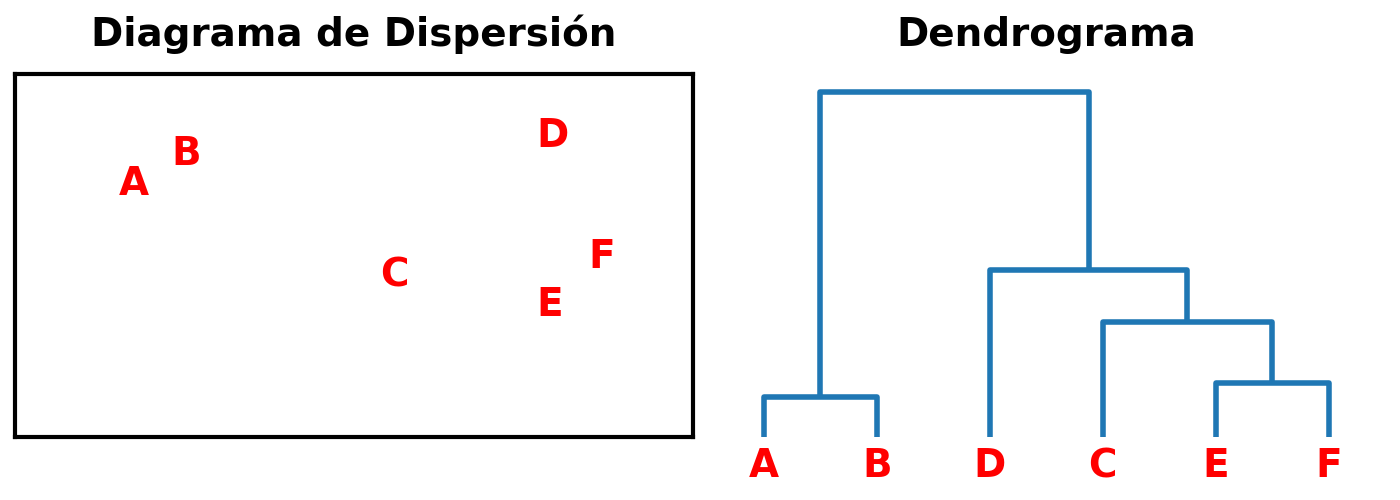
\includegraphics[width=0.85\linewidth]{Sem_1/figuras/Dispersion_diagrama_1.png}
	\caption{Diagrama de dispersión y su dendrograma.}
	\label{fig:dispersion_dendrograma}
\end{figure}

La clave para interpretar un dendrograma es centrarse en la altura a la que se unen dos objetos. En el ejemplo anterior, podemos ver que E y F son más similares, ya que la altura del enlace que los une es la más pequeña. Los siguientes dos objetos son más similares son A y B. 

En el dendrograma anterior, la altura indica el orden en el que se unieron los grupos. Se puede crear un dendrograma más informativo donde las alturas reflejan la distancia entre los grupos, como se muestra en la figura \ref{fig:dispersion_dendrograma}. En este caso, el dendrograma muestra que la gran diferencia entre los conglomerados está entre el conglomerado de A y B versus el de C, D, E y F.

Es importante apreciar que el dendrograma es un resumen de la matriz de distancias y, como ocurre con la mayoría de los resúmenes, se pierde información. Por ejemplo, el dendrograma sugiere que C y D están mucho más cerca entre sí que C a B, pero los datos originales (que se muestran en el diagrama de dispersión) muestran que esto no es cierto. La consecuencia de la pérdida de información es que los dendrogramas son más precisos en la parte inferior, mostrando qué elementos son muy similares \cite{whatsdendro}

\subsubsection{Asignar observaciones a conglomerados}

Las observaciones se asignan a los conglomerados trazando una línea horizontal a través del dendrograma. Las observaciones que se unen por debajo de la línea están agrupadas. En la figura \ref{fig:dispersion_dendrograma_2}
se tienen dos grupos. Un grupo combina A y B, y un segundo grupo combina C, D, E y F.
\begin{figure}[H]
	\centering
	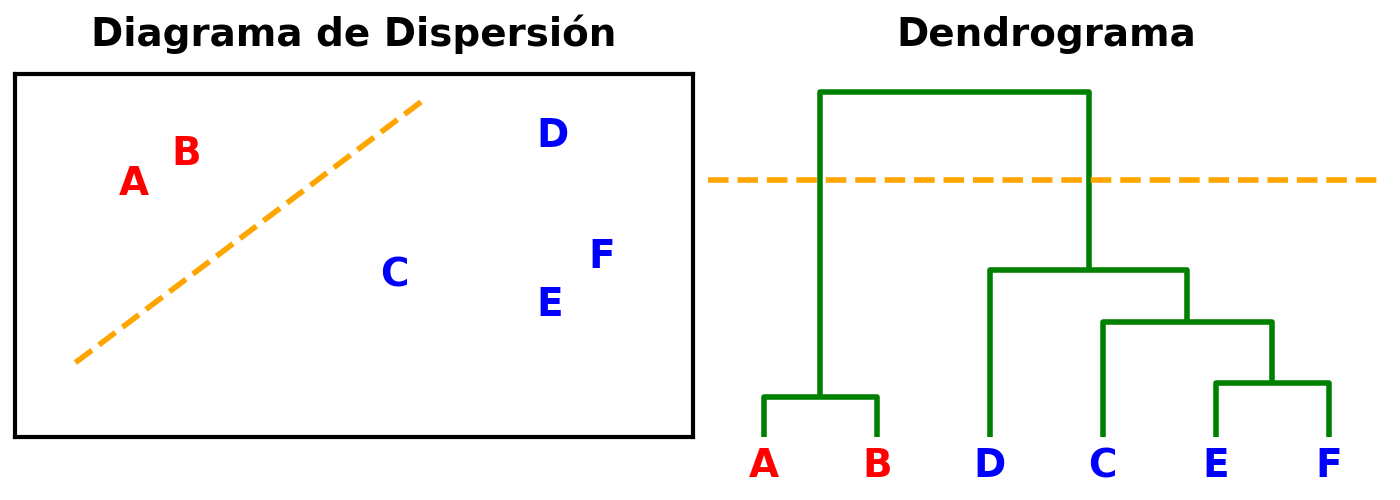
\includegraphics[width=0.85\linewidth]{Sem_1/figuras/Dispersion_diagrama_2.png}
	\caption{Asignación de observaciones a conglomerados.}
	\label{fig:dispersion_dendrograma_2}
\end{figure}

Un error común que se comete al leer dendrogramas es asumir que la forma del dendrograma da una pista de cuántos grupos existen. En el ejemplo anterior, la interpretación (incorrecta) es que el dendrograma muestra que hay dos grupos, ya que la distancia entre los grupos (los segmentos verticales del dendrograma) es mayor entre dos y tres grupos. Los dendrogramas a menudo sugieren un número correcto de agrupaciones cuando no hay evidencia real que apoye la conclusión \cite{whatsdendro}.

\subsection{Repetibilidad}

Para garantizar la repetibilidad de los resultados, se realizaron múltiples ejecuciones independientes de los modelos, variando únicamente la semilla aleatoria %usada por las redes neuronales para inicializar los pesos sinapticos 
y manteniendo constantes las condiciones de entrenamiento y validación. Este enfoque permite certificar que los modelos ofrecen resultados fiables independientemente de las condiciones iniciales, y que los patrones, que son identificados por las redes neuronales, son reproducibles y no producto del azar. 


\subsection{Consideraciones éticas}

El proceso metodológico implementado en esta investigación considera de forma estricta los principios éticos asociados al manejo de datos biomédicos. Los registros de ECG utilizados fueron anonimizados para preservar la confidencialidad de la información clínica de los participantes, cumpliendo con las normativas internacionales de protección de datos. 
% Se enfatiza que la interpretacion y uso de los modelos automaticos debe estar siempre supervisada por expertos clinicos, reconociendo que las decisiones medicas requieres una evaluacion integral que los algoritmos no pueden sustituir, sino complementar de manera responsable.
%Poner eso en las recomendaciones


\chapter{Resultados}

\section{Descripción general de los datos}

Cabe destacar que las señales electrocardiográficas que se tienen provienen de la segmentación de las señales originales tomadas de la cantidad total de pacientes reflejados en la tabla \ref{tab:distriECGs}, es por esto que se observará en las siguientes tablas, un aumento significativo de estas señales.

Inicialmente se tiene un total de 8540 señales electrocardiográficas, en edades comprendidas entre 18 y 90 años, se establecen tres grupos etarios para poder estudiar para poder estudiar el comportamiento

\begin{table}
	\renewcommand{\arraystretch}{1.2}
	\begin{center}
		\begin{tabular}{| M{2cm} | M{2cm} | M{0.8cm} | M{0.8cm} | M{0.8cm} | M{2cm} | M{2.2cm} |}
			\hline
			\textbf{Grupo etarios (años)} & \textbf{Cantidad} & \textbf{\%} & \textbf{M} & \textbf{F} & \textbf{Edad promedio} & \textbf{Desviación} \\ \hline 
			(18-34)	& 5131 & 60   & 1970 & 3161 & 24.2  & 4.0  \\ \hline
			(35-59)	& 1476 & 17.3 & 752  & 724  & 45.50 & 6.7  \\ \hline
			(> 60)	& 1933 & 22.7 & 694  & 1239 & 73.84 & 7.7  \\ \hline
	\textbf{Total}	& 8540 &      & 3416 & 5124 &		&	   \\ \hline
		\end{tabular}
	\end{center}
	\label{}
	\caption{}
\end{table}



\subsection{Distribuciones de los sujetos sanos por sexo y grupos etarios}

\subsection{Distribuciones de los sujetos patológicos por sexo y grupos etarios}

\section{Descripción general de PCA}

\subsection{Método de la varianza acumulada}
Pequeña discusión

\subsection{Gráficas de pca de los datos, 2 componentes, probando varias combinaciones}
Y su respectivo análisis o discusión

\section{Resultados de clasificación usando los datos de PCA}
¿se ponen los gráficos de entrenamiento de las redes?

\subsection{Metricas de desempeño}
¿Correr varias veces para calcular a posteriori alguna estadística?


\subsection{Matrices de confusión}
análisis de este

\section{Resultados de identificacion de pacientes}

\subsection{metricas de desempeño}

\subsection{Matrices de confusión}

\subsection{Discusion sobre la viabilidad de la huella digital cardíaca}


\section{Analisis exploratorio tsne}
¿Se puede mostrar quizas algunas graficas en 2d de tsne donde se vean los pequeños agrupamientos?

\section{Resultados de clasificacion usando los datos de tsne}

\subsection{Metricas de desempeño}

\subsection{Matrices de confusion}
análisis de estas

\subsection{Dendrogramas}



%\part{Conclusiones}
\chapter{Conclusiones}

...

% Bibliografía
\bibliographystyle{ieeetr}
\bibliography{bibliografia.bib} 

\end{document}
